\documentclass[12pt,french]{book}
\usepackage[utf8]{inputenc}
\usepackage{fancyhdr}
\usepackage[frenchb]{babel}
\usepackage[french]{minitoc}
\usepackage{microtype}
\usepackage{lipsum}
\usepackage{caption}
\usepackage{tikz}
\usetikzlibrary{arrows}
\usetikzlibrary{positioning}
\usepackage[nottoc, notlot]{tocbibind} 
\usepackage{geometry}
\usepackage{graphicx}
\usepackage{subfig}
\usepackage{booktabs}
\geometry{hmargin=2.5cm,vmargin=2.5cm}
\usepackage{epic,eepic,amssymb,amsmath,amsfonts}
%\usepackage{times}
%\usepackage{hyperref}% référence vers equation
\usepackage{setspace}
\linespread{1.5}
% biblio ordonnee classique
\bibliographystyle{unsrt} 
\pagestyle{fancy}
\renewcommand{\headrulewidth}{1pt}
%\fancyhead[C]{\textbf{page \thepage}} 
\fancyhead[L]{\leftmark}
\fancyhead[R]{ }
% biblio ordonnee classique
\bibliographystyle{unsrt}
\title{Contribution à la modélisation des réseaux complexes}
\author{A. Lachgar, A. Achahbar}
\date{\today}
\begin{document}
%	\sffamily
	%\ttfamily
	%\bfseries
\frontmatter  
% le titre
\maketitle

\chapter*{Remerciements}
% pour faire apparaitre l'introduction dans le sommaire et que les minitocs soient au bon
% endroit
%\addstarredchapter{Introduction générale}  
% Pour que l'entete soit correcte car chapter* ne redefinit pas l'entete.
%\markboth{INTRODUCTION}{}
\addstarredchapter{Remerciements} 
ggggggggggggggggg
 
%
% contenu du fichier : intro.tex
%
\chapter*{Abstract}
% pour faire apparaitre l'introduction dans le sommaire et que les minitocs soient au bon
% endroit
%\addstarredchapter{Introduction générale}  
% Pour que l'entete soit correcte car chapter* ne redefinit pas l'entete.
%\markboth{INTRODUCTION}{}
\addstarredchapter{Abstract} 
Complex networks is a fundamental field of research that model and study artificial and natural networks in our real world. The discovery of common universal properties, almost to all real networks, such as small-world property and scale-free distribution, has revolutionized the way as these networks are studied, modeled and processed.
 A complex network consists of a large number of interacting entities, hence the emergence of properties at large-scale. The object of this thesis is to introduce some contributions to this domaine. In the beginning, we present the state of the art necessary to the readers, next we analyze the model of Barabási and Albert relying on a new model having the complement of the probability of the first one. After, we study uncorrelated scale-free networks, based on simple steps and assumptions. Then, we treat Newman and Watts' small-world model by relying on renormalization group transformation. 
 Finally, we propose a method to predict the type of phase transitions in the percolation phenomenon in the vicinity of the critical point.
%
% contenu du fichier : intro.tex
%
\chapter*{Résumé}
% pour faire apparaitre l'introduction dans le sommaire et que les minitocs soient au bon
% endroit
%\addstarredchapter{Introduction générale}  
% Pour que l'entete soit correcte car chapter* ne redefinit pas l'entete.
%\markboth{INTRODUCTION}{}
\addstarredchapter{Résumé} 
 La science du réseau complexe est un domaine de recherche fondamental pour modéliser les réseaux artificiels et naturels dans notre monde réel. La découverte
 des propriétés universelles communs, presque entre tous les réseaux réels, tel que la propriété petit-monde et la distribution libre-échelle, a révolutionné la façon
 d’étudier, de modéliser et de traiter ces réseaux.
 Un réseau complexe est un réseau d’interactions entre entités d’où l’émergence
 des propriétés à grande échelle.\\ L'objectif de cette thèse est de donner quelques contributions au domaine, en première lieu, nous présentons l’état de l’art nécessaire aux lecteurs, puis nous analysons le modèle de Barabási et Albert en s'appuyant sur un nouveau modèle ayant le complément de la probabilité du premier modèle. Aussi nous étudions les réseaux libre-échelle non corrélés, en basant sur  des étapes et des hypothèses simples, nous obtenons les expressions explicites du nombre des nœuds à une distance donnée d'un nœud arbitraire, profitant de la forme de l'expression obtenu, nous déduirons l'expression explicite de plus court chemin. Après nous traitons le modèle petit-monde de Newman et Watts en basant sur la transformation de groupe de renormalisation, nous commençons par établir une formule plus précise de la fonction universelle déjà trouvé par Newman, Moore et Watts, puis nous montrons que celle-ci n'est pas toujours vrai, cependant il y a une saturation de raccourcis et une nouvelle fonction universelle qui sont apparaît, ainsi que le variable de cette nouvelle fonction est différents de l'ancien, nous en déduisons que l'émergence de la propriété petit-monde dans ce modèle est spectaculaire. En fin nous proposons une méthode afin de prédire le type des transitions de phases au voisinage de point critique, cette méthode s'appuyant sur deux paramètres, le premier est l'exposant de la distribution d'amas au voisinage de point critique, le deuxième est l'exposant de la distribution d'amas avec lesquels les amas se choisissant, nous obtenons que, au voisinage de point critique le type de transition de phase dépend seulement au premier paramètre. 
% table des matieres generale
\tableofcontents
%insere la liste des tableaux
\listoffigures
% inclusion des chapitres
\mainmatter
%
% contenu du fichier : intro.tex
%
\chapter*{Introduction}
% pour faire apparaitre l'introduction dans le sommaire et que les minitocs soient au bon
% endroit
\addstarredchapter{Introduction}  
% Pour que l'entete soit correcte car chapter* ne redefinit pas l'entete.
\markboth{INTRODUCTION}{}
Un réseau complexe est un grand nombre des nœuds liés entre eux selon des topologies de connexion spécifiques. Les réseaux complexes sont omniprésents dans le monde naturel et artificiel grâce aux développements technologiques des $60$ dernières années. En effet,  la plupart des réseaux réels peuvent être représentés par des réseaux complexes, on peut distinguer plusieurs types de réseaux dans les différents domaines, tels que le domaine social, technologique, biologique, physique, etc. Par exemple, un système qui se compose de différents types de molécules qui s'affectent les unes aux autres par des réactions enzymatiques \cite{Je-al2000}, Internet  relie un grand nombre de serveurs et d'ordinateurs dans le monde entier échangeant constamment des quantités gigantesques de paquets d'informations \cite{F-al1999}, le World Wide Web est un réseau virtuel de sites Web liés avec des hyperliens \cite{BA1999}, et les réseaux alimentaires relient également, via des relations trophiques, un grand nombre d'espèces interdépendantes \cite{Co-al1990,Pim-al2002}. Bien que l'existence de ces réseaux dans divers domaines était connue depuis longtemps, les physiciens n'ont commencé à s'y intéresser que depuis la découverte de certaines lois universelles communes à différents systèmes réels. Parmi ces lois les plus importantes on cite: 
\textsf{la distribution de degrés} libre-échelle \footnote{ Libre-échelle signifie qu'il n'y a pas une valeur de degré caractéristique dans le réseau, mais plutôt une distribution de degrés qui suit une loi de puissance.},
%qui rapportée pour la première fois par des mesures d'Internet par Faloutsos et al. []
la propriété \textsf{petit-monde}  
et la valeur élevée du \textsf{coefficient de regroupement} (Clustering). Afin de bien comprendre les comportements de ces réseaux et établir les lois qui les gouvernent, les physiciens, les mathématiciens et les informaticiens se consacrent à développer des modèles théoriques et des techniques permettant de découvrir  et d'analyser les propriétés de ces réseaux qui sont presque partout. Il semble que le début du troisième millénaire va connaître une nouvelle révolution emportée par les principes des réseaux complexes.\\

Il est évident que la physique statistique est l'outil adéquat pour étudier les systèmes ayant un grand nombre d'éléments en interaction. En effet, elle a développé au cours du temps un ensemble de théories et d'outils mathématiques permettant, à partir des comportements microscopiques, de comprendre l'émergence des caractéristiques macroscopiques et d’étudier systématiquement la topologie de ces grands réseaux complexes. En outre la physique statistique est le cadre théorique le plus perfectionné pour étudier les problèmes de transitions de phases et les points critiques, ce qui est incontournable dans l'étude des systèmes complexes. \\

Ce travail de recherche entreprend quelques contributions à la modélisation des réseaux complexes, en abordant quelques problèmes concernant la dynamique de la croissance dans le modèle de Barabási-Albert (BA) \cite{BA1999}, la structure des réseaux  libre-échelle, l'émergence de la propriété petit-monde dans le modèle de Newman-Watts \cite{Newman-Watts1999-2}, et la caractérisation des transitions de phases dans le phénomène de  percolation.
De façon plus détaillée, cette thèse est constituée de cinq chapitres. Le premier commence par définir et mettre en évidence l'importance de notre cadre de recherche (réseaux complexes), et se termine par un état de l'art de  certaines techniques et concepts fondamentaux pertinents de la physique statistique et de la théorie des graphes. Le deuxième chapitre commence par traiter la notion du réseau en croissance et de l'attachement préférentiel, puis propose un simple modèle en utilisant le complément de la probabilité utilisée dans le modèle BA, et finit par développer le calcul de la valeur moyenne du degré sélectionné à chaque instant et sa fluctuation dans notre modèle et celui de BA. Le but étant de faire une comparaison au niveau microscopique entre les deux et de vérifier si la distribution de degrés en loi de puissance persiste en l'absence du mécanisme "rich get richer". Le troisième chapitre a pour but de donner l'expression explicite de la structure des couches dans les réseaux libre-échelle non corrélés, puis celle du plus court chemin, en suggérant que le plus court chemin correspond à la distance à laquelle la couche est maximale. Ce chapitre établie également une comparaison avec les anciens travaux théoriques et avec les données réels. Le quatrième chapitre contient une étude détaillée sur le modèle introduit par Newman-Watts en utilisant la transformation de groupe de renormalisation en espace réel, les résultats obtenus sont très intéressants et nous donnent une  perspective plus clair sur l'émergence vers la propriété petit-monde dans ce modèle, on trouve à partir d'une prédiction purement théorique\footnote{ 
C'est-à-dire que cette idée est une conclusion qui revient directement de nos équations théoriques et pas par une inspiration intellectuelle ou empirique.} qu'en fonction d'un certain paramètre il y a une émergence vers la phase petit-monde. Nous constatons également la disparition de la fonction universelle usuelle   et l'apparition d'une nouvelle fonction universelle liée à ce paramètre. Nous en déduisons que cette émergence n'est pas ordinaire mais de nature spectaculaire. Le dernier chapitre est consacré au problème de transition de phase dans le phénomène de percolation,  qui est un problème pas encore bien compris et le plus urgent à résoudre dans la physique des systèmes désordonnés. En admettant que le point critique suit toujours une lois de puissance nous avons établi une formule théorique qui permet de déterminer les conditions requises pour que la transition de phase sera de premier ou de deuxième ordre, indépendamment des mécanismes microscopiques de l'évolution du système. Autrement dit nous avons étudié le phénomène de percolation au voisinage du point critique en démontrant théoriquement les conditions nécessaires pour obtenir une transition de premier ordre ou de deuxième ordre.\\


Il convient de signaler que dans les quatre derniers chapitres nous avons développé plusieurs programmes en Fortran, basés principalement sur la méthode de Monte Carlo et sur les méthodes d'analyse numérique. Ces programmes servent à vérifier nos équations théoriques ou à confirmer les hypothèses énoncées. En outre, afin de pouvoir travailler sur des réseaux de très grande taille (plus de $10^7$), et exécuter un maximum d'itérations, les programmes ont été amplement optimisés et perfectionnés afin qu'ils puissent fonctionner sur une machine ordinaire. 




 
% contenu du fichier : chap1.tex
%
\chapter{Notions et préliminaire}
Dans le présent chapitre, nous présentons l'importance de notre domaine de recherche de façon très générale, puis on introduit des termes et des concepts qui seront utilisés tout au long de cette thèse: réseaux complexe, théorie des graphes, distribution des degrés, etc.
 \section{Les réseaux complexes}
  \subsection{Définition}
  Un \textsf{réseau} est tous simplement une collection de points réunis sous forme de paires, les points sont appelés nœuds ou sommets et les lignes sont appelées liens ou bords. Le mots \textsf{complexe} est en général le résultat de  l'évolution décentralisée et non planifiée dans ces réseaux (Fig.~\ref{exemples-reseaux}). De nombreux objets d'intérêt dans les sciences physiques, biologiques et sociales peuvent être considérés comme des réseaux complexes, cette nouvelle façons de penser conduit souvent à de nouvelles et utiles idées. Alors un réseau est une représentation simplifiée qui réduit un système à une structure abstraite capturant uniquement les bases des modèles de connexion, les nœuds et les liens d'un réseau peuvent être accompagnés d' informations supplémentaires pour capturer plus de détails sur le système, même s'il y a un inconvénient de perte d'informations dans le processus de réduction d'un système complet à une représentation par réseau, mais il présente également des grands avantages.
  
  \begin{figure}[h!]
  	\centering
  	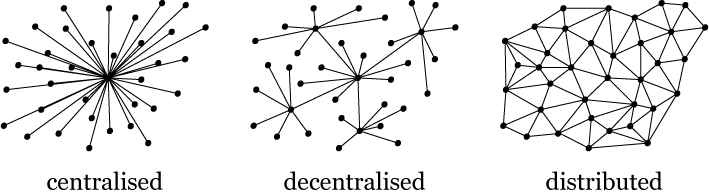
\includegraphics[scale=0.55]{./figures/types-networks2}
  	\caption{Représentation de quelques types de réseaux composés par des nœuds et des liens. }
  	\label{exemples-reseaux}
  \end{figure}
  \subsection{Différents types des Réseaux complexes}
  L'étude des réseaux complexes a été inspirée par le désir de comprendre les différents systèmes réels, allant des réseaux de communications aux réseaux écologiques. Les bases de données empiriques disponibles pour l'étude couvrent plusieurs disciplines, en générale, elles se divisent en quatre grandes catégories: Réseaux Technologique, Réseaux Biologiques, Réseaux Sociaux
  et Réseaux d'Informations.
  \subsubsection{Réseaux Technologique}
  Les réseaux technologiques sont des réseaux artificiels, qui ont grandi au cours du siècle dernier et qui constituent une grande partie de notre société moderne, comme les réseaux électriques, réseaux téléphoniques, réseaux de transports, etc \cite{Pi1965,Am-al2000,Do-al2007,Se-al2003}.
  L'Internet est parmi les exemples les plus connus et les plus largement étudiés des réseaux technologiques (voir Fig.~\ref{Internet}), on peut le définir comme un réseau de données informatiques dans lequel les nœuds sont des ordinateurs et les liens sont des connexions de données physiques entre eux, tels que des câbles à fibres optiques ou des lignes téléphoniques \cite{F-al1999,BC2001}. Il est curieux que, bien que l'Internet est un réseau artificiel, nous ne connaissons pas exactement sa structure, nos meilleures données actuelles sur sa structure proviennent d'études expérimentales.
  \begin{figure}[h!]
  	\centering
  	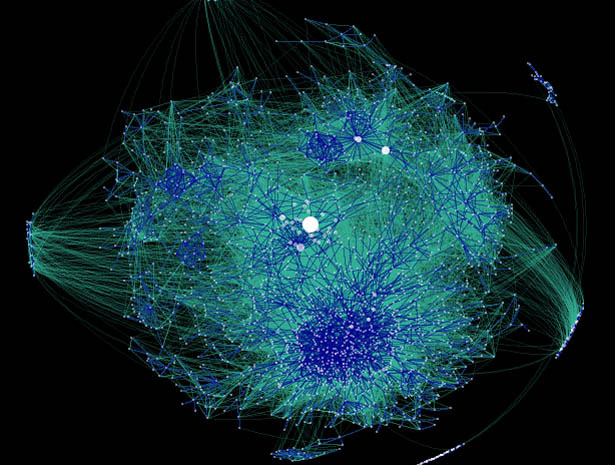
\includegraphics[width=11cm,height=6cm]{./figures/Internet3}
  	\caption{Nous avons ici un affichage hyperbolique de blogs en utilisant à la fois les ensembles de données WWE et ICWSM 2007 (http://datamining.typepad.com/).}
  	\label{Internet}
  \end{figure}

  Il existe un certain nombre d'excellentes raisons pratiques pour être intéressé à étudier la structure du réseau d'Internet, la fonction d'Internet consiste à transporter des données entre ordinateurs dans différentes parties du monde, ce qui se fait en divisant les données en pièces ou en paquets et en les transportant d'un nœud à l'autre sur le réseau jusqu'à ce 
  qu'ils atteignent leur destination, sans aucun doute, la structure du réseau affectera la manière dont il accomplit efficacement cette fonction et si nous connaissons la structure du réseau, nous pouvons aborder de nombreuses questions et problèmes de pertinence pratique.
  
  
  \subsubsection{Réseaux Biologiques}
  Une autre classe des  réseaux les plus étudiées dans la littérature est celle des réseaux biologiques. Cette classe contient une grande variété de réseaux naturels. Le corps, qu'il soit humain ou animal, contient un grand nombre de réseaux, dont certains se produisent dans l'espace réel, tels que le système nerveux. Ces réseaux ont été étudiés depuis longtemps \cite{WB1997}.
  Une autre classe de réseau, ce sont les réseaux d'interactions gène-gène, protéines-gène et protéines-protéines \cite{DM2003}, ainsi que les réseaux d'interactions entre les espèces dans les écosystèmes, comme la prédation ou la coopération.\\
\begin{figure}[h!]
\centering
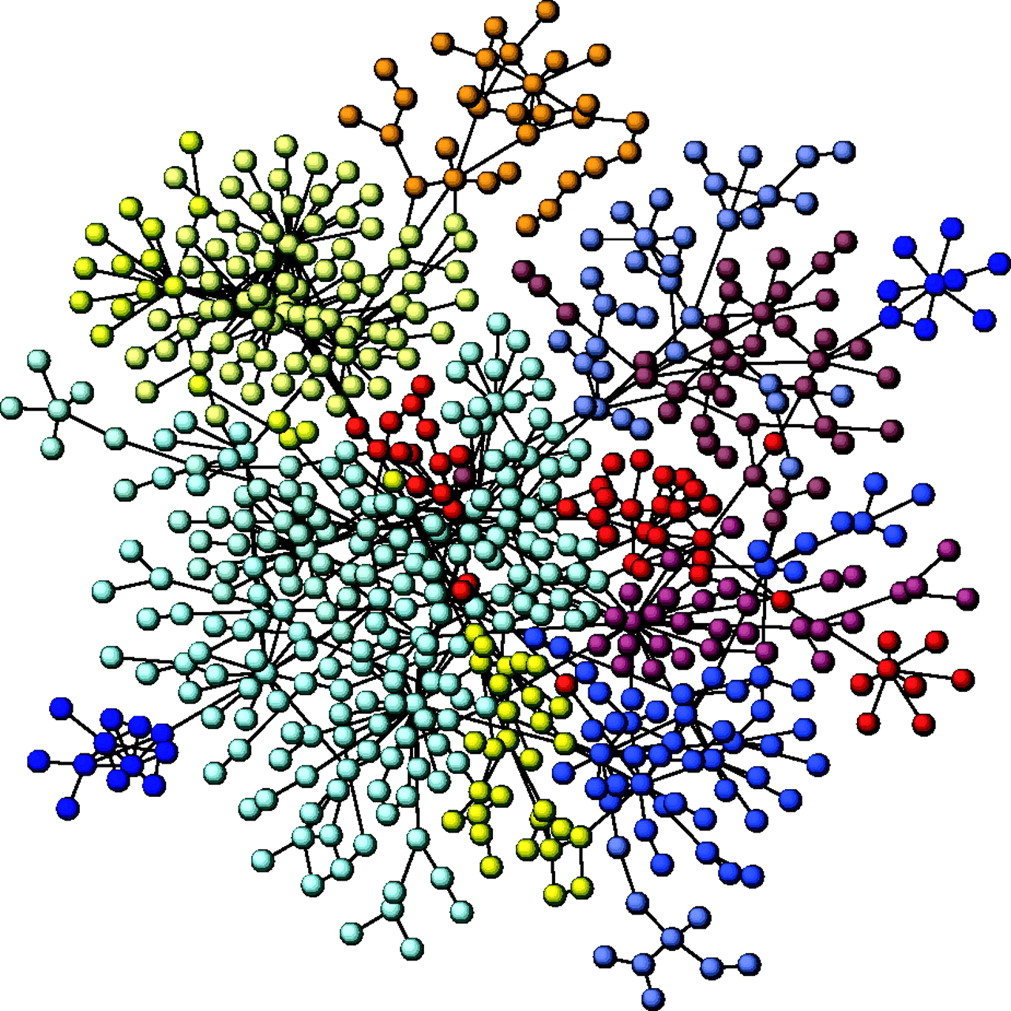
\includegraphics[scale=0.2]{./figures/PPI}
\caption{Un réseau modulaire est illustré au moyen du protéome humain (données obtenues à partir de la base de données DIP: http://dip-doe-mbi.ucla.edu). Les nœuds sont des protéines et des liens indiquent leur interaction physique (protéine-protéine).}
\label{PPI}
\end{figure}
 La structure de ces réseaux se diffère selon chaque cas. Par exemple, les réseaux métaboliques sont des réseaux de protéines interagissant les uns avec les autres à l'intérieur de la cellule Fig.~\ref{PPI}, il s'agit d'un réseau dirigé, car chaque protéine peut catalyser ou réprimer la création d'autres protéines, ce qui n'implique pas nécessairement le processus inverse. La structure à grande échelle des réseaux métaboliques a été étudiée pour de nombreuses espèces, il a été trouvé que ces réseaux ont une distribution des degrés sans-échelle \cite{Je-al2000}. De plus, il a été observé que le diamètre du réseau est très petit et presque indépendant de la taille du réseau, cette indépendance s'explique par que certain classe de réseaux sans-échelle est Ultra-small \cite{Cohen-Havlin2003,Do-al2003,ChL2003}, ainsi que notre résultats du troisième chapitre renforcent cette explication et indiquent que la dépendance du diamètre avec la taille $N$ est très faible.\\ Dans les réseaux génétiques, les nœuds représentent des gènes, et les liens sont dirigés  et représentent l'influence d'un gène sur un autre, le réseau E. coli\footnote{Escherichia coli (en abrégé E. coli) sont des bactéries présentes dans l'environnement, les aliments et les intestins des humains et des animaux. E. coli est un groupe important et diversifié de bactéries.} est un des réseaux génétiques qui est bien étudiés dans la littérature \cite{Mi-al2002}.


  \subsubsection{Réseaux Sociales}
  Un réseau social est un ensemble de nœuds, où ces nœuds se représente par des  personnes  (individus ou groupes sociaux) et les liens par une relation qui peut être de parenté, amitié, statut, etc \cite{JS2000}, cette diversité des liens est une chose appréciée dans l'étude des réseaux sociaux, car il existe de nombreuses définitions possibles d'un tel réseau et la définition particulière que l'on utilisera dépendra des questions auxquelles on est intéressé à répondre. Tel que les réseaux d'amitiés entre les individus \cite{WW1977,Mo1934}, les relations d'affaires entre les entreprises \cite{JP1977}.
  La société offre une grande variété d'organisations de groupes possibles: les familles, les milieux de travail et d'amitié, les villages, les villes, les nations. La diffusion d'Internet a également conduit à la création de groupes virtuels, en direct sur le Web, comme Facebook qui reliant presque tout  notre monde entier (voir Fig.~\ref{Facebook}).
  
\begin{figure}[h!]
\centering
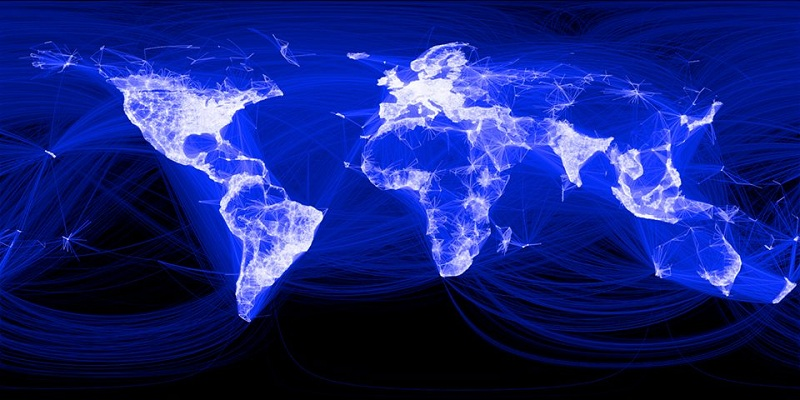
\includegraphics[width=9cm,height=5cm]{./figures/facebook}
\caption{Le graphe social derrière Facebook, graphe des relations d'amis de $500$ million personnes, image par Paul Butley, $2010$.}
\label{Facebook}
\end{figure}
Bien avant que l'Internet commence à jouer un rôle important dans la vie de beaucoup de personnes, les sociologues et d'autres chercheurs des sciences humaines ont examiné la structure des groupes de personnes. Dans la plupart des cas, des groupes relativement petits ont été considérés, nécessairement parce que l'analyse de grands groupes n'était pas souvent possible.\\
Une contribution importante à l'analyse des réseaux sociaux est venue de Jacob Moreno qui a introduit des sociogrammes dans les années $1930$. Un sociogramme peut être considéré comme une représentation graphique d'un réseau: les personnes sont représentées par des points (appelés nœuds) et leurs relations par des lignes reliant ces points (appelés liens).\\
L'analyse des réseaux sociaux a été importante pour le développement ultérieur de la théorie des graphes, par exemple en ce qui concerne l'introduction de mesures pour identifier l'importance des personnes ou des groupes. Par exemple, une personne ayant de nombreuses connexions avec d'autres personnes peut être considérée comme relativement importante. De même, une personne au centre d'un réseau semble être plus influente que quelqu'un au bord. Ce que la théorie des graphes nous fournit, ce sont les outils pour décrire formellement l'importance et l'influence des nœuds. En outre, en utilisant la théorie des graphes, nous pouvons facilement proposer des solutions alternatives pour décrire l'importance des personnes. L'existence de ces outils a également améliorer la précision des déclarations concernant le poste ou le rôle de ces personnes au sein d'une communauté.
  \subsubsection{Réseaux d'informations}        
 Les  réseaux de citation et le World Wide Web (WWW), comme dans Fig.~\ref{WWW}, sont un bon exemple des réseaux d'informations, car leur contenu d'informations étant stockée dans des nœuds, c’est pour cette raison que l’on utilise le terme réseau d’informations. Parfois on rencontre une certaine confusion à propos de réseau  WWW  et le réseau d'Internet. Dans la WWW, les nœuds sont les pages HTML, et les bords représentent les liens entre les pages, par contre  dans l'Internet, les liens correspondent aux câbles physiques entre les ordinateurs. Alors  le WWW est virtuelle et Internet est physique.
\begin{figure}[h!]
	\centering
	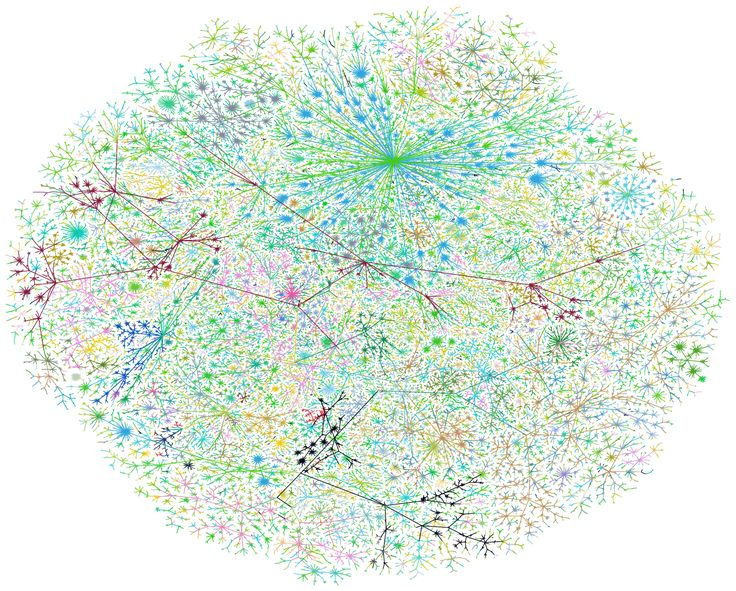
\includegraphics[scale=0.4]{./figures/www2}
	\caption{La structure de l'Internet au niveau des systèmes autonomes. Les nœuds de cette représentation sont des systèmes autonomes et les bords montrent les itinéraires empruntés par les données qui circulent entre eux. La photo a été créée par Hal Burch et Bill Cheswick en 2009.}
	\label{WWW}
\end{figure}

\section{Les réseaux complexes, la physique moderne et l'unification}
La physique explique les phénomènes de la nature en les réduisant à une interaction de lois fondamentales simples. Cette méthode plutôt réussie semble rencontrer certaines difficultés lorsqu'il s'agit des systèmes complexes en général et des réseaux complexes en particulier. Dans ces derniers il reste peu clair s'il existe des lois universelles uniques expliquant une variété de similitudes structurelles et dynamiques trouvées dans de nombreux réseaux réels différents  \cite{K-al2012,BS2009,La-al2009,Li-al2011}. En revanche, l'\textsf{unification} des lois universelles qui paraissaient jusqu'alors complètement séparées sont-elles d'une  origine commune ? c'est ce que les physiciens théoriques rêvent de découvrir. Une telle  \textsf{unification}
va \^{e}tre, sans doute, un grand pas dans notre compréhension de la nature. En outre, l'existence de cette belle idée au cœur de l'unification montre le pouvoir mystérieux que les êtres humains peuvent découvrir derrière les apparences de la nature \cite{Sm1997}.\\

Le réseau causal représentant la structure à grande échelle de l'espace-temps dans notre univers accéléré est un graphe de loi de puissance avec un regroupement fort, similaire à de nombreux réseaux complexes tels que les réseaux Internet, sociaux ou biologiques \cite{K-al2012}. Cette similitude structurelle est une conséquence de l'équivalence asymptotique entre la dynamique de croissance à grande échelle des réseaux complexes et des réseaux causaux. Par conséquent, un intérêt croissant est adressé à l'étude de la gravité quantique à partir de la théorie de l'information et de la perspective des réseaux complexes \cite{Tr2015,Bi-al2015}. Récemment, des relations intrigantes entre les propriétés des réseaux de communication quantique avec des topologies du réseau et la physique statistique ont été rapportées. Sur la base des concepts classiques de percolation \cite{BR2006}, il a été montré que ces réseaux quantiques peuvent présenter une transition de phase de percolation d'enchevêtrement \cite{Ac-al2007,Sa1999}.
L'avancement rapide de la technologie de l'information quantique a suscité un intérêt considérable pour les propriétés dynamiques des réseaux quantiques formés par les systèmes élémentaires, tels que les qubits, en raison de leur rôle privilégié dans la communication et le calcul quantiques \cite{J-al2015,BG2007,MC2000}.\\

Une autre domaine de recherche en relation avec les sciences des réseaux et notamment aux réseaux complexes. La science générale des réseaux et de ses diverses applications a une pertinence significative pour les praticiens de l'intelligence artificiel (IA). Par exemple, la compréhension de la structure d'Internet et du World Wide Web sera importante pour l'orientation de la direction de l'intelligent, l'équilibrage de charge, la recherche de toutes sortes et le déploiement d'agents\footnote{Un agent est un terme important en IA qui désigne une entité capable d’interagir avec
	son environnement.} intelligents qui assistent les utilisateurs dans leurs tâches réseau. La réflexion en réseau sera également fondamentale pour développer des algorithmes décentralisés efficaces pour les réseaux de calcul, de communication et de détection de plus en plus distribués et liés, ainsi que des méthodes de sécurité efficaces pour ces systèmes de plus en plus vulnérables. Ce sont tous des domaines dans lesquels la recherche sur l'IA et l'apprentissage automatique ont joué et joueront un rôle majeur \cite{Mitchell2006,Basheer-Hajmeerb2000,Passerini-al2017}.

\section{La théorie des graphes}
En terme générale, un réseau se décrit comme un graphe dont les nœuds (sommets) identifient les éléments du
système et les liens de connexion (arêtes) représente la présence d'une relation ou d'une interaction entre ces
éléments. Avec un tel niveau de généralité, il est facile de percevoir qu'un large éventail de systèmes peuvent être abordés
dans le cadre de la théorie du graphe. Alors nous fournissons ici un bref historique et quelques notations de base nécessaires
dans la théorie de graphe pour décrire les réseaux. Le cadre naturel pour une description mathématique rigoureuse des réseaux
se trouve dans la théorie des graphes, mais il faut noter que la théorie des graphes 
constitue une branche des mathématiques vaste et compliquée et nous ne sommes pas dans l'état de fournir une présentation formelle et complète de 
celle-ci. Cependant notre but dans ce chapitre d'introduction est de fournir seulement quelques notions utiles pour décrire 
les réseaux dans la suite de cette thèse. Pour les lecteurs souhaitant aller plus en détail dans l'étude de la théorie des graphes pourraient consulter ces livres \cite{Ha1995,West1996}.
  \subsection{Bref historique}
  En plus de la topologie, Euler est devenue le père de la théorie des graphes quand il a résolu, en $1736$, un problème célèbre
sous le nom \textit{"le problème du pont de K\"{o}nigsberg"}, la question était de savoir s'il était possible de visiter les quatre
quartiers de la ville séparés les uns des autres par un bras de rivière, en passant exactement une fois par chaque pont et en 
revenant à son point de départ (voir Fig.~\ref{Konig}).
\begin{figure}[h!]
\centering
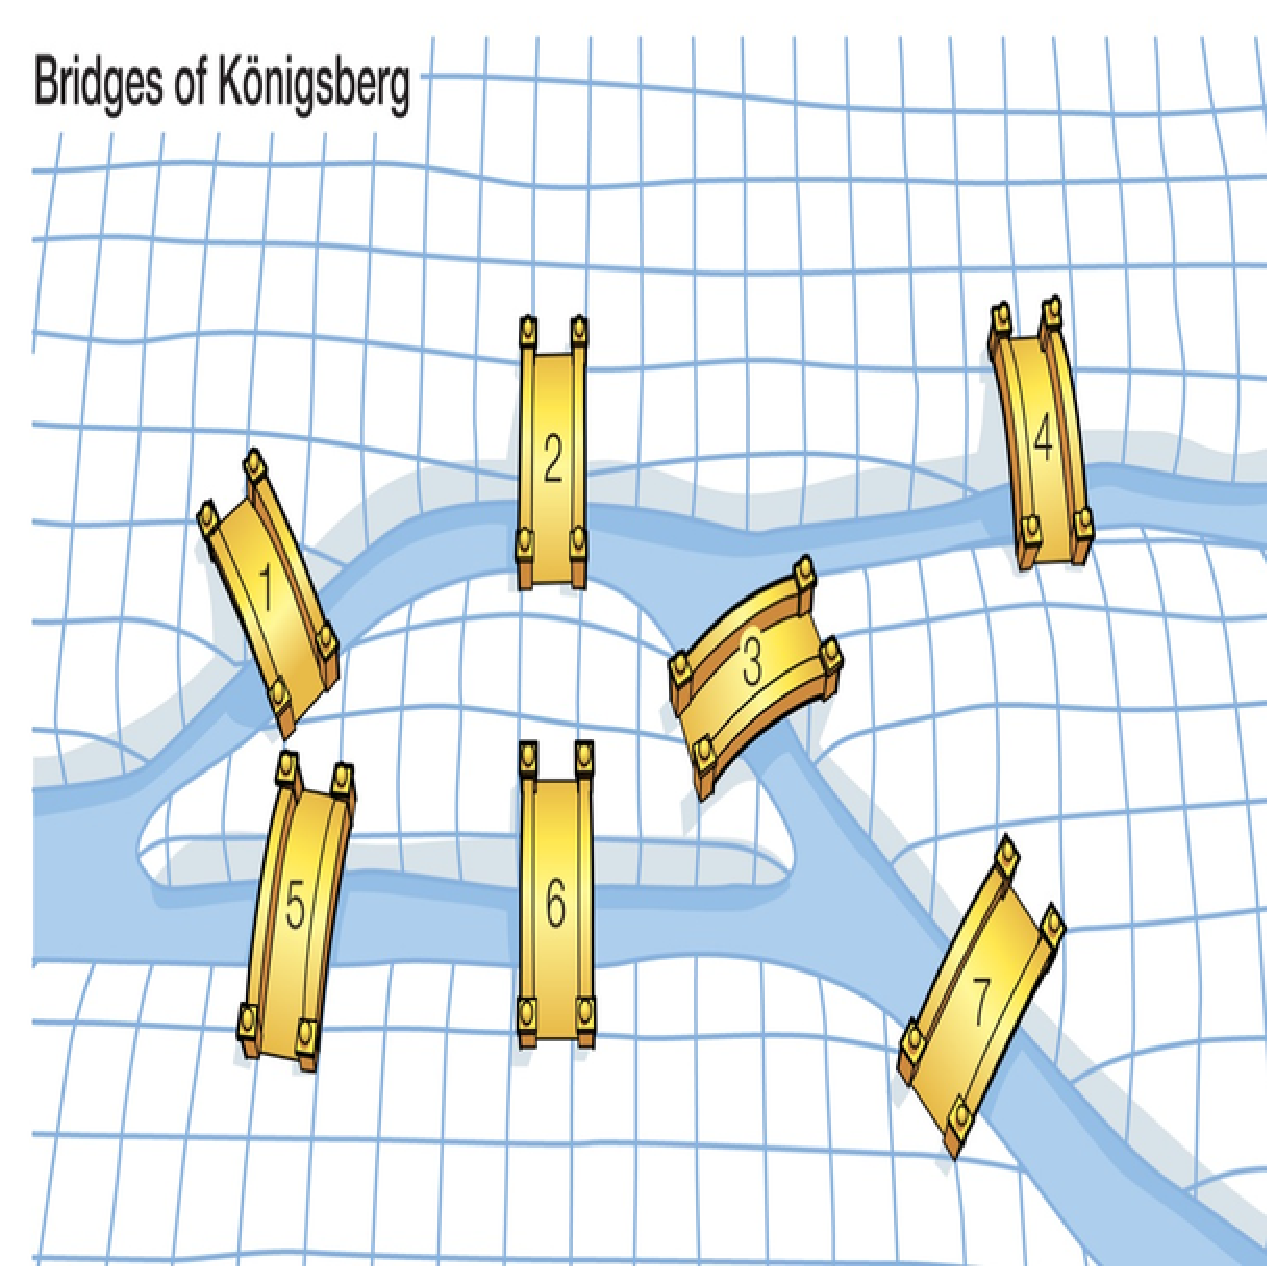
\includegraphics[scale=0.7]{./figures/Konig}
\caption{Ponts de K$\ddot{o}$nigsberg, $1736$}
\label{Konig}
\end{figure}
Afin de trouver une solution à ce problème Euler a remplacé chaque zone de terrain par un point et chaque pont par une ligne 
joignant les points correspondants, produisant ainsi un \textit{"graphe"}. Ainsi il a montré que le problème
est insoluble et que le graphe de cette ville ne peut pas être parcouru d'une certaine manière.

En $1847$ Kirchhoff a développé la théorie des arbres afin de résoudre le système d'équations linéaires simultanées qui 
donnent le courant dans chaque branche et autour de chaque circuit d'un réseau électrique. Bien qu'un physicien, il a pensé comme un mathématicien lorsqu'il a remplacé un réseau électrique par sa structure combinatoire  correspondante constituée uniquement de points et de lignes sans indication du type d'élément électrique représenté par des lignes individuelles.
Dans les années $1960$, deux mathématiciens, Paul Erd\H{o}s et Alfred Rényi (ER), ont introduit une nouvelle idée ingénieuse, ils ont 
combiné les concepts de la théorie des graphes avec les outils de la théorie des probabilités, cela permettant d'envisager des
familles de graphes plutôt que des graphes spécifiques.

  \subsection{L’expérience de Milgram}
 \label{Milgram} 
En $1967$, Stanley Milgram a effectué une expérience intéressante.  Dans sa première expérience, Milgram a demandé à des personnes choisies au hasard au Nebraska d'envoyer des lettres à une personne cible éloignée à Boston.
Les participants ne pouvaient passer que les lettres (à la main) aux connaissances personnelles qu'ils pensaient pouvoir 
atteindre la cible, soit directement, soit via un  "ami d'un ami".  dans sa première experience seules trois lettres ont
finalement atteint leur destination. Mais dans les expériences ultérieures, Milgram a réussi à augmenter
le taux de réussite à $95\%$, pour plus de détails (voir \cite{Mi1967,TM1969}). La conclusion principale du cette expérience
de Milgram était que la plupart des gens sur notre planète n'est séparé que par six autres personnes en moyen. Cette idée de
Milgram a été reprise encore une fois en 2001 par Duncan Watts et ses collègues en utilisant un message électronique qui devait être livré à des expéditeurs autour de monde, étonnamment, Watts a constaté que le nombre moyen d'intermédiaires était
$6$. Pour plus de détails et une analyse statistique beaucoup plus étendue des données par rapport à l'analyse de Milgram,
voir Dodds et al \cite{D-al2003}.

  \subsection{Représentation d'un graphe}
  Comme dans toute abstraction mathématique, lorsque nous décrivons un système en tant que graphe, nous décidons de rejeter  plusieurs des particularités particulières des phénomènes réels et de nous concentrer uniquement sur quelques caractéristiques  d'intérêt. En particulier, un graphe est essentiellement un moyen de coder une relation, liens physiques, interactions,
  etc, entre les éléments d'un système. Les éléments du système identifient l'ensemble $V$ (ensemble des nœuds) et les relations entre ceux de l'ensemble $E$ (ensemble des liens). Le graphe indiqué comme $G(V, E)$ peut être présenté en traçant les  nœuds en tant que points et les bords comme lignes entre eux.\\ 
 
   Parmi les façons de présentation basées sur cette définition on peut citer la matrice d'adjacence et la liste d'adjacence:
  \subsubsection{La matrice d’adjacence}
 Un graphe est représenté fréquemment par une matrice d'adjacence, $M_{i,j}$, dans laquelle chaque ligne et
 chaque colonne représente un nœud du graphe. Dans un graphe non-dirigé l'élément $M_{i,j}=1$ si un lien existe entre le $i^{eme}$ et $j^{eme}$
 nœud sinon $M_{i,j}=0$  (voir Fig.~\ref{matrice d'adjacence}), ainsi la matrice sera en général asymétrique et les éléments diagonaux ne sont pas
 nécessairement $0$.
  \begin{figure}[h]
 	\centering
 	\subfloat{
 		\begin{tikzpicture}[shorten >=1pt,auto,node distance=2cm,thick,main node/.style={circle,fill=black!20,draw}]
 		%[-,>=stealth',shorten >=1pt,auto,node distance=2cm,thick,main node/.style={circle,fill=black!20,draw}]
 		\node[main node] (1) {$v_2$};
 		\node[main node] (2) [below left of=1] {$v_1$};
 		\node[main node] (3) [below right of=1] {$v_3$};
 		\node[main node] (4) [below of=3] {$v_4$};
 		\node[main node] (5) [below of=2] {$v_5$};
 		
 		\path[every node/.style={font=\sffamily\small}]
 		(2) edge node [left] {} (1)
 		(2) edge node [left] {} (3)
 		(1) edge node [left] {} (5)
 		(1) edge node [left] {} (3)
 		(3) edge node [left] {} (4)
 		(4) edge node [left] {} (5)
 		;
 		\end{tikzpicture}}
 	\subfloat{
 		\vbox{\hbox{
 				\begin{math}
 				M_{G} = \left(
 				\begin{array}{ccccc}
 				0 & 1 & 1 & 0 & 0 \\
 				1 & 0 & 1 & 0 & 1 \\
 				1 & 1 & 0 & 1 & 0 \\
 				0 & 0 & 1 & 0 & 1 \\
 				0 & 1 & 0 & 1 & 0
 				\end{array}
 				\right)
 				\end{math}
 			}% end of first hbox
 			\null% last null hbox, which sets the baseline of the \vbox
 		} % end of vbox
 	} % end of subfloat
 	\caption{Exemple d'un graphe non-orienté et sa matrice d'adjacence $M_G$ avec 5 nœuds et 6 liens.}
 	\label{matrice d'adjacence}
 \end{figure}  
 
  Un graphe orienté est un graphe où les bords sont dirigés, c'est-à-dire que chaque bord est une paire de nœuds ordonnée avec ($i$,$j$) désignant un bord (flèche) qui commence au nœud $i$ et se termine au nœud $j$ Fig.~\ref{matrice d'adjacence2}. 
 
 
 \begin{figure}[h]
	\centering
	\subfloat{
		\begin{tikzpicture}[->,shorten >=1pt,auto,node distance=2cm,thick,main node/.style={circle,fill=black!20,draw}]
		%[-,>=stealth',shorten >=1pt,auto,node distance=2cm,thick,main node/.style={circle,fill=black!20,draw}]
		\node[main node] (1) {$v_2$};
		\node[main node] (2) [below left of=1] {$v_1$};
		\node[main node] (3) [below right of=1] {$v_3$};
		\node[main node] (4) [below of=3] {$v_4$};
		\node[main node] (5) [below of=2] {$v_5$};
		
		\path[every node/.style={font=\sffamily\small}]
		(2) edge node [left] {} (1)
		(2) edge node [left] {} (3)
		(1) edge node [left] {} (5)
		(1) edge node [left] {} (3)
		(3) edge node [left] {} (4)
		(4) edge node [left] {} (5)
		;
		\end{tikzpicture}}
	\subfloat{
		\vbox{\hbox{
				\begin{math}
				M_{G} = \left(
				\begin{array}{ccccc}
				0 & 0 & 0 & 0 & 0 \\
				1 & 0 & 0 & 0 & 0 \\
				1 & 1 & 0 & 0 & 0 \\
				0 & 0 & 1 & 0 & 0 \\
				0 & 1 & 0 & 1 & 0
				\end{array}
				\right)
				\end{math}
			}% end of first hbox
			\null% last null hbox, which sets the baseline of the \vbox
		} % end of vbox
	} % end of subfloat
	\caption{Exemple d'un graphe orienté et sa matrice d'adjacence $M_G$ avec 5 nœuds et 6 liens.}
	\label{matrice d'adjacence2}
\end{figure}


\subsubsection{La liste d’adjacence}
Le format de liste d'adjacence est utile pour les graphes sans données associées aux nœuds ni aux bords et à des nœuds
qui peuvent être représentés de manière significative sous la forme de chaînes, il se compose de 
lignes avec des étiquettes de nœud, la première étiquette dans une ligne est le nœud source, les autres étiquettes dans la
ligne sont considérées comme des nœuds cibles et sont ajoutées au graphe avec un bord entre le nœud source et le nœud 
cible.\\
\begin{figure}[h]
	\centering
	\subfloat{
		\begin{tikzpicture}[shorten >=1pt,auto,node distance=2cm,thick,main node/.style={circle,fill=black!20,draw}]
		%[-,>=stealth',shorten >=1pt,auto,node distance=2cm,thick,main node/.style={circle,fill=black!20,draw}]
		\node[main node] (1) {$v_2$};
		\node[main node] (2) [below left of=1] {$v_1$};
		\node[main node] (3) [below right of=1] {$v_3$};
		\node[main node] (4) [below of=3] {$v_4$};
		\node[main node] (5) [below of=2] {$v_5$};
		
		\path[every node/.style={font=\sffamily\small}]
		(2) edge node [left] {} (1)
		(2) edge node [left] {} (3)
		(1) edge node [left] {} (5)
		(1) edge node [left] {} (3)
		(3) edge node [left] {} (4)
		(4) edge node [left] {} (5)
		;
		\end{tikzpicture}}
	\subfloat{
		\vbox{\hbox{
				\begin{math}
				\begin{tabular*}{0.5\textwidth}{@{\extracolsep{\fill}}ccc} \toprule Noueds	& voisins\\ \midrule 1	& 2,3\\ 2	& 1,3\\ 3	& 1,2,4\\ 4	& 3,5\\ 5 & 2,4 \\ \bottomrule
				\end{tabular*}			
				\end{math}
			}% end of first hbox
			\null% last null hbox, which sets the baseline of the \vbox
		} % end of vbox
	} % end of subfloat
	\caption{Exemple d'un graphe non-orienté et sa liste d'adjacence avec 5 nœuds et 6 liens.}
	\label{matrice d'adjacence1}
\end{figure}

En règle générale, les matrices sont utilisées pour les tableaux denses et les listes d'adjacence pour les 
tableaux dispersés. La raison est que les matrices consomment moins d'espace pour les tableaux denses et les listes
d'adjacence consomment moins d'espace pour les tableaux dispersés. Cependant, l'espace n'est qu'une considération, d'autres
facteurs doivent également être pris en compte.


\section{Caractéristiques des réseaux complexes}

On croit que ne comprend pas encore les réseaux de manière appropriée. Par exemple, si les données (la matrice d'adjacence) d'un grand graphe sont présentes et que vous n'êtes pas autorisé à visualiser le réseau,
il semble assez complexe de dire simplement quelles sont les propriétés du réseau. Alors
l'étude de ces réseaux oblige à ajouter d'autres caractéristiques supplémentaires, telles que, le plus court chemin,
Clustering, etc.
   \subsection{Plus court chemin}
   
   Le plus court chemin entre deux nœuds d'un graphe est défini comme étant la longueur du trajet le plus court parmi tous les trajets possibles. Une
   mesure statistique globale de la distance entre les nœuds peut alors être exprimée comme la valeur moyenne des chemins les
   plus courts entre tous les couples possibles de nœuds du réseau, mathématiquement on peut le définir par la forme suivante
   \begin{equation}
    l=\frac{1}{n(n-1)}\sum_{i,j} d_{i,j},
   \end{equation}
   avec $d_{ij}$ est la distance la plus courte du nœud $i$ au nœud $j$ et $n$ est le nombre total de nœuds dans le réseau. Sachant que la distance entre deux nœuds qui ne sont pas atteignables de l'un à l'autre est $0$  et la distance d'un nœud à lui-même est également $0$.\\
   Dans de nombreux réseaux à grande échelle, la distance moyenne entre les nœuds est très faible par rapport à la taille du graphe, ce phénomène est connu sous le nom de la propriété \textit{petit-monde}. Cette propriété a été popularisé dans le contexte sociologique où elle est parfois appelée \textit{six degrés de séparation}\cite{Mi1967}.\\
   L'importance de cette propriété consiste en son rôle important dans le transport et la communication au sein d'un réseau. Supposons qu'il soit nécessaire d'envoyer un paquet de données d'un ordinateur à un autre via Internet: la géodésique fournit un chemin  optimal, car on pourrait obtenir un transfert rapide et conserver les ressources du système \cite{PV2004}. Pour une telle raison, les chemins les plus courts ont également joué un rôle important dans la caractérisation de la structure interne d'un graphe \cite{Wa1994,JS2000,Bo-al2006}.

   Les ensembles de données massifs du réseau s'accumulent à un rythme énorme dans des champs variés \cite{Qi-al2010}. En utilisant la mesure moyenne du plus court chemin, les réseaux de petit-monde peuvent être considérés comme des systèmes à la fois efficaces à l'échelle mondiale et locale \cite{Latora-Marchiori2001}. Nous utilisons souvent la longueur du plus court chemin comme mesure de l'efficacité du réseau, ce qui nous permet de donner une analyse quantitative précise de l'efficacité du flux d'information dans les réseaux. Le calcul du plus court chemin a également été utilisé pour estimer la précision des approximations analytiques de la dynamique sur les réseaux \cite{Melnik-al2011}, en examinant l'apparition de la synchronisation \cite{Zhao-al2006} et en évaluant la résilience des réseaux de communication aux attaques et aux échecs \cite{Albert-al2000}.
   
   \subsection{Coefficient de regroupement (Clustering)}
   En plus de l'effet du petit-monde un haut niveau de regroupement s'en accompagne dans de nombreux
   réseaux sociaux et différents autres réseaux ont montré cette tendance également, notamment le réseau mondial \cite{Lad1999}, les réseaux de transport \cite{Seb-al2022} et les réseaux métaboliques \cite{WD2000,SC2001}.
   Le concept de regroupement d'un graphe
   se réfère à la tendance observée dans de nombreux réseaux naturels à former des cliques au voisinage d'un nœud donné, 
   cette propriété est appelée également la transitivité dans le contexte de la sociologie \cite{Wa1994}.\\
   Le coefficient de regroupement peut être considéré comme la fraction de paires de nœuds avec un nœud commun
   ou équivalent comme la probabilité moyenne que deux nœuds voisins ont un nœud commun, c'est peut-\^{e}tre la manière
   la plus utile de définir le coefficient de regroupement. En notation mathématique:
    \begin{equation}
    C=\frac{3\times\text{(Nombre de triangles)}}{\text{(Nombre de triplets connectés)}}
    \label{Clustering}.
   \end{equation}
   Le facteur $3$ dans le numérateur compense le fait que chaque triangle complet de trois nœuds contribue à trois triplets
   connectés, l'un centré sur chacun des trois nœuds et assure que $0\leq C\leq 1$.
 
 \begin{figure}[h!]
   \begin{center}
   \begin{tikzpicture}
   \tikzset{main node/.style={circle,fill=blue!20,draw,minimum size=0.5cm,inner sep=0pt},
            }
    \begin{scope}[xshift=1.5cm]
    \node[main node] (1) {};
    \node[main node] (2) [right = 1cm  of 1]  {};
    \node[main node] (3) [below = 1cm  of 1] {};
    \node[main node] (4) [right = 1cm  of 3] {};

    \path[draw,thick]
    (1) edge node {} (2)
    (4) edge node {} (3)
    (3) edge node {} (1)
    (4) edge node {} (2);
     \end{scope}
    \begin{scope}[xshift=5cm]
    \node[main node] (1) {};
    \node[main node] (2) [right = 1cm  of 1]  {};
    \node[main node] (3) [below = 1cm  of 1] {};
    \node[main node] (4) [right = 1cm  of 3] {};

    \path[draw,thick]
    (1) edge node {} (2)
    (1) edge node {} (3)
    (3) edge node {} (2)
    (3) edge node {} (4)
    ;
    \end{scope}
    \begin{scope}[xshift=8.5cm]
     \node[main node] (1) {};
    \node[main node] (2) [right = 1cm  of 1]  {};
    \node[main node] (3) [below = 1cm  of 1] {};
    \node[main node] (4) [right = 1cm  of 3] {};
    
    \path[draw,thick]
    (1) edge node {} (2)
    (1) edge node {} (3)
    (1) edge node {} (4)
    (2) edge node {} (3)
    (2) edge node {} (4)
    (3) edge node {} (4)
    ;
    \end{scope}
\node[text width=2cm] at (2.7,-2.2) {$C=0$};
\node[text width=2cm] at (6.1,-2.2) {$C=7/12$};
\node[text width=2cm] at (9.7,-2.2) {$C=1$};
\end{tikzpicture}
\end{center}
   \caption{ Exemple de coefficient de regroupement.}
\label{Clustering}
\end{figure}

Une autre définition du coefficient de regroupement, également largement utilisé, a été donnée par Watts et Strogatz \cite{WS1998},
qui a proposé de définir une valeur locale
 \begin{equation}
    C_i=\frac{\text{(Nombre de triangles connectés au nœud $i$)}}{\text{(Nombre de triples centrés sur le nœud $i$)}}.
  \end{equation}
  Dans le cas où le nœud a le degré $0$ ou $1$, nous mettons $C_i=0$, Ensuite, le coefficient de regroupement pour l'ensemble
  du réseau est la moyenne
  \begin{equation}
    C=\frac{1}{n}\sum_i C_i.
  \end{equation}
 Le coefficient de regroupement mesure la densité des triangles dans un réseau. Une généralisation évidente a été envisagée à 
propos de la densité des boucles plus longues que trois, boucles de longueur quatre et plus. Un certain nombre d'auteurs ont 
examiné ces coefficients de regroupement d'ordre supérieur \cite{Ne2003,BC2003,Fron-al2002,Gle-al2001}, bien qu'il n'y ait jusqu'à présent
aucune théorie propre qui sépare les contributions indépendantes des différents ordres l'un de l'autre.
 %\vspace{2 cm}
   \subsection{Distribution des degrés}
   La propriété la plus importante qui caractérise une structure de réseau est la distribution des degrés $P(k)$,
   définie comme la probabilité qu'un nœud choisi uniformément au hasard ait un degré $k$ ou, de manière équivalente, la
   fraction de nœuds dans le graphe ait le degré $k$.
   Si le graphe est dirigé, le degré du nœud comporte deux composantes: le nombre de liens sortants $k^{out}$ (appelé
   "out-degree") et le nombre de liens entrants $k^{in}$ (appelé "in-degree"). Le degré total est alors défini comme 
   $k=k^{out}+k^{in}$.\\
%   \begin{figure}[h!]
%   	\centering
%   	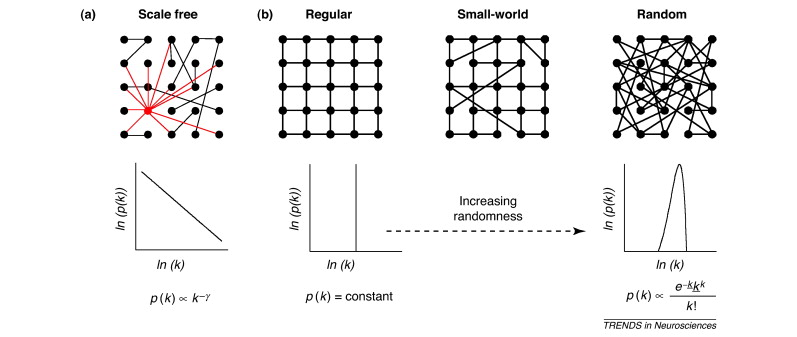
\includegraphics[width=12cm,height=8cm]{./figures/distribution-degree}
%   	\caption{.}
%   	\label{distribution-degree}
%   \end{figure}

Un réseau ordinaire a une séquence de degré simple parce que tous les nœuds ont le même nombre de bords, et donc une forme de distribution des degrés qui contient une seule pointe forte. En outre dans le cas d'un réseau complètement aléatoire, 
la séquence de degré obéit à la distribution de Poisson qui diminue exponentiellement, loin de la valeur moyenne $\textless k\textgreater$. En raison de ce déclin exponentiel, la probabilité de trouver un nœud avec $k$ bord devient négligeable pour  $k\gg \textless k\textgreater$.
Au cours des dernières années, de nombreux résultats empiriques ont montré que pour la plupart des réseaux réels à grande échelle, la distribution des degrés s'écarte de manière significative de la distribution de Poisson.\\
En particulier, pour un certain nombre de réseaux, la distribution des degrés peut être mieux décrite par une loi de puissance de la forme $P(k)\sim k^{-\gamma}$. Cette distribution de la loi de puissance diminue progressivement et permet de créer quelques nœuds de très grande importance. Étant donné que ces lois de puissance sont libres de toute échelle caractéristique, un tel réseau est appelé un réseau sans-échelle.

\subsection{Degré de corrélation} 
Un grand nombre de réseaux réels sont corrélés en sens que la probabilité qu'un nœud de degré $k$ soit connecté à un autre
nœud de degré, disons $k'$, dépend de $k$. Dans ces cas, il est nécessaire d'introduire la probabilité conditionnelle 
$P(k'\backslash k)$, étant défini comme la probabilité qu'un lien d'un nœud de degré $k$ soit connecté à un nœud de degré 
$k'$ \cite{BP2002}. Bien que les corrélations de degré soient formellement caractérisées par $P(k'\backslash k)$, l'évaluation directe de la probabilité conditionnelle donne des résultats extrêmement bruyants pour la plupart des réseaux réels en raison de leur taille finie $N$. Ce problème peut être surmonté en définissant le degré moyen des voisins les plus proches d'un nœud $i$
comme
\begin{equation}
 k_{nn,i}=\frac{1}{k_i}\sum_{j\in N_i}k_j,
\end{equation}
où la somme s'exécute sur les nœuds appartenant à $N_i$ qui signifie l'ensemble des premiers voisins de $i$. on peut calculer le degré 
moyen des voisins les plus proches des nœuds avec le degré $k$, noté $k_{nn}(k)$, obtenant une expression qui intègre implicitement
la dépendance de $k$. Une telle quantité peut, en effet, être exprimée en termes de probabilité conditionnelle comme
\begin{equation}
 k_{nn}(k)=\sum_{k'}k'P(k'\backslash k).
 \label{knn}
\end{equation}
S'il n'y a pas de corrélation de degré, l'équation Eq.~\eqref{knn} donne
$k_{nn}(k)=\frac{\textless k^2\textgreater}{\textless k\textgreater}$, c'est-à-dire que $k_{nn}(k)$ est indépendant de $k$
\cite{Bo-al2006}.\\
\begin{figure}[h!]
	\centering
	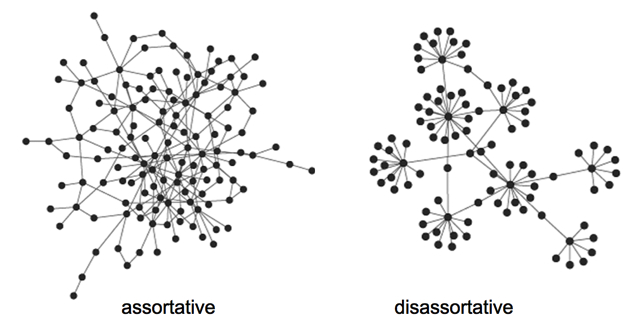
\includegraphics[scale=0.6]{./figures/assortative_disassortative}
	\caption{Exemple des réseaux assortatif et disassortatif.}
	\label{assortative_disassortative}
\end{figure}
\label{s-correl}

Selon l'équation Eq.~\eqref{knn} on peut distinguer deux différents types de réseaux, si les nœuds de haut degré dans un réseau  s'associent préférentiellement avec d'autres nœuds à haut degré on dit que le réseau est assortatif, et s'ils préfèrent  s'attacher à ceux à faible degré on dit que le réseau est disassortatif (voir Fig.~\ref{assortative_disassortative}). Les deux situations sont observées dans certains réseaux, mais le cas du réseau assortatif est particulièrement intéressant, car le degré est lui-même une propriété de la topologie des graphes, alors les corrélations de degré peuvent donner lieu à des effets de structure du réseau intéressants \cite{MS2002,Ne2003}. 

\subsection{Mesures de la centralité}

L'identification des nœuds importants dans les réseaux est un problème intéressant qui a suscité beaucoup d'attention, surtout dans le contexte des réseaux de communication. Par exemple, la communication entre un groupe d'humains forme un réseau de communication \cite{Dehmer2011}. Les sciences sociales à la fin des années 1940 ont développé des mesures théoriques pour détecter des nœuds importants dans les réseaux. Une classe importante de ces mesures est basée sur le concept de centralité \cite{Hage-Harary1995,Wasserman-Faust1994} qui tente intuitivement d'identifier les nœuds qui sont au centre de la communication au sein du réseau parmi tous les nœuds. Il existe deux types fondamentalement différents de mesures de centralité \cite{Freeman1977}. Le premier type évalue la centralité de chaque nœud dans un réseau et s'appelle des mesures de centralité des points où le mot "point" se réfère à un nœud ou un sommet. Le second type s'appelle les mesures de centralité des graphes car il attribue une valeur de centralité à l'ensemble du réseau. Parmi les paramètre du mesure de centralité on cite:\\

%\subsubsection{Centralité d'intermédiarité (Betweenness)}
\begin{itemize}
 \item[i)] Centralité d'intermédiarité (Betweenness):\\
  L'importance d'un nœud dans un réseau dépend de nombreux facteurs. Un site Web peut être important en raison de son contenu, d'un routeur pour sa capacité, d'un métabolite dû à sa fonction biochimique, etc. Bien sûr, toutes ces propriétés dépendent de la nature du réseau étudié et peuvent avoir très peu à faire avec la structure graphique du réseau. L'une des définitions les plus acceptées de centralité est basée sur les chemins de comptage traversant un nœud $i$ dans le réseau, on compte le nombre de chemins de "routage" vers tous les autres nœuds passant par $i$, et ce nombre détermine la centralité $i$. La sélection la plus courante ne prend que les chemins les plus courts en tant que chemins de routage. Cela conduit à la définition suivante: la centralité de l'intermédiarité d'un nœud $i$ équivaut au nombre de chemins les plus courts entre toutes les paires de nœuds dans le réseau qui l'entoure, c'est-à-dire,
 \begin{equation}
 C_B(i)=\sum_{l\neq j}\dfrac{\sigma_{lj}(i)}{\sigma_{lj}},
 \end{equation}
 
 avec $\sigma_{lj}$ indique le nombre des plus court chemins de $l$ à $j$, et $\sigma_{lj}(i)$ indique le nombre des plus court chemins de $l$ à $j$ passant par $i$.
 
%\subsubsection{La centralité de proximité}
\item[ii)] La centralité de proximité:\\
La centralité de proximité tente de mesurer la proximité d'un nœud avec d'autres nœuds du réseau. Ceci se fait en termes de distance de communication mesurée par le nombre d'arêtes entre deux nœuds si connecté par le chemin le plus court.
\begin{equation}
C_C(i)=\dfrac{1}{\sum_{j=1}^nd_{ji}},
\end{equation}
$d_{ji}$ est le plus court chemin entre le nœud $j$ et $i$.

En ce qui concerne la centralité de proximité, les gens se réfèrent généralement à sa forme normalisée qui représente la longueur moyenne des chemins les plus courts au lieu de leur somme. Il est généralement donné par la formule précédente multipliée par $n-1$. Pour les larges réseaux de très grand nombre de nœuds on écrit:
\begin{equation}
C_C(i)=\dfrac{n}{\sum_{j=1}^nd_{ji}}.
\end{equation}
\end{itemize}

\section{Propriétés des réseaux réels}
\subsection{La propriété petit-monde}
La propriété petit monde se réfère au fait que dans plusieurs réseaux, peut-être la plupart des réseaux à grande échelle, la distance moyenne entre les nœuds est très faible par rapport à la taille des graphes. La distance entre deux nœuds d'un graphe est mesurée comme la plus petite longueur de chemin entre eux. Une mesure statistique globale de la distance entre les nœuds peut alors être exprimée comme la longueur moyenne des trajets  les plus courts pour tous les couples possibles de nœuds dans le réseau. Nous avons discuté dans la Section.~\ref{Milgram} l'expérience de Stanley Milgram réalisée dans les années $1960$, dans laquelle on a trouvé que le nombre d'étapes pour qu'un destinataire reçoit la lettre de l'expéditeur, via le réseau social, est égale à six en moyenne. L'expérience de Milgram est une démonstration simple, magnifique et puissante de l'effet de petit-monde.\\
L'effet petit-monde a des implications évidentes pour la dynamique des processus qui se déroulent sur les réseaux. Par exemple, si l'on considère la diffusion de l'information, ou encore tout autre chose, à travers un réseau, l'effet petit-monde implique que cette propagation sera rapide sur la plupart des réseaux réels. Cela affecte le nombre de "sauts" qu'un paquet doit faire pour passer d'un ordinateur à l'autre sur Internet, le nombre d'escales d'un voyage pour un voyageur aérien ou en train, le temps qu'il faut pour qu'une maladie se propage dans
une population, et ainsi de suite. L'effet petit-monde atteint également certains jeux de société bien connus, en particulier le calcul des nombres d'Erd\H{o}s \cite{RG1999} et de Bacon.

\subsection{La distribution des degrés sans-échelle}
\label{s-libre-echelle}
La distribution des degrés sans-échelle qu'on appelle également la loi de puissance a suscité un intérêt particulier au cours des dernières années pour ses propriétés mathématiques, ce qui entraîne parfois des conséquences physiques surprenantes et son apparence dans la diversité des réseaux naturels et artificiels, voir quelques exemples dans la Fig.~\ref{scal-free-reels}.\\

\begin{figure}[h!]
\centering
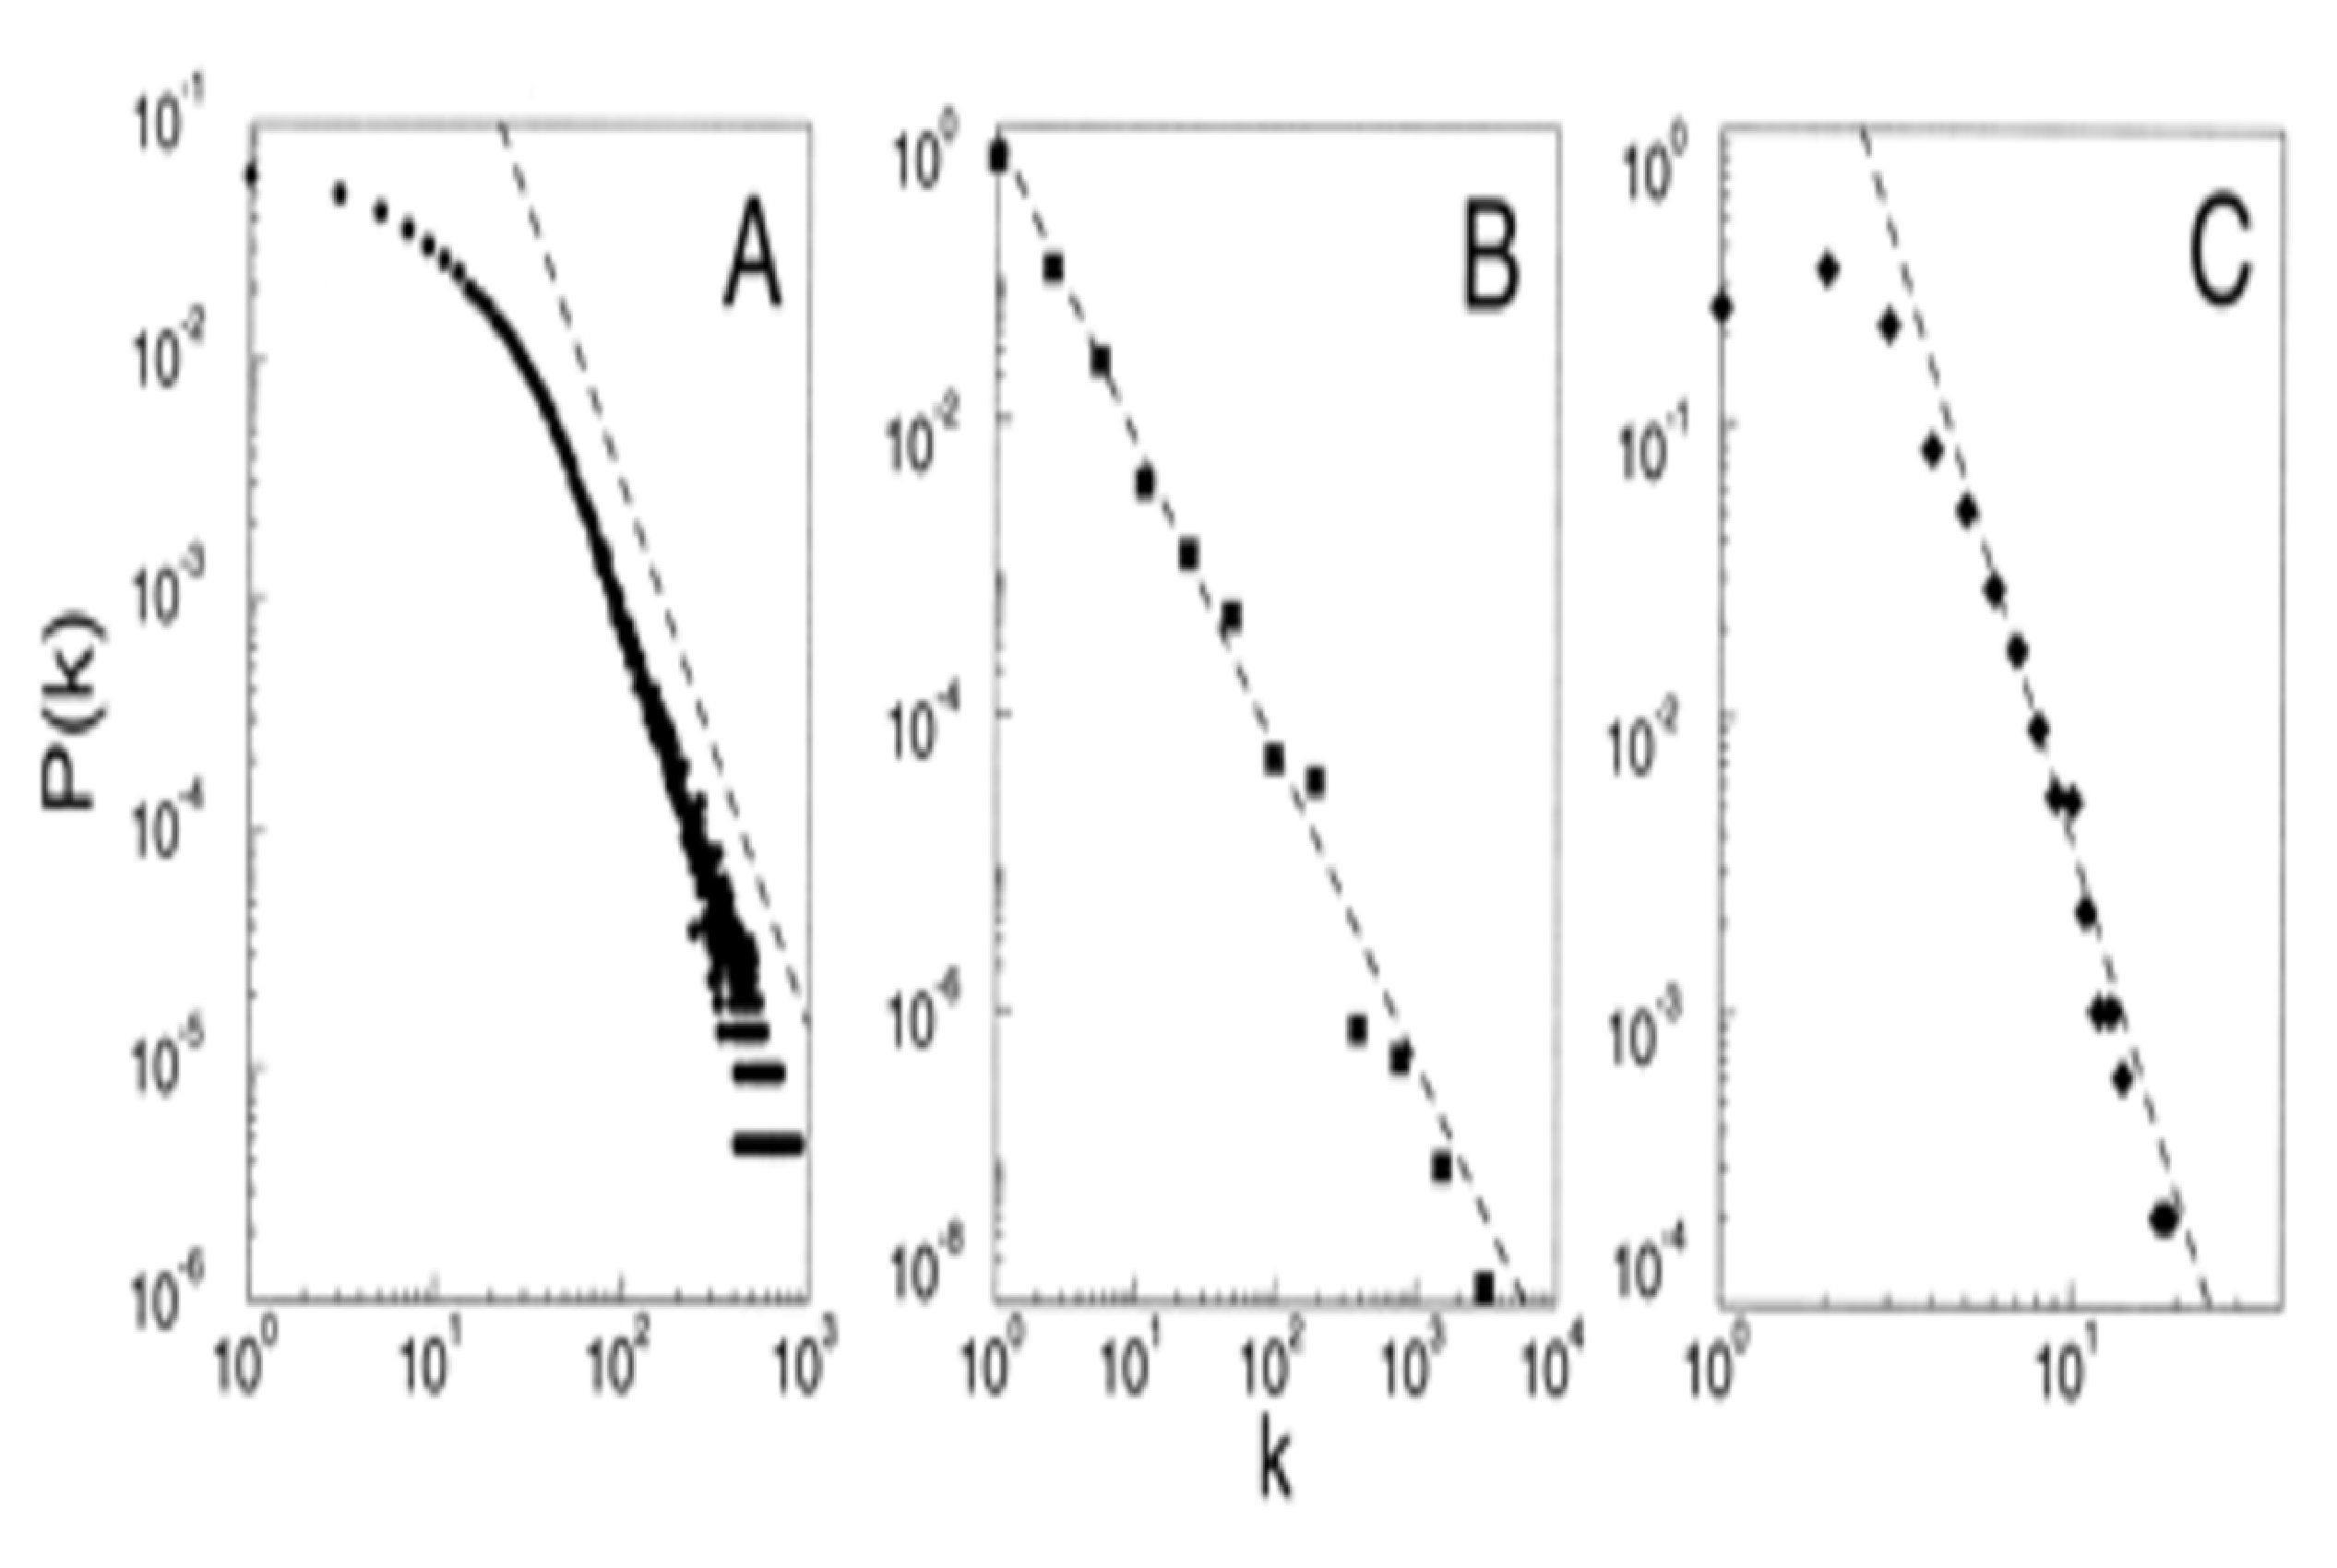
\includegraphics[scale=0.3]{./figures/scal-free-reels}
\caption{Quelques exemples des réseaux sans-échelle, (\textbf{A}) Graphe de collaboration d'acteur avec un nombre des nœuds
$n=212250$ et un degré moyen $\textless k\textgreater=28.78$, (\textbf{B}) WWW, $n=325729$, $\textless k\textgreater=5.46$,
(\textbf{C}) Données du réseau électrique, $n=4941$ et $\textless k\textgreater=2.69$. Les lignes pointillées ont des pentes
(\textbf{A}) $\gamma_{actor}=2.3$, (\textbf{B}) $\gamma_{www}=2.1$ et (\textbf{C}) $\gamma_{electrique}=4$.}

\label{scal-free-reels}
\end{figure}
Les distributions de la loi de puissance se produisent dans une gamme de réseaux extraordinairement diversifiée, tels que, les populations des  villes \cite{New2005,Aa-al2009}, la taille des tremblements de terre \cite{GuR1944}, des cratères de la lune  \cite{NeI1994}, la fréquence d'utilisation des mots dans n'importe quelle langue humaine \cite{Zipf1949,Estoup1916}, la  fréquence de l'apparition de noms personnels dans la plupart des cultures \cite{ZaM2001}, le nombre de documents scientifiques écrits \cite{LoW1926}, le nombre de citations reçues par les documents \cite{Price1965}, le nombre de visites sur les pages Web \cite{AdH2000}, les ventes de livres, les enregistrements musicaux et presque tous les autres produits de marque \cite{Cox-al1995}, le nombre d'espèces dans les genres biologiques \cite{WilY1922}, les revenus annuels des personnes \cite{Pareto1896}, les collecteurs de réseaux quantiques complexes \cite{BiR2015} et une foule d'autres réseaux suivent toutes des distributions de loi de puissances.\\

Mathématiquement, une quantité $x$ obéit à une loi de puissance s'elle est tirée d'une distribution de probabilité
\begin{equation}
 P(x)\propto x^{-\gamma}
\end{equation}
Avec $\gamma$ est un paramètre constant de la distribution connue sous le nom d'exposant, empiriquement cet exposant se situe
généralement dans l'intervalle $2<\gamma<3$, bien qu'il existe des exceptions occasionnelles.

\subsection{Structure communautaire}
La société offre une grande variété d'organisations de groupes possibles: les familles, les milieux de travail et d'amitié, les villages, les villes, les nations (voir un exemple Fig.~\ref{community-network}). La diffusion d'Internet a également conduit à la création de groupes virtuels directement sur le Web. Ces communautés se forment également dans de nombreux systèmes en réseau, de la biologie, de l'informatique, de l'ingénierie, de l'économie, de la politique, etc. Par exemple dans le graphe du World Wide Web les communautés peuvent correspondre à des groupes de pages portant sur les mêmes sujets ou des sujets connexes \cite{Dou-al2007,Flak-al2002}. Dans les réseaux d'interactions protéines-protéines, les communautés sont susceptibles de regrouper des protéines ayant la même fonction spécifique dans la cellule \cite{ChY2006,RivT2003}.\\

\begin{figure}[h!]
	\centering
	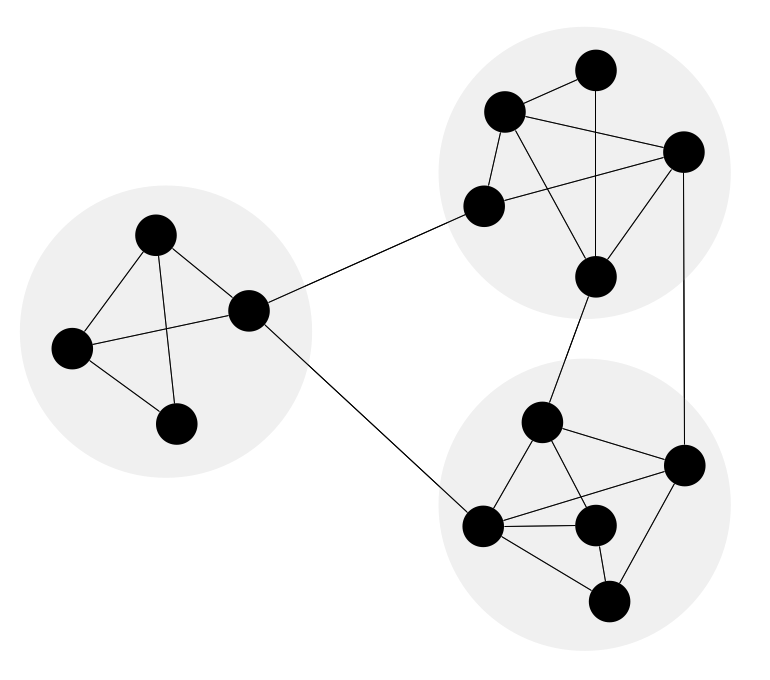
\includegraphics[scale=0.25]{./figures/Network-Community-structure2}
	\caption{Exemples d'un réseau communautaire, on voit trois groupes où chacun est plus connecté par rapport au reste du réseau.}
	\label{community-network}
\end{figure}

Les communautés peuvent avoir des applications concrètes. Le Clustering des clients Web qui ont des intérêts similaires et qui sont géographiquement proches les uns des autres peut améliorer la performance des services fournis sur le WWW, en ce sens chaque groupe de clients pourrait être servi par un serveur miroir dédié \cite{KriW2000}.
Les réseaux auto-configurés formés par des nœuds de communication agissant dans la même région et changeant rapidement, ils n'ont généralement pas de tables de routage centralisées qui spécifient comment les nœuds doivent communiquer entre eux.
Dans ce cas le regroupement des nœuds en clusters permet de générer des tables de routage compactes et rend le choix des chemins de communication plus efficace \cite{Steen2001}.\\
La détection communautaire est également importante pour d'autres raisons. L'identification des modules et de leurs limites permet une classification des nœuds, en fonction de leur position structurelle dans les modules. Donc, les nœuds avec une position centrale dans leurs grappes partagent un grand nombre des liens avec les autres partenaires du groupe, ce qui est une caractéristique importante de contrôle et de stabilité au sein du groupe, en outre, Les nœuds situés aux frontières entre les modules jouent un rôle important de médiation et mènent les relations et les échanges entre les différentes communautés \cite{Csermely2008}.

\section{Les modèles théoriques les plus connus} 
Dans cette section, nous citons les modèles théoriques les plus connus et les plus étudiés, en se limitant principalement à des réseaux non pondérés et non orientés, cependant, la plupart des réseaux présentés peuvent être généralisés facilement. Ces modèles se caractérisent chacun par la manière dont les réseaux sont crées et par plusieurs statistiques résultantes, telles que la distribution des degrés, le plus court chemin entre les nœuds et le coefficient de Clustering.

\subsubsection{Réseaux simples}
Un réseau simple consiste des connexions régulières entre les nœuds. L'un des exemples les plus exceptionnel est le réseau à deux dimensions, comme le montre la Fig.~\ref{Ising2}. Ici, chaque nœud est connecté à ses voisins les plus proches. Malgré sa simplicité, de tels réseaux ont été largement utilisés, par exemple en physique, pour étudier des phénomènes tels que le ferromagnétisme avec le modèle d'Ising \cite{Chowdhury-Stauffer2000}. D'autres exemples de cette classe sont les chaînes linéaires ou les réseaux non rectangulaires tels qu'utilisés, par exemple, dans le contexte de la prédiction de la structure des protéines pour modéliser le repliement des protéines \cite{Hsu-al2003,Dehmer2011}.
\begin{figure}[h!]
	\centering
\begin{tikzpicture}
\clip (-1,-1) rectangle (6cm,5cm); 
\draw[style=help lines,thick] (0,0) grid[step=.5cm] (5,4);

\foreach \x in {0,1,...,10}
{
	\foreach \y in {0,1,...,8}
	{
		\node[draw,circle,inner sep=2pt,fill] at (.5*\x,.5*\y) {};
	}
}
\end{tikzpicture}
\caption{Simple réseau régulier de deux dimensions}
\label{Ising2}
\end{figure}
\subsubsection{Réseaux aléatoires}
Les réseaux aléatoires ont été largement étudiés par Erdös et Rényi (ER) \cite{Erdos-Renyi1959,Erdos-Renyi1960,Erdos-Renyi1961}.
Un graphe aléatoire avec $n$ nœuds est obtenu en connectant chaque paire de nœuds avec la probabilité $p$. Le nombre attendu d'arêtes pour un réseau (non orienté) construit
de cette façon est $E=p\frac{n(n-1)}{2}$.
\subsubsection{Réseaux petit-monde}
Mathématiquement, l'effet de petit-monde décrit les graphes dont le diamètre et la longueur moyenne de la trajectoire croissent beaucoup plus lentement que le nombre de nœuds $n$, typiquement en tant que $\ln n$, comme dans un graphe aléatoire ER. Pourtant, un graphe aléatoire a une très faible interconnexion locale, coefficient de regroupement. Watts et Strogatz \cite{Watss-Strogatz1998} ont réalisé un modèle qui rejoindre la propriété petit-monde et un coefficient de regroupement fort. Le modèle commence par placer tous les nœuds en cercle, puis connecter chaque nœud à ses premiers $k$ voisins les plus proches et en fin avec une probabilité $p$ en prenant chaque lien du réseau et on le reconnecte aléatoirement entre deux autres nœuds.
\subsubsection{Réseaux sans-échelle}
Ni les réseaux aléatoires ni les réseaux petit-monde ont la propriété sans-échelle des degrés, qui est fréquemment observée dans les réseaux du monde réel. Pour expliquer cette caractéristique, Barab\'{a}si et Albert ont introduit un modèle maintenant connu sous le nom de Barab\'{a}si-Albert (BA) \cite{BA1999} ou modèle d'attachement préférentiel qui aboutit à des réseaux sans-échelle qui ont une distribution des degrés suivant une loi de puissance, $P(k)\sim k^{-\gamma}$. La différence majeure entre le modèle d'attachement préférentiel et les autres algorithmes décrits ci-dessus pour générer des réseaux aléatoires ou de petit-monde, est que le modèle d'attachement préférentiel ne suppose pas un nombre fixe de nœuds $n$ et commence alors à les rebrancher avec une probabilité fixe avec d'autres nœuds.

\newcommand{\kms}{\textless k_s(t) \textgreater}
\newcommand{\kmss}{\textless k_s^2(t) \textgreater}

\chapter{Les réseaux en croissances et l'attachement préférentielle}

Malgré de nombreux efforts, la théorie cohérente des réseaux en évolution manque encore un principe général prédisant la topologie d'un réseau formé. Dans le but de comprendre la formation et l'évolution des réseaux complexes, de nombreux modèles ont été introduits pour étudier les processus microscopiques impliqués dans la structure du réseau qui en résulte. Dans ce contexte, on introduit ici un modèle de réseau simple et complexe qui augmente avec un mécanisme linéaire d'attachement préférentiel et sans le mécanisme "rich get richer".
L'objectif est double: d'abord vérifier si la distribution de degré en loi de puissance reste en l'absence du mécanisme "rich get richer" et, d'autre part, voir pour éventuellement les différences microscopiques entre les réseaux sans échelle et homogènes. 

\section{Introduction}

Au cours des dernières années, il existe un intérêt croissant à étudier l'évolution des réseaux complexes et à développer des modèles qui reflètent certaines propriétés des réseaux réels en utilisant les techniques de mécanique statistique, la théorie graphique et les simulations informatiques \cite{BA1999,AB2002,Dorogovtsev-Mendes2002,Newman2003}. L'une des propriétés les plus importantes étudié en réseaux est la distribution de degrés des nœuds qui est la probabilité $P(k)$ qu'un nœud avoir un degré $k$.
On peut distinguer trois lois principales de la distribution de degrés: loi de Poisson où $P(k)=e^{-\langle k\rangle}\frac{\langle k\rangle^k}{k!}$, loi de puissance avec $P(k)\approx k^{-\gamma}$ et $\gamma$ représente le degré d'exposant, et loi exponentiel $P(k)\approx e^{-\frac{k}{c}}$ où $c$ est une constante.\\
Il semble que, dans la nature, la plupart des réseaux suivent les deux dernières lois de distribution mentionnées ci-dessus. Barab\'{a}si-Albert (BA) a réinventé le réseau de distribution de degré libre-échelle de Pric en introduisant un modèle simplifié basé à la fois sur la croissance et l'attachement préférentiel. Le réseau libre-échelle est largement observé dans une variété de systèmes tels que des réseaux de citation de publication, de nombreux réseaux sociaux, des réseaux de protéines et de gènes. Cependant, il existe d'autres réseaux réels qui suivent une loi exponentielle, par exemple, le Réseau mondial de transport maritime \cite{ Deng-al2009}, le réseau nord-américain Power Gridc \cite{Albert-al2004}, réseaux neuronaux des C.elegans \cite{Achacoso-Yamamoto1992} et le réseau de messagerie à l'Université de Rovira i Virgili (ENURV ) en Espagne \cite{Albert-al2004}.\\
La loi exponentielle semble être le résultat d'un réseau croissant en ajoutant de nouveaux nœuds et liens aléatoire. D'autre part, la loi de puissance semble apparaître lorsque les nœuds sont ajoutés au réseau un à la fois et sont liés à des nœuds déjà bien connectés.
De nombreuses idées sur la formation des réseaux ont été examinées. Par exemple, Barab\'{a}si, dans son modèle, a affirmé que l'attachement préférentiels et la croissance sont tous les deux nécessaires pour générer un réseau libre-échelle \cite{BA-al1999}. En réalité, il semble que la croissance n'est pas nécessaire pour un tel objectif \cite{Xie-al2008}. En outre, il est intuitif, que l'attachement préférentiel sans l'effet "rich get richer" ne génère pas un réseau libre-échelle \cite{Samalam}. Krapivsky et al \cite{Krapivsky-al2000} ont étudié la fixation préférentielle non linéaire avec $\Pi(k_i)\varpropto k^{\gamma}$ et ils ont montré que pour $\gamma<1$, le mécanisme produit une distribution de degré de loi exponentiel.

\section{Les processus dynamiques: théorie et simulation}

\subsection{Introduction}

Cette section est destiné à  donner une brève introduction à la théorie et à la modélisation des processus d'équilibre et non équilibrés sur les réseaux et à définir les approches et techniques de base de la modélisation utilisées dans la théorie des processus dynamiques. En particulier, on défini le formalisme de l'équation maîtresse et on distingue les phénomènes d'équilibre et de non-équilibre. Malheureusement, même si l'équation maîtresse permet une distinction et une catégorisation conceptuelles importantes, sa solution complète n'est pas assez simple même pour des processus dynamiques très simples. Pour cette raison, on présent au lecteur des techniques qu'on va utiliser au long de cette thèse, telles que les approximations déterministes du champ moyen, qui représentent habituellement des approches pour comprendre les caractéristiques fondamentales du processus étudié. On discute également des approches de modélisation basées sur des outils de Monte Carlo qui sont généralement implémentées dans des méthodes de simulation numérique à grande échelle.\\ 

Le but de ces différentes méthodes théoriques est à fournir un cadre général pour démontrer comment les interactions microscopiques entre les éléments du système conduisent à des phénomènes coopératifs et des propriétés émergentes des processus dynamiques. Cette stratégie, allant de l'interaction microscopique aux phénomènes collectifs émergents, a ses racines dans la méthodologie de la physique statistique et la dynamique de la population, et est actuellement considérée comme un paradigme général pour combler l'écart entre les propriétés locales et les propriétés à grande échelle des systèmes complexes. Il est important de souligner que cette présentation est une grandement abrégée d'un énorme domaine de recherche et ne fait que rayonner la surface de la théorie statistique des processus dynamiques. Les lecteurs intéressés qui veulent plonger dans les subtilités mathématiques et formelles du sujet devraient se référer à des manuels classiques tels que ceux de Ma (1985), Chandler (1987), Huang (1987) et Balescu (1997).
\subsection{Équation maîtresse}
 
 
 
 
Le nom "équation maîtresse" a été inventé à l'origine par Nordsieck, Lamb et Uhlenbeck \cite{Nordsieck-al1940} dans leur étude du modèle Furry des averses de pluie cosmiques \cite{Furry1937}. Peu de temps auparavant, Feller a appliqué une équation de la même structure à la croissance des populations \cite{Feller1939} et Delbrück à des réactions chimiques auto-catalytiques bien mélangées \cite{Delbruck1940}. Pour plus des détailles vous pouvez voire ces références \cite{Kampen2007,Gardiner2009,Weber-Frey2017}.\\
Deux schémas de modélisation principaux sont adoptés pour traiter les processus dynamiques sur les réseaux. Dans le premier, nous identifions chaque nœud du réseau avec un seul individu ou élément du système. Dans le second cas, nous considérons les entités dynamiques telles que les personnes, les paquets d'information, l'énergie ou la matière circulant dans un réseau dont les nœuds identifient les endroits où transitent les entités dynamiques. Dans les deux cas, cependant, la description dynamique du système peut être obtenue en introduisant pour chaque nœud $i$ la notion de variable correspondante $\sigma_i$ caractérisant son état dynamique. Si chaque nœud représente un seul individu, la variable $\sigma_i$ peut décrire un attribut particulier de l'individu.
Sans perdre de généralité, nous pouvons énumérer tous les états possibles $\sigma_i=1, 2,. . ., m$ pour chaque nœud, et la connaissance de la variable d'état de tous les nœuds du réseau définit donc l'état microscopique de l'ensemble du système. Alors on peut désigner une configuration particulière du réseau à l'instant $t$ par l'ensemble $\sigma(t)=[\sigma_1(t),\sigma_2(t),\sigma_3(t), ...,\sigma_N(t)]$, où l'indice $i = 1,. . ., N$ parcourt tous les nœuds du réseau de taille $N$.\\
L'évolution dynamique du système est simplement donnée par la dynamique de la configuration $\sigma(t)$ dans l'espace des phases du système, définie par toutes les configurations possibles. Le processus dynamique est décrit par les transitions d'une état $\sigma^a$ vers une autre état $\sigma^b$. En général, il est impossible de suivre la dynamique microscopique des systèmes à grande échelle en raison du grand nombre de variables et de la nature stochastique de la plupart des phénomènes. Pour cette raison, la description dynamique de base du système repose sur l'approche de l'équation maîtresse (EM) que nous allons brièvement introduire.\\
L'approche EM se concentre sur l'étude de la probabilité $P(\sigma,t)$ de trouver le système à l'instant t dans une configuration donnée $\sigma$. Cette probabilité doit être normalisée, $\sum_{\sigma}P(\sigma,t)=1$, et fournit une description probabiliste du système qui donne les informations les plus pertinentes
\begin{equation}
\frac{\partial P(\sigma,t)}{\partial t}=\sum_{\sigma'}[P(\sigma',t)W(\sigma'\rightarrow \sigma)-P(\sigma,t)W(\sigma\rightarrow \sigma')],
\end{equation}
où la somme s'exécute sur toutes les configurations possibles $\sigma$ et les termes $W(\sigma'\rightarrow \sigma)$ représentent les taux de transition de la configuration $\sigma'$ vers la configuration $\sigma$ en raison de la dynamique microscopique du système.\\ 
Les EM et les simulations basées sur des équations maîtresses sont maintenant utilisées dans de nombreux domaines de recherche. Ils sont appliqués dans les contextes de la dynamique de spin \cite{Glauber1963,Kawasaki1966-1,Kawasaki1966-2,Kawasaki1966-3}, des réseaux régulateurs de gènes \cite{Walczak-al2009,Rao-al2002,Tsimring2014}, de la propagation des maladies \cite{Bailey1950,Rock2014}, de l'homéostasie épidermique \cite{Clayton-al2007}, et les processus sociaux et économiques \cite{Weidlich-Braun1992}. Les processus de file d'attente sont souvent modélisés en termes d'EM, mais dans ce contexte, les équations sont généralement appelées équations de Kolmogorov \cite{Gross-al2008}. 

\subsection{Modélisation et simulations numériques}
La simulation numérique a commencé dans les années cinquante lorsque les ordinateurs ont été utilisés pour la première fois à des fins pacifiques, en particulier, l'ordinateur MANIAC a commencé en 1952 à Los Alamos. La simulation fournit une approche complémentaire aux méthodes théoriques. Les domaines de la physique où les approches perturbatives sont efficaces (gaz dilués, vibrations dans les solides quasi-harmoniques) ne nécessitent pas de méthodes de simulation. Inversement, la physique des états liquides, où peu de résultats exacts sont connus et où les développements théoriques ne sont pas toujours sous contrôle, a été développée en grande partie par simulation. La première simulation de liquides par la méthode Monte Carlo a été réalisée par Metropolis et al. en 1953.\\
Dans des modèles plus complexes, même l'approche déterministe pourrait ne pas conduire à des équations résolubles. De plus, ce cadre théorique est intrinsèquement ne prend pas en compte l'hétérogénéité individuelle ou d'autres fluctuations possibles. L'intégration numérique sur l'ordinateur des équations obtenues ne fournit donc pas une image complète du système. Dans cette situation, des modèles informatiques microscopiques, peuvent être appliqués.\\
Dans ces approches, chaque nœud individuel est supposé être dans l'un des états possibles. A chaque pas de temps, la procédure de mise à jour spécifique au modèle qui dépend de la dynamique microscopique est appliquée à chaque nœud, ce qui modifie son état en fonction de l'état des nœuds voisins ou d'autres règles dynamiques. Notamment, la stochasticité du modèle peut être introduite en utilisant des simulations de Monte Carlo dans lesquelles les taux et les probabilités sont établis dans l'ordinateur avec l'utilisation de générateurs de nombres aléatoires. La perspective microscopique de cette approche est évidente dans le fait que l'on peut suivre la dynamique de chaque élément individuel. De plus, la dynamique de définition se situe au niveau des interactions microscopiques entre les éléments, et les régularités statistiques et les propriétés macroscopiques du système sont étudiées en regardant les quantités globales ou moyennes. L'ordinateur est donc utilisé comme un laboratoire pour étudier des réalités complexes non accessibles mathématiquement ou expérimentalement.
\begin{sloppypar}
\section{L'évolution dynamique et l'attachement préférentielle  dans les réseaux réels}
\end{sloppypar}
On commence ce paragraphe en demandant: Pourquoi les hubs et la loi libre-échelle sont-elles absentes dans les réseaux aléatoires? La réponse a émergé en $1999$, mettant en évidence deux hypothèses qui sont apparaît dans les réseaux réels \cite{BA1999}. Nous discutons ensuite de ces hypothèses séparément.

\subsection{L'évolution dynamique}
Le modèle de réseau aléatoire suppose qu'on a un nombre fixe de nœuds, $N$. Pourtant, dans les réseaux réels, le nombre de nœuds ne cesse de croître grâce à l'ajout de nouveaux nœuds, par exemple, En $1991$, le WWW avait un seul nœud, la première page Web construite par Tim Berners-Lee, le créateur du Web. Aujourd'hui, le Web a plus d'un trillion ($10^{12}$) de documents, un nombre extraordinaire qui a été atteint grâce à l'ajout continu de nouveaux documents par des millions d'individus et d'institutions (voir Fig.~\ref{hosts}). Ainsi que le réseau d'acteurs continue de se développer \cite{Barabasi2015}.
\begin{figure}[h]
	\centering
	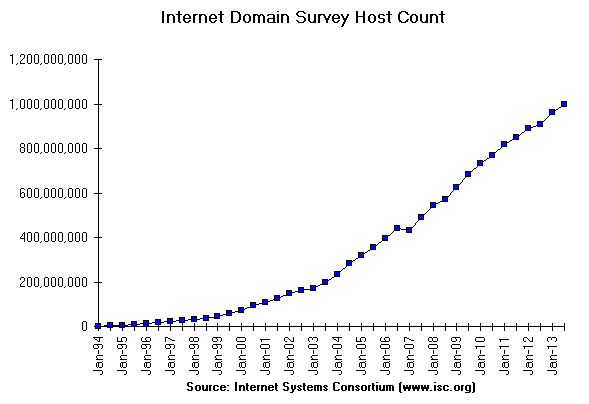
\includegraphics[scale=0.5]{./figures/hosts}
	\caption{L'évolution de nombre d'hôtes sur Interent de $1994$ à $2013$, cette figure  obtenues à partir de site: http://facesncups.com/inforev.html}
	\label{hosts}
\end{figure}
Par conséquent, si nous souhaitons modéliser ces réseaux, on ne peut pas recourir à un modèle statique. Notre approche de modélisation doit plutôt reconnaître que les réseaux sont le produit d'un processus de croissance constant.
\begin{sloppypar}
\subsection{L'attachement préférentielle et le mécanisme "rich get richer"}
\end{sloppypar}
Le modèle de réseau aléatoire suppose que nous choisissons au hasard les partenaires d'interaction d'un nœud. Pourtant, la plupart des réseaux réels de nouveaux nœuds préfèrent se lier aux nœuds les plus connectés, ce processus appelé attachement préférentiel, par exemple. Nous ne connaissons qu'une infime fraction du trillion ou plus de documents disponibles sur le WWW. Les nœuds que nous connaissons ne sont pas entièrement aléatoires: nous avons tous entendu parler de Google et de YouTube, mais nous rencontrons rarement les milliards de nœuds moins importants qui sont dans le Web. Comme nos connaissances sont biaisées vers les documents Web les plus populaires, nous sommes plus susceptibles de lier à un nœud de haut niveau qu'à un nœud avec seulement quelques liens \cite{Barabasi2002}.\\
L'ancienneté, cependant, n'est pas suffisante pour expliquer la loi libre-échelle. Hubs nécessitent l'aide de la deuxième loi, l'attachement préférentiel. Parce que les nouveaux nœuds préfèrent se lier aux nœuds les plus connectés, les premiers nœuds avec plus de liens seront sélectionnés plus souvent et croîtront plus rapidement que les autres qui sont plus jeunes et moins connectés. Comme de plus en plus de nœuds arrivent et continuent de choisir les nœuds les plus connectés, les premiers nœuds vont inévitablement se détacher du paquet, acquérant un très grand nombre de liens. Ils vont se transformer en hubs. Ainsi, l'attachement préférentiel induit un phénomène "rich get richer" qui aide les nœuds les plus connectés à devenir plus connectés. Alors ce phénomène "rich get richer" mène naturellement aux lois libre-échelle observées dans les réseaux réels, on va confirmer cette idée dans la section suivante par notre propre travail et par une façons plus rigueur.
\begin{sloppypar}
\section{Attachement préférentielle sans l'effet "rich get richer"}
\end{sloppypar}
   %\subsection{Introduction}
   \subsection{Le modèle}
À l'instar du modèle BA original, notre réseau évolue selon deux mécanismes: la croissance et l'attachement préférentiel. Les nœuds entrant dans le réseau préfèrent s'attacher à des nœuds de faible degré, alors la probabilité $\Pi(k_i)$ que l'un des liens d'un nouveau nœud se connecte au nœud $i$ dépend de son degré $k_i$ tel que $\Pi(k_i)=C(1-\frac{k_i}{\sum_jk_j})$. où $C$ est la constante de normalisation.\\
En ce qui concerne les réseaux sociaux, si nous considérons le degré de nœuds comme décrivant la richesse des gens dans une société capitaliste, nous savons que nous vivons dans un monde où les riches s'enrichissent, mais quelle sorte de société nous aurons s' il n y a pas de faveur pour les gens riches, et il y a plutôt une subvention continue pour les pauvres ?
   
   Pour mettre en œuvre notre idée, nous commençons par $m_0$ nœuds, chacun avec $m$ liens. À chaque pas de temps, nous ajoutons un nouveau nœud avec $m$ arêtes qui lient le nouveau nœud à $m$ différents nœuds déjà présents dans le réseau. La probabilité que le nouveau nœud soit connecté à un noeud $i$ de degré $k_i$ est $\Pi(k_i)=C(1-\frac{k_i}{\sum_jk_j})$. La constante de normalisation $C$ est déduite de la condition $\sum_{i=1}^{t}\Pi(k_i)=1$, qui donne $C=\frac{1}{t+m_0-1}$. $t$ est le temps à laquelle le dernier nœud a été créé et représente également le nombre de nœuds ajoutés au réseau.
   
   \subsection{Distribution de degrés en utilisant l'équation maîtresse}
   Notons $N(k,t)$ le nombre de nœuds de degré $k$ à l'instant $t$. La distribution de degrés à un instant donné $t$ sera écrit $P(k,t)=\frac{N(k,t)}{N(t)}$. Puisque à chaque pas de temps nous ajoutons un nouveau nœud au réseau, nous avons $N=t$. C'est, à tout moment, le nombre total de nœuds est égal au nombre de pas de temps.\\
   Nous écrivons l'attachement préférentiel dans notre modèle comme
   \begin{equation}
   \Pi(k)=C\big(1-\frac{k}{\sum_jk_j}\big)=C\big(1-\frac{k}{2mt+mm_0}\big)
   \end{equation}
   le terme $2m$ capture le fait que chaque lien contribue au degré de deux nœuds, et $mm_0$ capture le fait que au temps initial nous commençons par $m_0$ nœuds, chacun avec $m$ liens. Notre objectif est de calculer les changements dans le nombre de nœuds de degré $k$ après l'ajout d'un nouveau nœud au réseau. Pour cela, on respecte les deux événements qui modifient $P(k,t)$ suite à l'arrivée d'un nouveau nœud:
   \begin{itemize}
   	\item Un nouveau nœud peut être lié à un nœud de degré $k$, le transformant en un nœud de degré $(k+1)$, ce qui diminue $P(k,t)$.
   	\item Un nouveau nœud peut être lié à un nœud de degré $(k-1)$, le transformant en un nœud de degré $k$, augmentant ainsi $P(k,t)$.
   \end{itemize}
  Alors pour ce modèle, l'équation maîtresse peut être écrite comme suit:
   \begin{equation}
   \begin{aligned}
  (t+1)P(k,t+1)= &tP(k,t)+m\Pi(k-1,t)tP(k-1,t)\\
   & -m\Pi(k,t)tP(k,t)+\delta_{k,m},
  \end{aligned}
 \end{equation}
  où $\delta$ est le symbole Kronecker.\\
  L'équation stationnaire correspondante prend la forme suivante:
  
  \begin{equation}
  \begin{aligned}
  (t+1)P(k)= &tP(k)+m\big(1-\dfrac{k-1}{2mt+mm_0}\big)\dfrac{tP(k-1)}{t-1}\\
  &-m\big(1-\dfrac{k}{2mt+mm_0}\big)\dfrac{tP(k)}{t-1} +\delta_{k,m},
  \end{aligned}
  \end{equation}
pour des temps très grand on peut écrire que $t+1=t$ et $t-1=t$, d'où
 \begin{equation}
 P(k)\big(1+m\big(1-\dfrac{k}{2mt+mm_0}\big)\big)=m\big(1-\dfrac{k-1}{2mt+mm_0}\big)P(k-1) +\delta_{k,m},
 \end{equation}
 après quelque lignes on obtient facilement que:
\begin{align}
P(k)&= 
\begin{cases}
\dfrac{2mt - (k-1)}{2t + 2mt - k}P(k-1), \quad \textrm{for }  k>m,\\
\\
\dfrac{2t}{2t + 2mt - m}, \quad\textrm{for }  k=m.
\end{cases}
\end{align}
La relation de récurrence ci-dessus donne la solution suivante:
\begin{align}
P(k)&= 
\begin{cases}
\dfrac{2t}{2t + 2mt - m}\prod^k_{j=m+1}\left( \dfrac{2mt -j + 1}{2t + 2mt - j}\right), \quad \textrm{for }  k>m,\\
\\
\dfrac{2t}{2t + 2mt - m}, \quad\textrm{for }  k=m.
\end{cases}
\label{eq4-2}
\end{align}
Bien que cette équation ne soit pas fermée, l'estimation numérique de $ P (k) $ est simple comme le montre la figure ~\ref{fig1-2}. \\
Nous simulons également le réseau avec des tailles allant jusqu'à $n=2\times10^6$, le nombre initial des nœuds est $m_0=3$ et $m=2$. 
Les résultats de la simulation supportent fortement les résultats analytiques (voir Fig.~\ref{fig1-2}). 

\begin{figure}[h]
	\centering
	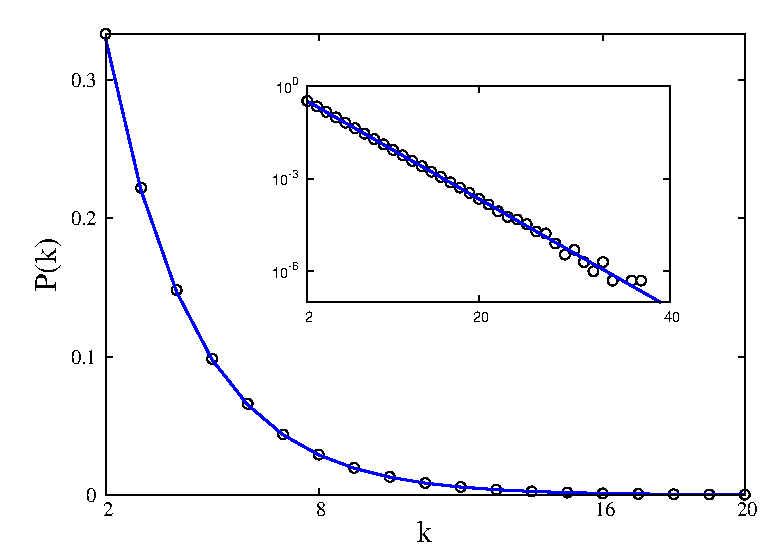
\includegraphics{./figures/fig1}
	\caption{les résultats de simulation (cercles)  pour $n=2.10^6$, $m=2$, $m_0=3$, et la solution numérique (	ligne continue) pour Eq.~\eqref{eq4-2}. Dans l'insérer, nous tracerons les mêmes données dans l'échelle log-linéaire.}
	\label{fig1-2}
 \end{figure} 
Nous avons observé dans les simulations que $k$ reste inférieur à $40$ pour $t=2.10^6$, nous prenons alors $t\gg j $ dans Eq.~\ref{eq4-2} et nous obtenons
\begin{align}
P(k)&\approx 
\begin{cases}
\dfrac{1}{1+m}\Big(\dfrac{m}{1+m}\Big)^{k-m-1}, \quad \textrm{for }  k>m,\\
\\
\dfrac{1}{1+m}, \quad\textrm{for }  k=m.
\end{cases}
\label{eq5-2}
\end{align}
Après la normalisation, nous obtenons la distribution des degrés exponentielle $P(k)=Ae^{-A(k-m)}$, avec $A=\log(\dfrac{m+1}{m})$.
L'insérer de la figure Fig.~\ref{fig1-2} montre la forme exponentielle de $ P(k)$ et l'excellent accord entre les simulations et les résultats théoriques.
Ceci confirme clairement que l'attachement préférentiel seul n'est pas suffisant pour produire des réseaux libre-échelle.

\subsection{Comparaison au niveau microscopique avec le modèle de BA}
 Nous recherchons les différences entre réseaux hétérogènes et homogènes en comparant notre modèle au modèle BA. La distribution des degrés ne suffit pas à elle seule à caractériser les réseaux. Le calcul d'autres quantités microscopiques peut aider à mieux comprendre leur évolution et leur formation. Il s'avère que le réseau libre-échelle a des nœuds avec un degré important (hubs), tandis que le réseau aléatoire n'a pas de structure apparente. L'évaluation du degré moyen instantané du nœud cible $\kms$ et de ses fluctuations peut fournir des informations quantitatives sur les nœuds du réseau. En fait, $\kms$ est en quelque sorte lié au degré moyen instantané des hubs, car lors du choix aléatoire des nœuds, les hubs ont plus de chance d'être sélectionnés. \\  
 Dans un premier temps, nous analysons $\kms$ et $\kmss$ dans le réseau BA
 \begin{eqnarray}
 \kms=\sum_{t_i=1}^t\Pi(k_i)k_i(t)+m_0\Pi(k_0)k_0(t),
 \label{eq6-2}
 \end{eqnarray}
 où  $\Pi(k_i)=\frac{k_i(t)}{2mt+mm_0}$, $t_i$ est le temps à laquelle le nœud $ i $ a été créé et $ k_0 (t) $ est le degré des nœuds initiaux à l'instant $t$.\\
 $k_i (t)$ est facilement calculé à partir de l'équation d'évolution du degré de champ moyen:
 $\dfrac{\partial k_i(t)}{\partial t}=~ m\Pi(k_i)$, qui donne $k_i(t)=m\Big(\frac{2t+m_0}{2t_i+m_0}\Big)^{\frac{1}{2}}$.\\
 En insérant la dernière expression dans l'Eq.~\ref{eq6-2}, on obtient
 \begin{eqnarray}
 \kms&=&m\Big(\sum_{t_i=1}^{t}\dfrac{1}{2t_i+m_0}+1\Big) \\
 &=&m \Big(\ln (2t+m_0)+\gamma-a+\frac{1}{2(2t+m_0)}+O(\frac{1}{t^2})\Big),
 \label{eq7-2}
 \end{eqnarray}
 où $\gamma$ est la constante d'Euler, et $a=\frac{1}{2}+\frac{1}{3}+\ldots+\frac{1}{1+m_0}$.\\
 Un bon accord est obtenu comme le montre la figure Fig.~\ref{fig2a-2} entre Eq.~\ref{eq7-2} et les résultats de la simulation même pour les premiers instants de l'évolution. $\kms$ croît indéfiniment avec le temps et diverge pour un réseau infini (oo $t\to\infty$) du fait que, dans les réseaux hétérogènes, les hubs sont plus susceptibles d'être sélectionnés et liés à de nouveaux nœuds. \\
 De l'autre côté, le degré moyen du réseau reste fini \cite{Barrat-a2008l,Cohen-Havlinl2010} puisque la majorité des nœuds ont un faible degré et le poids des hubs est faible.\\
 \begin{figure}[h]
 	\centering
  	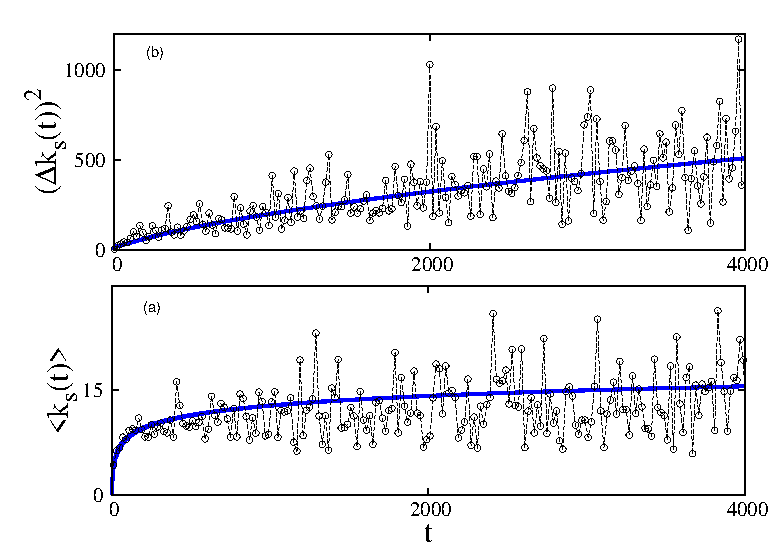
\includegraphics[scale=0.85]{./figures/nfig2}
 	\caption{(a) Évolution de $\kms$ dans le modèle BA, la ligne continue représente Eq.~\ref{eq7-2}.
 	(b) Évolution des fluctuations de $\kms$, la ligne continue représente Eq.~\ref{eq10-2}. Les cercles joints par des lignes pointillées dans les deux cas sont des données de simulation moyennées sur 20 réalisations pour $m =2$, $m_0=3$.}
 	\label{fig2a-2}
 \end{figure}
 
 Le deuxième moment $\kmss$ s'écrit
 \begin{align}
 \kmss&=\sum_{t_i=1}^t\Pi(k_i)k^2_i(t)+m_0\Pi(k_0)k_0^2(t)\label{eq8-2} \\
 &\approx m^2(2t+m_0)^{\frac{1}{2}} \Big(\sum_{t_i=1}^t \frac{1}{(2t_i+m_0)^{\frac{3}{2}}}+m_0^{-\frac{1}{2}}\Big).
 \end{align}
 Pour des grands temps, $\sum_{t_i=1}^t\Big(\frac{1}{t_i}\Big)^{\frac{3}{2}}=\zeta(\frac{3}{2}) \approx 2.612$, on obtient 
 \begin{eqnarray}
 \begin{split}
 \kmss&\approx m^2\sqrt{2t}(m_0^{-\frac{1}{2}}+2.612-b),
 \label{eq9-2}
 \end{split}
 \end{eqnarray}
où $b=1+\frac{1}{2^\frac{3}{2}}+\frac{1}{3^\frac{3}{2}}+\ldots+\frac{1}{(1+m_0)^\frac{3}{2}}$.\\
Fluctuations de $\kms$ sont donnés par
\begin{align}
(\Delta k_s(t))^2 \equiv \kmss-\kms^2\approx m^2 \Big[(m_0^{-\frac{1}{2}}+2.612-b)\sqrt{2t}-(\ln(2t))^2\Big],
\label{eq10-2}
\end{align}
qui deviennent arbitrairement large lorsque le temps augmente suffisamment. \\
Les données de simulation selon Eq.~\ref{eq10-2} ( voir Fig.~\ref{fig2a-2}(b)) montrent la tendance croissante des fluctuations de $\kms$.
Cela peut s'expliquer par le fait que le degré maximum dans le réseau $k_{max}\sim \sqrt{t}$ \cite{Cohen-Havlinl2010} augmente plus vite que $\kms\sim \ln(t)$ (Eq.~\ref{eq7-2}) et la différence entre les deux quantités devient plus grande avec le temps. \\
Nous passons maintenant à la même analyse dans notre modèle,  L'équation d'évolution du champ moyen pour $k_i(t)$ est donnée par
\begin{eqnarray}
\dfrac{\partial k_i(t)}{\partial t}=m\Big(1-\dfrac{k_i(t)}{2mt+mm_0}\Big)\dfrac{1}{t+m_0-1},
\end{eqnarray}
La solution a la forme
\begin{eqnarray}
k_i(t)=m \Big(\frac{t+m_0-1}{2t+m_0}\Big)^{\frac{1}{m_0-2}}\Bigg[\Big(\frac{t_i+m_0-1}{2t_i+m_0}\Big)^{-\frac{1}{m_0-2}}-A(t_i)
+A(t)\Bigg],
\label{kit}
\end{eqnarray}
où $A(t)=\displaystyle \int_1^{t}\dfrac{\Big(\frac{t'+m_0-1}{2t'+m_0}\Big)^{-\frac{1}{m_0-2}}}{t'+m_0-1}dt'$.\\
On sait que la valeur moyenne du nœud sélectionné $\kms$ est sous la forme 
\begin{eqnarray}
\kms=\sum_{t_i=1}^t\Pi(k_i)k_i(t)+m_0\Pi(k_0)k_0(t),
\label{kms-2}
\end{eqnarray}
 en remplaçant Eq.~\ref{kit} dans cette dernière équation on obtenue immédiatement pour tout temps $ t $ l'expression de $\kms$, L'équation résultante est résolue numériquement comme le montre Fig.~\ref{fig2b-2}. \\
Pour large temps et en prenant $t \gg m_0$, nous trouvons 
$A(t)\approx 2^{\frac{1}{m_0-2}} \ln(t)$, $k_i(t)\approx m\Big(1+\ln \dfrac{t}{t_i}\Big)$, d'où
\begin{align}
\label{kom}
\kms&\approx\dfrac{m}{t}\Big(\sum_{t_i=1}^{t} \ln(t)-\ln(t_i)+1\Big)\\
&\approx\dfrac{m}{t}\Big(t \Big(\ln(t)+1\Big)-\Big(\sum_{t_i=1}^{t} \ln(t_i)\Big)\Big) \nonumber \\
&\approx\dfrac{m}{t}\Big(t\ \Big(\ln(t)+1\Big)-\ln(t_i!)\Big) \nonumber \\
&\approx2m. \nonumber
\end{align}

Le second moment est obtenu en substituant les expressions correspondantes de $\Pi(k_i)$ et $k_i(t)$ dans Eq.~\ref {eq8-2}, nous obtenons pour de large temps
 \begin{eqnarray}
\begin{split}
\kmss\approx \frac{m^2}{t}\Big(\sum_{t_i=1}^t (\ln(\frac{t}{t_i})+1)^2\Big).
\label{k2om}
\end{split}
\end{eqnarray}
Faire les approximations  $\sum_{t_i=1}^t \ln(t_i)\approx t\ln(t)-t$, et
$\sum_{t_i=1}^t \ln(t_i)^2\approx t\ln(t)^2-2t\ln(t)+2t-2$, on obtient $\kmss\approx 5m^2.$ Fluctuations sont 
\begin{eqnarray}
 (\Delta k_s(t))^2 \equiv {\kmss-\kms^2}\approx m^2.
\end{eqnarray}
 Cette résultat, ensemble avec $\kms\approx 2m $, montrent que presque tous les nœuds ont le même degré que celui illustré sur Fig.~\ref{fig2b-2}. L'homogénéité du réseau peut s'expliquer par le fait que l'attachement préférentiel utilisé ici ne permet pas la formation de hubs, puisqu'il ne permet pas aux riches de s'enrichir, ni d'enrichir les pauvres. 
\begin{figure}[h]
	\centering
	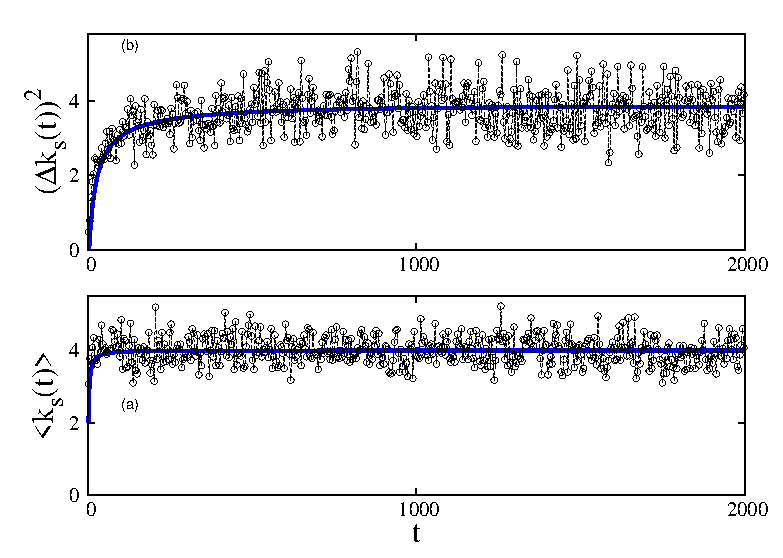
\includegraphics[scale=1]{./figures/nfig3}
	\caption{(a) Évolution de $\kms$ dans notre modèle, la ligne continue représente Eq.~\ref{kms-2}.
	(b) Évolution des fluctuations de $\kms$, la ligne continue représente la solution numérique de Eq.~\ref{kms-2} et Eq.~\ref{k2om}. Les cercles joints par des lignes pointillées dans les deux cas sont des données de simulation moyennées sur $20$ réalisations pour $m=2$, $m_0=3$.}
	\label{fig2b-2}
\end{figure}
 \vspace{4cm}
\section{conclusion}

Dans ce chapitre, nous avons commencé de donner quelques idées sur les processus dynamiques, l'attachement préférentielle et le mécanisme "rich get richer" dans les réseaux réels , puis nous avons introduit un simple modèle de réseau complexe avec un critère d'attachement préférentiel et sans effet "rich get richer". Le réseau obtenu est homogène, ce qui démontre le rôle crucial du "rich get richer" dans la topologie du réseau, en outre on a conclu que le fait de donner un traitement préférentiel aux nœuds les moins connectés équivaut à utiliser une probabilité d'attachement aléatoire. \\
Le Calcul du degré moyen instantané d'un nœud sélectionné et ses fluctuations fournissent plus d'informations que le degré moyen habituel du réseau, en particulier nous avons montré comment le degré moyen de hubs et ses fluctuations divergent avec le temps dans le modèle BA, et restent finis dans notre modèle.
%En termes de répartition de la richesse sociale, le principe de Pareto \cite{Pareto1897} ne s'applique pas et nous avons plutôt une distribution exponentielle du revenu.
%\newcommand{\nl}{$n_{\ell}$ }
\newcommand{\km}{\textless k \textgreater}
\chapter{Structure des réseaux sans échelle non corrélés: couches et plus court chemin}
\label{sec3}
\begin{minipage}{\textwidth}
	\linespread{1.2}
	\minitoc
\end{minipage}

\section{Introduction}
L'objectif principal de ce chapitre vise à prédire la structure des couches
des réseaux sans échelles en nous basant sur les propriétés locales régissant les sommets individuels.\\
De nombreux réseaux du monde réel qui ont été décrits précédemment, tels que le WWW et les réseaux de collaboration, grandissent avec le temps. Par conséquent, il est raisonnable de considérer les graphes de taille croissante et d'étudier la structure de ces réseaux ayant souvent la propriété sans échelle (voir Section.\ref{s-libre-echelle}). 
La communauté scientifique, en s'appuyant sur des idées issues d'une grande variété de disciplines, a fait un excellent départ sur la caractérisation et la modélisation de la structure des réseaux, mais il n'y pas encore de formalisme théorique bien établi \cite{Ne2003}. Dans ce chapitre nous allons expliquer notre contribution à la compréhension de la structure intrinsèque des réseaux sans échelle. En particulier, nous allons calculer le nombre moyen de voisins d'un nœud  donné se trouvant à une distance précise, et nous allons en déduire le plus court chemin dans le réseau.% Nous allons commencer par quelques propriétés et définitions, et ensuite on va rappeler quelques travaux importants dans le sujet. Dans la dernière section du chapitre nous exposons nos calculs  détaillés.
\section{Caractérisation des réseaux sans échelle}
Un réseau sans échelle (ou réseau invariant d'échelle, ou encore scale-free network en anglais) est un réseau dont la distribution des degrés suit une loi de puissance, c'est-à-dire, $P(k)=Ck^{-\gamma}$, où $C$ est une constante.  Donc, dans un tel réseau, la proportion de nœuds de degré $k$ est proportionnelle à $k^{-\gamma}$. Cette loi traduit l'absence d'échelle caractéristique. En effet, si on multiplie $k$ par une constance $\alpha$, $P(\alpha k)=C\alpha^{-\gamma}k^{-\gamma}=C' k^{-\gamma}$, donc les propriétés sont les mêmes si on change l'échelle.\\ 
Identifier la loi de puissance dans les systèmes naturels ou artificiels peut être difficile. La stratégie standard utilise le fait que la courbe d'une distribution sans échelle apparaît comme une ligne droite lorsqu'elle est tracée sur des échelles logarithmiques (voir Fig.~\ref{sans-echelle-3}).
\begin{figure}[h!]
	\centering
	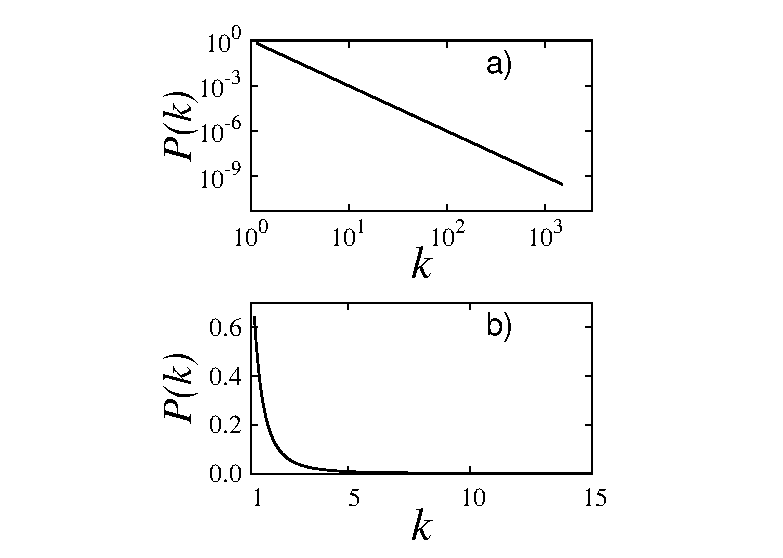
\includegraphics[scale=1.2]{./figures/fig-sans-echelle}
	\caption{Illustration de la loi de puissance pour une fonction, $P(k)=k^{-\gamma}$, avec l'exposant $\gamma=3$. Dans a) l'échelle est logarithmique et dans b) l'échelle est linéaire.}
	\label{sans-echelle-3}
\end{figure}
Cependant, la méthode n'est pas très bonne à certains égards. En particulier, l'extrémité de la droite de la distribution est bruyante en raison d'erreurs d'échantillonnage (voir Fig.~\ref{BA-distribution}). Du fait que la distribution diminue dans l'extrémité,  chaque valeur mesurée ne contient que quelques échantillons, et les fluctuations dans les valeurs mesurées sont grandes, et cela apparaît comme une courbe bruyante sur la figure. Une façon de traiter cela est de simplement jeter les données dans la queue de la courbe. Mais il y a souvent des informations utiles dans ces données, car de nombreuses distributions suivent une loi de puissance seulement dans la queue. Une solution alternative consiste à faire varier la largeur des cases dans notre courbe. Le nombre d'échantillons dans une largeur $\Delta x$ devrait être divisé par $\Delta x$ pour obtenir une moyenne par intervalle unitaire de $x$. Ensuite, le nombre d'échantillons normalisé devient indépendant de la largeur de la valeur mesurée en moyenne, et nous sommes libres de varier les largeurs $\Delta x$ comme nous le souhaitons. Le choix le plus commun est de créer des largeurs telles que chacune est un multiple fixe plus large que celui qui le précède, ce qui est connu sous le nom "logarithmic binning". Ceci réduit les erreurs statistiques dans la queue. En outre, les valeurs mesurées semblent être de largeur constante quand nous traçons la courbe sur des échelles logarithmiques.
\section{Quelques notions mathématiques de la loi de puissance}
Une variable réelle continue avec une distribution en loi de puissance a une probabilité $P(k)$ de prendre une valeur $k$, où
\begin{equation}
P(k)=Ck^{-\gamma}.
\label{3-1}
\end{equation}
Comme nous avons vu dans la Section.~\ref{s-libre-echelle}, l'exposant $\gamma$ et la variable $k$ sont positifs. \\
Dans les réseaux réels, les distributions de degrés ne suivent généralement pas une loi de puissance pure sur toute leur gamme.
En regardant la Fig.~\ref{scal-free-reels}, par exemple, nous observons que la distribution de degrés n'est pas toujours monotone pour les petits $k$, même en tenant compte des fluctuations statistiques dans l'histogramme. Quand on dit qu'un réseau a une distribution de degré sans échelle, on se réfère implicitement à la queue de la distribution, qui doit avoir cette forme. Cependant, et dans certains cas, la distribution peut  s'écarter de la loi d'échelle pour $k$ élevé. En fait, il y a parfois une coupure qui limite le degré maximum de nœuds dans la queue.\\
La constante $C$ dans l'Eq.~\eqref{3-1} est la constante de normalisation qui s'obtient en intégrant:
\begin{equation}
P(k)=\int_m^{\infty}Ck^{-\gamma}dk=1,
\label{3-2}
\end{equation}
où $m$ est le degré minimum dans le réseau, on obtient
\begin{equation}
C=(\gamma-1)m^{\gamma-1},
\end{equation}
alors l'Eq.~\eqref{3-1} devient:
\begin{equation}
P(k)=(\gamma-1)m^{\gamma-1}k^{-\gamma}.
\label{3-4}
\end{equation}
%\subsection{Moments}
Le $j^{\text{ème}}$ moment de la distribution $P(k)$ est défini comme:
\begin{align}
\textless k^j\textgreater&=\int_{m}^{\infty} k^jP(k)dk\nonumber\\
&=(\gamma-1)m^{\gamma-1}\int_{m}^{\infty}k^{j-\gamma}dk.
\end{align}
Le premier moment $\textless k\textgreater$  est le degré moyen de $k$, notons que $\textless k\textgreater$  devient infini si $\gamma\leq2$. Le second moment $\textless k^2\textgreater$ mesure les fluctuations de $k$, il diverge si $\gamma\leq3$. Sachant que dans les réseaux réels l'exposant $\gamma$ est souvent dans l'intervalle $2<\gamma<3$, ceci implique que les fluctuations divergent dans ces réseaux.\\
%\subsection{Loi sans échelle pour les variables discrètes
En réalité, dans un réseau, les degrés sont des entiers naturels, et dans nos calculs les intégrales doivent être remplacées par des sommes. Mais, puisque la loi d'échelle
n'est vérifiée que pour les grands degrés, ceux-ci peuvent être considérés comme représentant  une variable continue.\\
Techniquement, si $k$ est une variable discrète, et $P(k)=Ck^{-\gamma}$, alors la constante de normalisation $C$ doit vérifier $\sum_{k=1}^{\infty}Ck^{-\gamma}=1$, donc $C=\frac{1}{\zeta(\gamma)}$, et $\zeta(\gamma)$ est la fonction zêta de Riemann. Donc la loi de puissance, si $k$ est discret, s'écrit:
\begin{equation}
P(k)=\frac{1}{\zeta(\gamma)}k^{-\gamma}.
\label{pk-descret}
\end{equation}
Dans les calculs on a souvent besoin de connaître la valeur du degré maximum $K$, mais dans un réseau dans échelle en croissance, ce n'est pas possible de connaître sa valeur exacte. Pour estimer la valeur de $K$, on suppose que dans un réseau fini avec $n$ nœud , on peut avoir au plus un nœud dans l'intervalle $[K,\infty[$, c'est-à-dire, la probabilité d'observer un nœud avec un degré supérieur à $K$ est $\frac{1}{n}$, donc:
\begin{equation}
\int_{K}^{\infty}P(k)dk=\frac{1}{n},
\end{equation}
d'où on obtient $K= mn^{\frac{1}{\gamma-1}}$.
\section{Les réseaux sans échelle non corrélés}
Dans les modèles aléatoires sans échelle, on suppose généralement qu'il n'y a pas de corrélation entre les degrés des nœuds voisins. C'est-à-dire que la probabilité d'atteindre un nœud en suivant un lien est indépendante du nœud d'où provient le lien. Cependant, dans de nombreux réseaux du monde réel, ce n'est pas le cas. Plusieurs types de corrélations existent en fonction des propriétés des nœuds. Les principaux types de corrélations étudiées sont les corrélations degré-degré (voir Section.\ref{s-correl}). Même si la construction de ces réseaux sans échelle aléatoires se fait au départ sans aucune corrélation, cela ne signifie pas que le réseau n'affichera pas des corrélations de degré, c'est-à-dire l'absence de corrélations lors de la création des réseaux n'entraîne pas l'absence de corrélations dans le réseau formé.  La Fig.~\ref{correlation} indique que les réseaux aléatoires sans échelle présentent des corrélations de degré, allant de l'assortativité à la dissassortativité selon la valeur de l'exposant $\gamma$. Nous observons trois situations:
%\begin{spacing}{1.5}
\begin{itemize}
	\item[i)] $\gamma>3$, le réseau est dit assortatif. Dans ce cas, la corrélation entre les degrés des sommets et ceux de leurs voisins est élevée. Autrement dit, les sommets ayant un degré élevé sont connectés entre eux; les sommets ayant un degré faible sont connectés entre eux et il y a peu de liens entre les sommets de degré élevé et ceux de degré faible 
	\item[ii)]$\gamma=3$, le réseau est neutre.
	\item[iii)]$\gamma<3$, le réseau est dissassortatif. C'est le cas contraire à l'assortativité. Les sommets voisins sont peu corrélés, et les sommets avec un degré élevé sont connectés à ceux avec un degré faible.  
\end{itemize}
%\end{spacing}
Générer des corrélations en utilisant un modèle complètement statique est difficile car non seulement le degré d'un nœud doit être pris en compte, mais aussi sa probabilité de se connecter à chaque voisin. La méthode habituellement utilisée pour générer ces réseaux corrélés consiste à mélanger les liens en utilisant une sorte d'algorithme de type Metropolis\footnote{Inventé en 1953 par Nicholas Metropolis et ses collaborateurs du laboratoire de Los Alamos, l'algorithme de Metropolis était d'abord destiné à faire calculer par des ordinateurs les équations d'états de mélanges de molécules en interactions. L'outil principal de l'algorithme est une chaîne de Markov : on tire au hasard une boule et on déplace son centre d'une distance $d$, le mouvement est accepté si la nouvelle configuration des boules reste sans recouvrement.} \cite{Metropolis-al1953}.\\ Cependant, la négligence de ces corrélations n'empêche jamais de trouver des résultats importants, qui nous aideront à bien modéliser ces réseaux réels et à mieux comprendre leurs structures. 
\begin{figure}[h!]
	\centering
	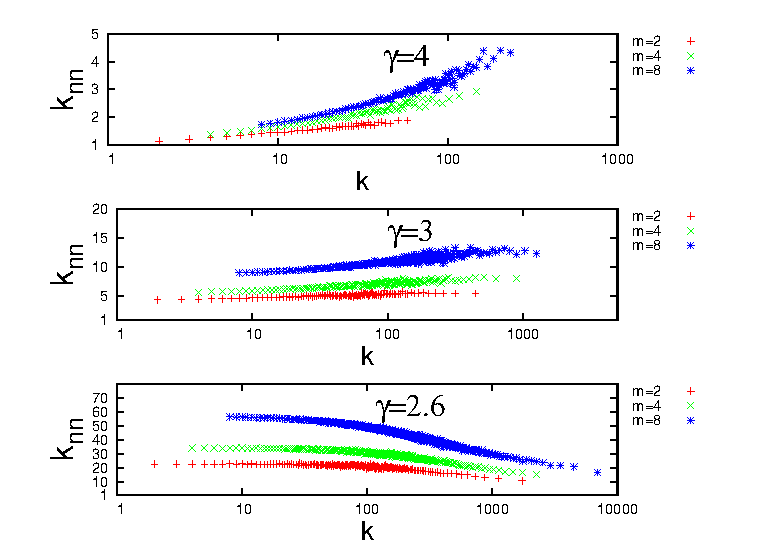
\includegraphics[scale=1.2]{./figures/correlation}
	\caption{Les corrélations des degrés dans le réseau aléatoire sans échelle pour différents valeurs de $m$ et de $\gamma$. Le nombre de nœuds est $n=10^4$ et le nombre de réalisations pour chaque simulation est $50$.}
	\label{correlation}
\end{figure}
\vspace{3cm}
\section{Structure des couches dans les réseaux sans échelle non corrélés}
\subsection{Quelques contributions importantes}
Newman est l'un des premiers à chercher une expression explicite pour les couches dans les réseaux complexes \cite{Newman2010-456}, où le mot couche désigne le nombre moyen de nœuds à une distance donnée d'un nœud arbitraire choisi au hasard, et qu'on appelle nœud racine.\\
Le calcul de Newman se base sur la fonction génératrice qui suscite un intérêt particulier dans les réseaux complexes. En effet, celle-ci donne toute l'information sur la distribution des degrés $P(k)$. La fonction génératrice est le polynôme:
\begin{equation}
g(z)=P(0)+P(1)z+P(2)z^2+...=\sum_{k=0}^{\infty}P(k)z^k.
\end{equation}
Si on connaît la fonction génératrice, on peut récupérer les valeurs de $P(k)$ en différenciant:
\begin{equation}
P(k)=\frac{1}{k!}\frac{d^kg(z)}{dz^k}\Big\lvert_{z=0}.
\end{equation}
Ainsi, la distribution de probabilité et la fonction génératrice ne sont en réalité que deux représentations différentes de la même chose. Dans de nombreux cas, il est plus facile de travailler avec la fonction génératrice qu'avec la distribution de probabilité.\\
Soit $p_k^{(2)}$ la probabilité qu'un nœud a exactement $k$ seconds voisins dans le réseau
\begin{equation}
p_k^{(2)}=\sum_{s=0}^{\infty}P(s)P^{(2)}(k/s),
\end{equation}
avec $P^{(2)}(k/s)$ la probabilité d'avoir $k$ seconds voisins étant donné que nous avons $s$ premiers voisins, et $P(s)$ est la distribution de degrés.\\
La fonction génératrice de cette probabilité s'écrit:

\begin{align}
	g^{(2)}(z)&=\sum_{k=0}^{\infty}p_k^{(2)}z^{k}\nonumber\\
	%&=\sum_{m=0}^{\infty}p_m\sum_{k=0}^{\infty}P^{(2)}(k/m)z^k\nonumber\\
	%&=\sum_{m=0}^{\infty}p_m[g_1(z)]^m\nonumber\\
	&=g_0(g_1(z)),
	\label{p-generatrice-2}
\end{align}
avec $g_0(z)=\sum_{k=0}^{\infty}P(k)z^k$ et $g_1(z)=\frac{1}{g'_0(1)}\frac{dg_0}{dz}$, (nous utiliserons la notation $g'$, car elle s'avère beaucoup moins lourde que la notation plus courante $\frac{dg}{dz}$.).\\
En généralisant la procédure, Newman a trouvé la fonction génératrice du nombre de voisins à n'importe quelle distance $\ell$, qui s'écrit:
\begin{align}
g^{(\ell)}(z)&=\sum_{s=0}^{\infty}p_s^{(\ell-1)}\sum_{k=0}^{\infty}P^{(\ell)}(k/s)z^k\\
&=g^{(\ell-1)}(g_1(z)),
\label{p-generatrice-l}
\end{align}
avec $g^{(\ell)}(z)=g_0(...g_1(z)...)$, où dans $g_0$ il y a $\ell-1$ copie de $g_1$.\\
Il est généralement difficile d'extraire les expressions explicites des probabilités à partir de l'équation précédente, et ce m\^{e}me pour le cas des seconds voisins. Cependant, pour une distribution de degrés suivant la loi de Poisson avec une moyenne $\km$, $P(k)=\frac{\km^k}{k!}e^{-\km}$, et si on suppose que $z=1$, le calcul se simplifie pour le nombre de seconds voisins, et on trouve:
\begin{equation}
n_2=g_0'(1)g_1'(1),
\label{3-27}
\end{equation}
sachant que $g_0'(1)=\km$ et $g_1'(1)=\frac{1}{\km}(\textless k^2\textgreater-\km)$, on obtient
\begin{equation}
n_2=\textless k^2\textgreater-\km.
\end{equation}
Le nombre moyen de voisins $n_{\ell}$ à n'importe quelle distance $\ell$, pour une distribution de poisson, est obtenu à partir de l'Eq.~\eqref{p-generatrice-l}:
\begin{equation}
\frac{dg^{(\ell)}}{dz}=g^{(\ell-1)'}(g_1(z))g_1'(z),
\end{equation}
sachant que nous avons choisi $z=1$ nous pouvons écrire 
\begin{align}
n_{\ell}&=g^{(\ell-1)'}(1)g_1'(1)\\
&=n_{\ell-1}g_1'(1),\nonumber
\end{align}
de l'Eq.~\eqref{3-27}, et sachant que $g_0'(1)=\km=n_1$ et que $g_1'(1)=\frac{n_2}{n_1}$, on obtient: 
\begin{equation}
n_{\ell}=n_{\ell-1}\Big(\frac{n_2}{n_1}\Big),
\end{equation}
nous pouvons écrire finalement que la distribution des nœuds voisins à une distance $\ell$ d'un nœud choisi au hasard est:
\begin{equation}
 n_{\ell}=\Big(\frac{n_2}{n_1}\Big)^{\ell-1}n_1.
\end{equation} 
Cela signifie que \nl augmente ou diminue exponentiellement avec $\ell$ selon que $n_2$ est supérieur ou inférieur à $n_1$.\\
La solution de Newman pour la $\ell^{\grave eme}$ couche est une fonction monotone, c'est-à-dire soit croissante soit décroissante, ce qui est loin du comportement des réseaux réels \cite{Cohen-Havlinl2010}.

Une autre contribution importante dans le sujet est celle de Cohen et al. \cite{Cohen-Havlinl2010-72,Kalisky-al2006}. Le calcul dans ce cas est basé sur le travail de Bollobás \cite{Bollobas1985}. On commence par attribuer à chaque nœud un degré, et donc des liens disponibles. Le réseau est ensuite construit en commençant par connecter le nœud de degré maximum $K$ aléatoirement avec $K$ liens du réseau, ce qui constitue les nœuds de la première couche. Dans la deuxième étape, les liens disponibles de la première couche se connecte avec d'autres liens disponibles d'une façon aléatoire, remplissant ainsi la deuxième couche. Cette procédure continue jusqu'à ce qu'il n' y ait plus de liens disponibles.\\
Le traitement analytique de Cohen et al. n'aboutit pas à une expression explicite sous forme d'équation fermée. Leur résultat est donné sous forme d'une équation de récurrence qui se compare bien avec le réseau Internet dans le cas particulier où le degré minimum dans le réseau est $1$.\\
Autres auteurs ont utilisés l'approche de la cavité pour déduire des équations de récurrence pour le nombre moyen de nœuds se trouvant à une distance donnée d'un nœud arbitraire \cite{Nitzan2016}. Dans ce cas, le réseau étudié est le modèle de configuration\footnote{Le modèle de configuration est une méthode pour générer des réseaux aléatoires à partir d'une séquence des degrés de nœuds qui sont préalablement fixés.}.\\
Plus récemment, des résultats analytiques pour le réseau d'Erd\"os-R{\'e}nyi ont été développé dans le régime sous-critique \cite{Katzav-al2015, Katzav-al2018}.
\subsection{Nouvelle approche}
Notre calcul est basé sur le fait que pour les grands réseaux non corrélés, la structure arborescente est vérifiée, et les cycles dans une même couche sont absents \cite{Cohen-Havlin2003,Cohen-Havlin2009}. Par la suite, la probabilité $ p_{\ell} $ qu'un nœud de la couche $n_\ell$ soit lié à un autre nœud n'appartenant pas aux premières $\ell$ couches est $p_{\ell}=\frac{\kappa_{\ell}-1}{n}$, où $\kappa_{\ell}$ est le degré moyen des nœuds appartenant à la couche $\ell$, et le $-1$ est dû au lien de la couche précédente. \\
La probabilité qu'un nœud parmi les $n-n_1-1$ ne soit lié à aucun nœud dans la couche $\ell=1$ est $(1-p_1)^{n_1}$, alors la probabilité que ce nœud soit lié à la couche $\ell=1$ est $1-(1-p_1)^{n_1}$. Le nombre de nœuds dans $\ell=2$ est alors donné par $n_2=(1- (1-p_1)^{n_1})(n-n_1-1)$. La généralisation pour la couche $\ell$ est simple, on obtient:
\begin{align}
n_{\ell}= (1-(1-p_{\ell-1})^{n_{\ell-1}})(n-\sum_{j=1}^{\ell-1} n_j-1).
\label{eq1}
\end{align}
Lorsque $n$ est grand $p_{\ell}\ll1 \Longrightarrow (1-p_{\ell-1})^{n_{\ell-1}}\simeq e^{-p_{\ell-1}n_{\ell-1}} $. L'Eq.~\eqref{eq1} peut être facilement manipulée pour obtenir:
\begin{align}
n_{\ell} &=
\begin{cases}
\km & \text{si}\qquad \ell=1 \\
(n-1-n_1)(e^{-\sum_{j=1}^{\ell-2}p_j n_j}-e^{-\sum_{j=1}^{\ell-1}p_j n_j}) & \text{si}\qquad \ell \ge 2.
\end{cases}
\label{eq2}
\end{align}
L'équation ci-dessus peut être simplifiée en développant les sommes dans les exponentielles. $p_{\ell}$ dépend de $\kappa_{\ell}$, qui dépend à son tour de $\gamma$ et du degré maximum dans la couche $\ell$, $K_{\ell}$.\\
$\kappa_{\ell}$ est facilement calculée, quand $K_{\ell}\gg m$ on trouve:
\begin{align}
\kappa_{\ell} =\frac{<k_{\ell}^2>}{\textless k_{\ell} \textgreater}=&
\begin{cases}
\Big(\frac{\gamma-2}{\gamma-3}\Big)m & \text{si} \qquad \gamma >3 \\ 
m (\ln(K_{\ell})-\ln(m))  & \text{si} \qquad \gamma =3 \\
\Big(\frac{\gamma-2}{3-\gamma}\Big)m^{\gamma-2} K_{\ell}^{3-\gamma}  & \text{si} \qquad 2<\gamma<3 \\
\frac{K_{\ell}-m}{\ln(K_{\ell})-\ln(m)} & \text{si} \qquad \gamma=2.
\end{cases}
\label{eq4}
\end{align}
Lorsque $\gamma=2$, le degré maximum dans le réseau $K$ est de l'ordre du nombre total de nœuds, c'est-à-dire  presque tous les nœuds sont connectés au nœud de degré maximum. Le réseau peut contenir un maximum de deux couches, avec $n_1=\km$ et $n_2=n-\km $. \\
Quand $2\textless \gamma \textless 3$, le réseau est très hétérogène. $\kappa_{\ell} $ dépend de la couche $\ell$ à travers le degré maximum $K_{\ell}$(Eq.~\eqref{eq4}). L'étape suivante de nos calculs consiste à relier $\kappa_{\ell}$ à $\kappa_1$ via $K_{\ell}$. Pour réaliser cette tâche non triviale, nous remplaçons le réseau sans échelle ordinaire par un réseau hypothétique sans échelle et ordonné (Fig.~\ref{fig1}). Nous commençons par choisir aléatoirement un nœud, appelé racine, ayant un degré moyen $\km$. Ses  voisins premiers, seconds, tiers, \ldots, sont placés respectivement dans les couches $\ell=1$, 2, 3, \ldots, allant progressivement et dans l'ordre décroissant, du nœud ayant le plus grand degré dans la première couche au nœud avec le plus petit degré dans la dernière couche. Le nombre de nœuds dans chaque couche est la somme des degrés des nœuds de la couche précédente. Par construction, la première couche contiendra $\km$ nœuds, donc $n_1=\km$.\\
L'idée sous-jacente à cette construction est que pour $\gamma \in ]2,3[$ , les réseaux sans échelle  sont dissassortatives, donc les nœuds sont plus probablement liés aux hubs.\\
\begin{figure}[h]
	\centering
	\begin{tikzpicture}[scale=0.35]
	\tikzstyle{lien}=[-,thick,circle]
	\tikzset{individu/.style={draw,circle,scale=2,fill=black},individu/.default={green},scale=0.7}
	\node[individu,scale=0.3] (a0) at (-1,0) {};
	\node[individu,scale=0.6] (a1) at (2.5,-8) {};
	\node[individu,scale=0.52] (a2) at (-1,-9.18) {};
	\node[individu,scale=0.46] (a3) at (-4.5,-8) {};
	\node[individu,scale=0.44] (b1) at (5,-15.5) {};
	\node[individu,scale=0.42] (b2) at (3,-16.55) {};
	\node[individu,scale=0.4] (b3) at (1.,-17.25) {};
	\node[individu,scale=0.38] (b4) at (-1,-17.6) {};
	\node[individu,scale=0.36] (b5) at (-3.,-17.45) {};
	\node[individu,scale=0.34] (b6) at (-5,-16.92) {};
	\node[individu,scale=0.32] (b7) at (-7,-16.1) {};
	\node[individu,scale=0.3] (c1) at (8,-23.7) {};
	\node[individu,scale=0.28] (c2) at (5.2,-25.1) {};
	\node[individu,scale=0.26] (c3) at (3.,-25.9) {};
	\node[individu,scale=0.24] (c4) at (1,-26.28) {};
	\node[individu,scale=0.22] (c5) at (-1,-26.4) {};
	\node[individu,scale=0.2] (c6) at (-3,-26.3) {};
	\node[individu,scale=0.18] (c7) at (-5,-26.3) {};
	\node[individu,scale=0.16] (c8) at (-7,-26.1) {};
	\node[individu,scale=0.14] (c9) at (-9,-25.30) {};
	\node[individu,scale=0.12] (c10) at (-11,-24.10) {};
	\node[individu,scale=0.10] (c11) at (-13,-23.21) {};
	\draw[-,>=latex,dashed] (c11) to[bend right] (c1);
	\draw[-,>=latex,dashed] (b7) to[bend right] (b1);
	\draw[-,>=latex,dashed] (a3) to[bend right] (a1);
	\draw[lien] (a0) -- (a1);
	\draw[lien] (a0) -- (a2);
	\draw[lien] (a0) -- (a3);
	\draw[lien] (a1) -- (b1);
	%\draw[lien] (a1) -- (b2);
	%\draw[lien] (a1) -- (b3);
	\draw[lien] (a1) -- (b5);
	\draw[lien] (a1) -- (b4);
	\draw[lien] (a2) -- (b6);
	\draw[lien] (a2) -- (b2);
	%\draw[lien] (a2) -- (b6);
	\draw[lien] (a3) -- (b3);
	\draw[lien] (a3) -- (b7);
	\draw[lien] (b1) -- (c1);
	\draw[lien] (b1) -- (c2);
	%\draw[lien] (b1) -- (c4);
	\draw[lien] (b1) -- (c5);
	%\draw[lien] (b2) -- (c1);
	\draw[lien] (b2) -- (c4);
	\draw[lien] (b3) -- (c3);
	\draw[lien] (b4) -- (c7);
	\draw[lien] (b3) -- (c8);
	\draw[lien] (b2) -- (c6);
	\draw[lien] (b5) -- (c10);
	\draw[lien] (b6) -- (c9);
	%\draw[lien] (b7) -- (c7);
	\draw[lien] (b7) -- (c11);
	\draw (-16.5,-7.5) node[right]{$l_1$,$n_1=\textless k \textgreater$};
	\draw (-13,-15.7) node[right]{$l_2$,$n_2$};
	\draw (-19.,-23) node[right]{$l_3$,$n_3$};
	\draw (3.3,-8) node[right]{$K_1=K$};
	\draw (5.4,-15.5) node[right]{$K_2$};
	\draw (8.1,-23.7) node[right]{$K_3$};
	\end{tikzpicture}
	\caption{Illustration du réseau construit. La taille des cercles (nœuds) schématise l'importance des degrés. Le degré maximum de la couche $\ell$ est $K_{\ell}$.}
	\label{fig1}
\end{figure}
Nous avons vérifié la validité de cette construction en comparant avec la simulation numérique d'un réseau sans échelle généré  par le modèle de configuration (cercles sur la Fig.~\ref{verefication-kappa}). Dans le réseau construit (étoiles sur la Fig.~\ref{verefication-kappa}), à chaque nœud est attribué un degré choisi au hasard selon  une loi de puissance. Le nœud racine  est alors connecté comme expliqué ci-dessus et illustré sur la Fig.~\ref{fig1}.\\
La Fig.~\ref{verefication-kappa}(a) montre que le réseau construit (Fig.~\ref{fig1}) représente une bonne approximation du réseau sans échelle, et peut être utilisé pour surmonter d'autres problèmes analytiques dans les réseaux hétérogènes. Pour $\ell=1$, une différence significative a été observée entre les deux réseaux à cause des mauvaises statistiques, en effet, la première couche contient un nombre relativement petit de nœuds. Une autre observation importante à partir de la Fig.~\ref{verefication-kappa} est que pour $2<\gamma<3$ (réseau hétérogène) $\kappa_{\ell}$ dépend fortement des couches, ce qui est en accord avec l'Eq.~\eqref{eq4}, et pour $\gamma=4$ (réseau homogène) $\kappa_{\ell}$ est indépendant des couches.
\begin{figure}[h!]
	\centering
	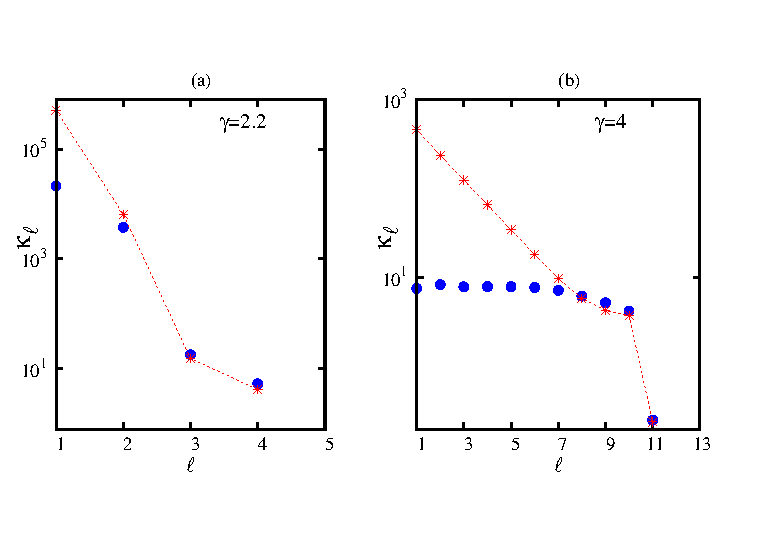
\includegraphics[scale=1,angle=0]{./figures/fig1_1kk}
	\caption{Dépendance de $\kappa_{\ell}$ en $\ell$. Les cercles sont les résultats de la  simulation d'un réseau sans échelle. Les étoiles représentent la simulation du réseau  de la Fig.~\ref{fig1}. Le nombre de nœuds dans les deux cas est $4\times10^6$, chaque point est la moyenne sur $200$ réalisations.}	
	\label{verefication-kappa}
\end{figure}

Selon la construction de la Fig.~\ref{fig1}, le nombre de nœuds entre la première et la $(\ell-1)^{\text{ème}}$ couche est donné par:
\begin{align}
\sum_{j=1}^{\ell-1}n_j&=n\int_{K_{\ell}}^{K_1} P(k)dk \nonumber \\
&=nm^{\gamma-1}(K_{\ell}^{1-\gamma}-K_1^{1-\gamma})\simeq nm^{\gamma-1} K_{\ell}^{1-\gamma},
\label{eq5}
\end{align}
où nous avons utilisé $K_1\gg K_{\ell}$ pour $n$ assez grand. Dans ce cas où $2\textless \gamma \textless 3$, $\kappa_{\ell}\gg 1$, alors
\begin{align}
\sum_{j=1}^{\ell-1}n_j&=\km+\km(\kappa_1-1)+\km(\kappa_1-1)(\kappa_2-1)+\ldots+\km(\kappa_1-1)(\kappa_2-1)\ldots(\kappa_{\ell-1}-2)\nonumber \\
&\approx\km\kappa_1\kappa_2\ldots\kappa_{\ell-2},
\label{eq6}
\end{align}
on en déduit
$K_{\ell}=\Big(\frac{\km\kappa_1\kappa_2\ldots\kappa_{\ell-2}}{nm^{\gamma-1}}\Big)^{\frac{1}{1-\gamma}}$.\\
Le degré moyen de voisins à distance $\ell $ peut maintenant être exprimé comme: 
$\kappa_{\ell}=\frac{\gamma-2}{3-\gamma}m\Big(\frac{n}{\km\kappa_1\kappa_2\ldots\kappa_{\ell-2}}\Big)^{\frac{3-\gamma}{\gamma-1}}$, ce qui conduit à la relation de récurrence $\kappa_{\ell}=\kappa_{\ell-1}
\Big(\kappa_{\ell-2}\Big)^{\frac{\gamma-3}{\gamma-1}}$.  Quand $\gamma$ est dans $]2,3[$ nous avons généralement
$\kappa_{\ell-2} \gg \kappa_{\ell-1}$,  mais puisque $\mid\frac{\gamma-3}{\gamma-1}\mid<1$, on considère alors que $\Big(\kappa_{\ell-2}\Big)^{\frac{\gamma-3}{\gamma-1}}\approx
\Big(\kappa_{\ell-1}\Big)^{\frac{\gamma-3}{\gamma-1}}$. Enfin, on obtient $\kappa_{\ell}=\kappa_1^{\Big(\frac{2\gamma-4}{\gamma-1}\Big)^{\ell-1}}$.\\
Nous pouvons maintenant calculer les sommes dans l'Eq.~\eqref{eq2}:
\begin{align}
\sum_{j=1}^{l} p_jn_j&=\sum_{j=1}^{l}\frac{\kappa_j}{n}\Big(\km\kappa_1\kappa_2\ldots\kappa_{j-1}\Big) \nonumber\\ 
&\approx \frac{\kappa_{\ell}}{n}\Big(\km\kappa_1\kappa_2\ldots\kappa_{\ell-1}\Big) \nonumber \\
&\approx \frac{\km}{n}\kappa_1^{1+\beta+\beta^2+\ldots+\beta^{\ell-1}} \nonumber \\
&\approx \frac{\km}{n}\kappa_1^{\frac{1-\beta^{\ell}}{1-\beta}},
\label{eq7}
\end{align}
où $\beta=\frac{2\gamma-4}{\gamma-1}$. En prenant $n-n_1-1 \approx n$, l'Eq.~\eqref{eq2} peut être écrite pour $2\textless \gamma \textless 3$ comme:
\begin{align}
n_{\ell} &=
\begin{cases}
\km & \text{if}\qquad \ell=1 \\
n\Big(e^{-\frac{\km}{n}\kappa_1^{\frac{1-\beta^{\ell-2}}{1-\beta}}}-e^{-\frac{\km}{n}\kappa_1^{\frac{1-\beta^{\ell-1}}{1-\beta}}}\Big) & \text{if}\qquad \ell \ge 2.
\end{cases}
\label{eq8}
\end{align}
Quand $\gamma> 3 $, les hubs ne sont plus présents, et les propriétés caractéristiques du réseau sont similaires à celles du réseau aléatoire d'ER.
 $\kappa_{\ell}$ est indépendant de $\ell$ comme indiqué dans l'Eq.~\eqref{eq4} et illustré dans la Fig.~\ref{verefication-kappa}, 
alors $\sum_{j=1}^{\ell-1}p_j n_j=\frac{\kappa'}{n}\sum_{j=1}^{\ell-1}n_j$, où $\kappa'=\kappa_1-1$.  
\begin{align}
\sum_{j=1}^{\ell}n_j &=\km+\km(\kappa_1-1)+\km(\kappa_1-1)(\kappa_2-1)+\ldots+\km(\kappa_1-1)(\kappa_2-1)\ldots(\kappa_{\ell-1}-1) \nonumber\\
&=\km+\km\kappa'+\km\kappa'^2+\ldots+\km\kappa'^{\ell-1}=\km\frac{1-\kappa'^{\ell}}{1-\kappa'}. 
\label{eq9}
\end{align}
L'Eq.~\eqref{eq2} s'écrit pour $\gamma>3$ comme:
\begin{align}
n_{\ell} &=
\begin{cases}
\textless k \textgreater & \text{if}\qquad \ell=1 \\
n(e^{-\frac{\textless k \textgreater}{n}\kappa'\frac{1-\kappa'^{\ell-2}}{1-\kappa'}}-e^{-\frac{\km}{n}\kappa'\frac{1-\kappa'^{\ell-1}}{1-\kappa'}}) & \text{if}\qquad \ell \ge 2.
\end{cases}
\label{eq10}
\end{align}
\begin{figure}[h!]
	\centering
	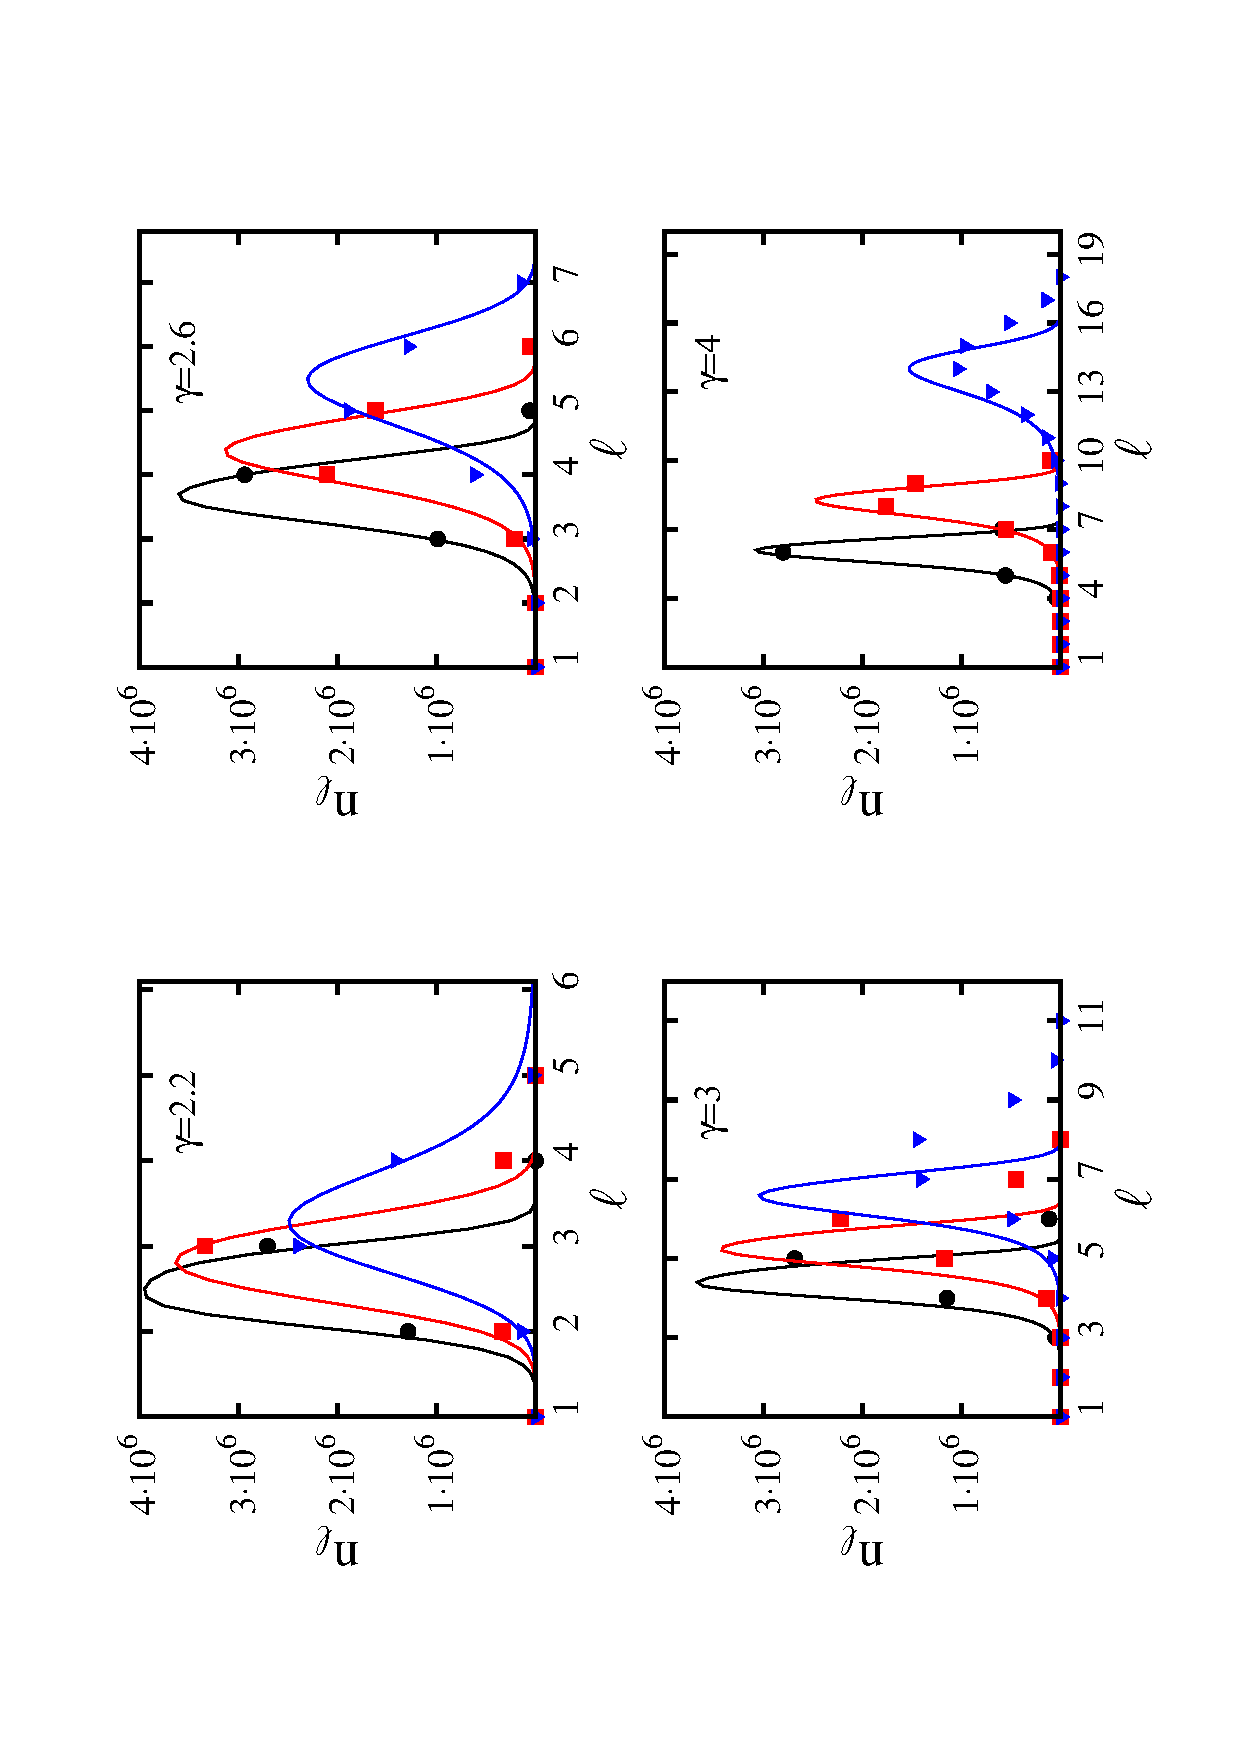
\includegraphics[angle=-90,scale=0.65]{./figures/fig2-3}
	\caption{Nombre de nœuds dans chaque couche pour différentes valeurs de $ \gamma $. Les lignes continues correspondent aux Eq.~\eqref {eq8} et Eq.~\eqref{eq10}. Les symboles sont les simulations numériques d'un réseau de taille $n=4\times10^6$.  Chaque point est la moyenne sur $200$ réalisations. Les couleurs noir, rouge et bleu représentent respectivement les cas $ m = 8, 4 $ et $ 2 $.}
	\label{fig2-3}
\end{figure}

Le cas $\gamma=3$ est le plus problématique. C'est le point où la structure du réseau change radicalement, on passe de la présence de multiples grands hubs et un second moment  $\textless k^2 \textgreater$ qui diverge pour $\gamma<3$, à l'absence de hubs importants et un $\textless k^2  \textgreater$ fini pour $\gamma>3$.
Dans notre approche, le problème se pose lors du calcul de $\sum_{j=1}^{l}p_jn_j$. Néanmoins, en ce point de la transition ($\gamma=3$), certaines propriétés du réseau se comportent presque comme celles pour $\gamma>3$.
Principalement, le plus court chemin est de l'ordre de  $\frac {\ln(n)}{\ln(\ln(n))}$ \cite{Bollobas-Riordan2004}, et $\textless k^2  \textgreater$ reste fini. Nous  utilisons, donc, l'Eq.~\eqref{eq10} pour calculer \nl dans ce cas. \\
Dans la Fig.~\ref{fig2-3}, nous représentons \nl en fonction de $\ell$ pour différentes valeurs de $\gamma$ et $m$. En général, un excellent accord entre la théorie et les simulations est observé. Pour $\gamma=3$, l'accord est moins bon, principalement due au fait que le réseau est encore hétérogène et que les hubs sont toujours présents, alors que nous avons supposé l'homogénéité du réseau pour calculer $\sum_{j=1}^{l} p_jn_j$ dans l'Eq.~\eqref{eq9}. Nous observons aussi une légère  différence  entre la théorie et les simulations lorsque $\gamma=4$ et $m=2$. Ceci est à cause de l'augmentation relative de la proportion de cycles dans les mêmes couches. Ainsi, la structure arborescente parfaite, qui est l'hypothèse principale dans le calcul de \nl, n'est pas très vérifiée. La Fig.~\ref{fig3-3} montre clairement l'importance relative des cycles pour les petites valeurs de $m$. Cet effet est accentué au fur et à mesure qu'on augmente $\gamma$.\\
\begin{figure}[h]
	\begin{center}
		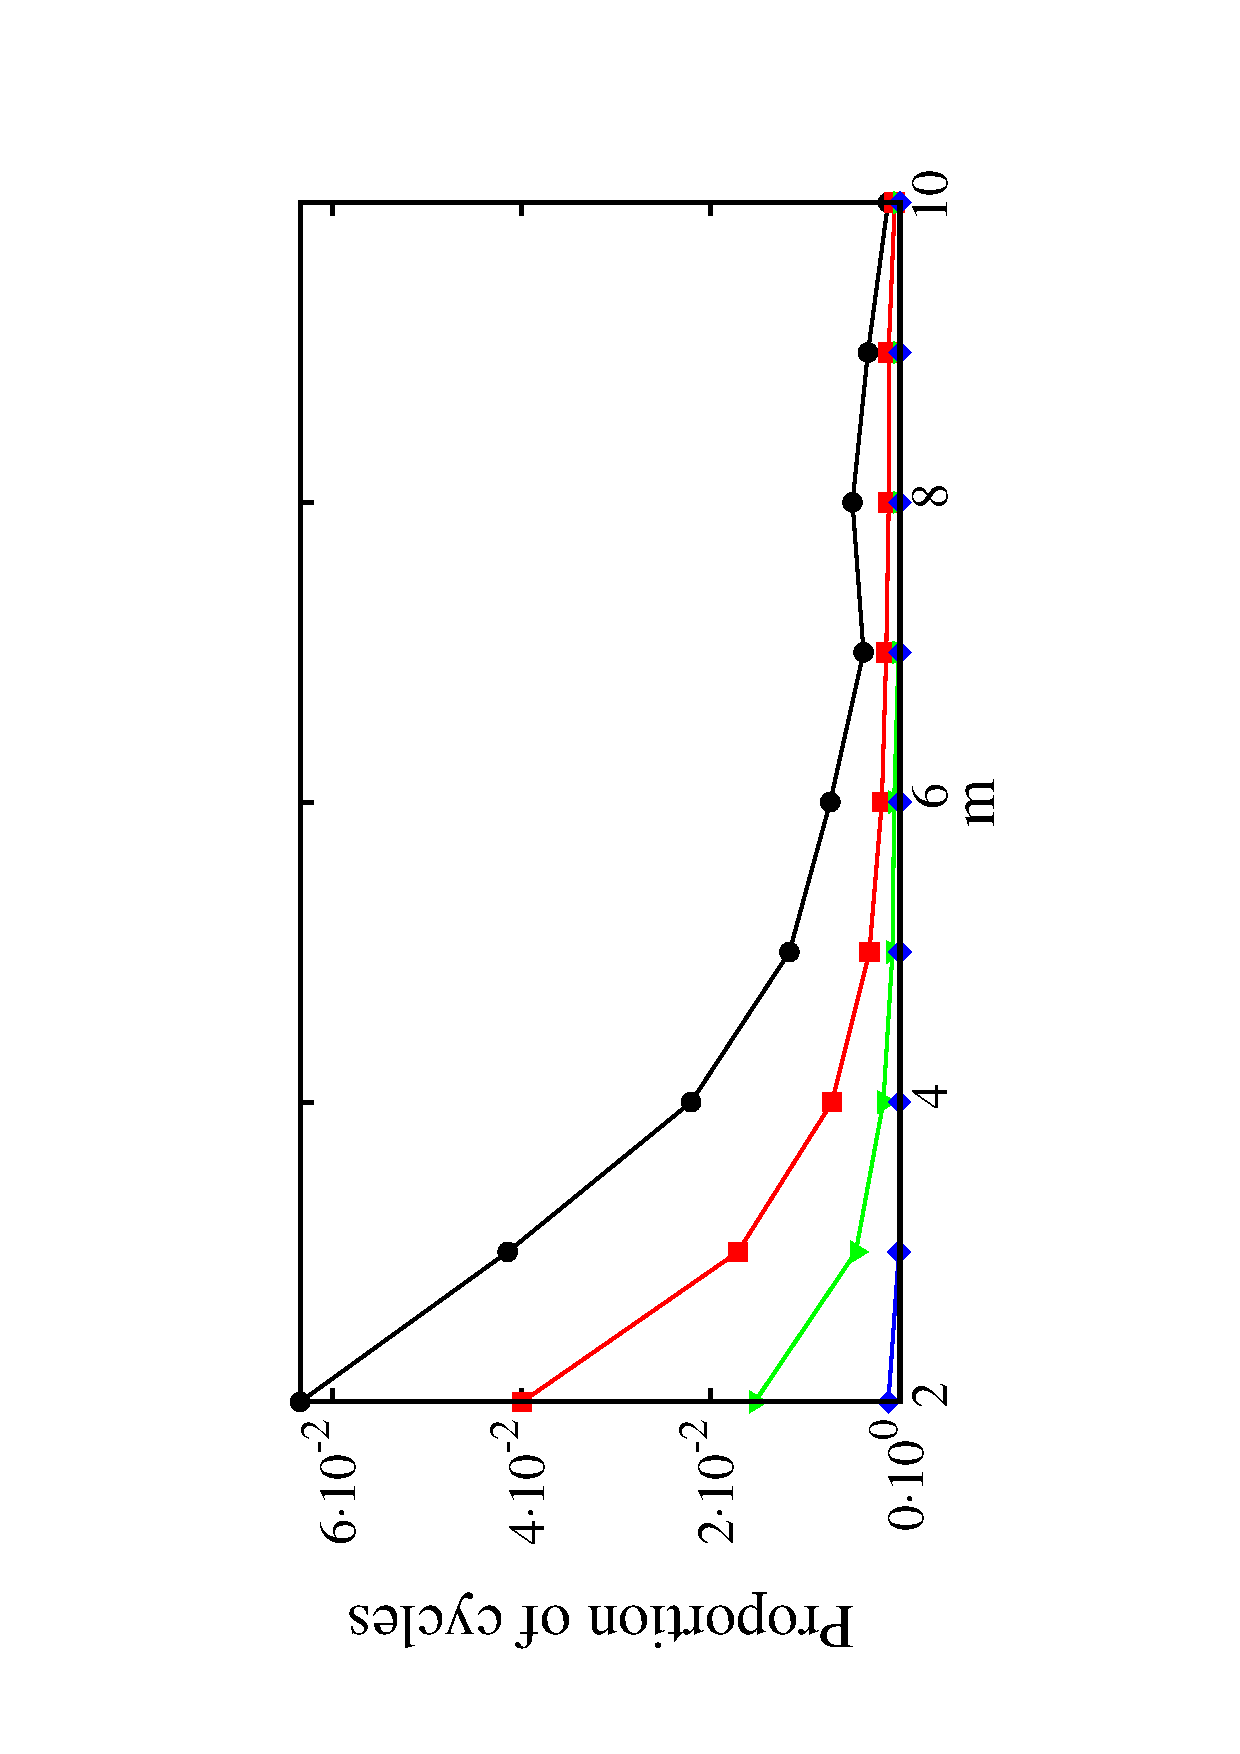
\includegraphics[angle=-90,scale=0.5]{./figures/fig3-3}
	\end{center}
	%\vspace{-10mm}
	\caption{Proportion de cycles dans les couches par rapport à $ m $. De haut en bas, $ \gamma $ est respectivement $ 4, 3, 2.6 $ et $ 2.2 $. Nombre de nœuds $ n = 4.10^6 $, le nombre de réalisations pour chaque point est $200 $.}
	\label{fig3-3}
\end{figure}
Nous observons (Fig.~\ref{fig2-3}) que \nl possède deux allures différentes lors de la croissance et de la décroissance. Pour extraire une information quantitative, concernant les queues de \nl, à partir des Eq.~\eqref{eq8} et Eq.~\eqref {eq10}, on utilise la règle du point milieu. \\
Pour $n$ grand, lorsque $2\textless \gamma \textless 3$, l'Eq.~\eqref{eq8} pour $\ell>1$ peut être approximée comme:
\begin{align}
n_{\ell}&=n\Big(e^{-\frac{\km}{n}\kappa_1^{\frac{1-\beta^{\ell-2}}{1-\beta}}}-e^{-\frac{\km}{n}\kappa_1^{\frac{1-\beta^{\ell-1}}{1-\beta}}}\Big) \nonumber \\
&\approx -n \frac{\partial \Big(e^{-\frac{\km}{n}\kappa_1^{\frac{1-\beta^{\ell-\frac{3}{2}}}{1-\beta}}} \Big) }{\partial \ell} \nonumber \\
&\approx -\frac {\km \ln(\kappa_1) \ln(\beta)} {1-\beta} \beta^{\ell-\frac{3}{2}} \kappa_1^{\frac{1-\beta^{\ell-\frac{3}{2}}}{1-\beta}}e^{-\frac{\km}{n}\kappa_1^{\frac{1-\beta^{\ell-\frac{3}{2}}}{1-\beta}}}, 
\label{eq11}
\end{align}
où $ \ell-\frac{3}{2} $ est utilisé à la place de $ \ell-1$ pour améliorer la différenciation avec la règle du point milieu. Quand $\kappa_1^{\frac{1-\beta^{\ell-\frac{3}{2}}}{1-\beta}}\ll\frac{n}{\km}$,  $e^{-\frac{\km}{n}\kappa_1^{\frac{1-\beta^{\ell-\frac{3}{2}}}{1-\beta}}}\approx 1$, le terme dominant dans l'Eq.~\eqref{eq11}, $\kappa_1^{\frac{1-\beta^{\ell-\frac{3}{2}}}{1-\beta}}$, peut s'écrire comme $\kappa_1^{\frac{1}{1-\beta}}e^{\frac{-e^{\ln(\kappa_1)(\ell-\frac{3}{2})\ln(\beta)}}{1-\beta}}$. Ce dernier terme montre que \nl croit comme une double exponentielle. Après avoir atteint son maximum en $\kappa_1^{\frac{1-\beta^{\ell-\frac{3}{2}}}{1-\beta}}=\frac{n}{\langle k \rangle}$, le terme dominant dans l'Eq.~\ref{eq11} devient 
$e^{-\frac{\langle k \rangle}{n}\kappa_1^{\frac{1-\beta^{\ell-\frac{3}{2}}}{1-\beta}}}$. Pour $\kappa_1^{\frac{1-\beta^{\ell-\frac{3}{2}}}{1-\beta}}\gg \frac{n}{\langle k \rangle}$, \nl décroît comme une triple exponentielle. \\
De la même manière, dans le cas où $\gamma>3$, l'Eq.~\eqref{eq10} peut s'écrire comme
\begin{align}
n_{\ell}&= n(e^{-\frac{\textless k \textgreater}{n}\kappa'\frac{1-\kappa'^{\ell-2}}{1-\kappa'}}-e^{-\frac{\km}{n}\kappa'\frac{1-\kappa'^{\ell-1}}{1-\kappa'}})\nonumber\\
&\approx n\big(e^{-\frac{\km}{n}\kappa'^{\ell-2}}-e^{-\frac{\km}{n}\kappa'^{\ell-1}}\big)\nonumber\\
&\approx n\frac{\partial e^{-\frac{\km}{n}\kappa'^{\ell-\frac{3}{2}}}}{\partial \ell}\nonumber\\
&\approx\km\ln(\kappa')\kappa'^{\ell-\frac{3}{2}}e^{-\frac{\km}{n}\kappa'^{\ell-\frac{3}{2}}},
\end{align}
En suivant les mêmes démarches que précédemment, on obtient une croissance exponentielle pour \nl lorsque $\kappa'^{\ell-\frac{3}{2}} \ll \frac{n}{\km}$ , et une décroissance en double exponentielle lorsque $\kappa'^{\ell-\frac{3}{2}} \gg \frac{n}{\km}$.\\
Nos résultats montrent que \nl décroît toujours plus rapidement qu'elle croit, ceci a été signalé dans le cas du réseau Internet dans \cite{Kalisky-al2006}.\\
Nos résultats analytiques sont aussi comparés aux réseaux du monde réel (voir Fig.~\ref{couch-reel}). La Fig.~\ref{couch-reel} confirme le bon accord  entre nos équations et le réseau Hollywoodien de $392732$ acteurs.  

\begin{figure}[h!]
	\centering
	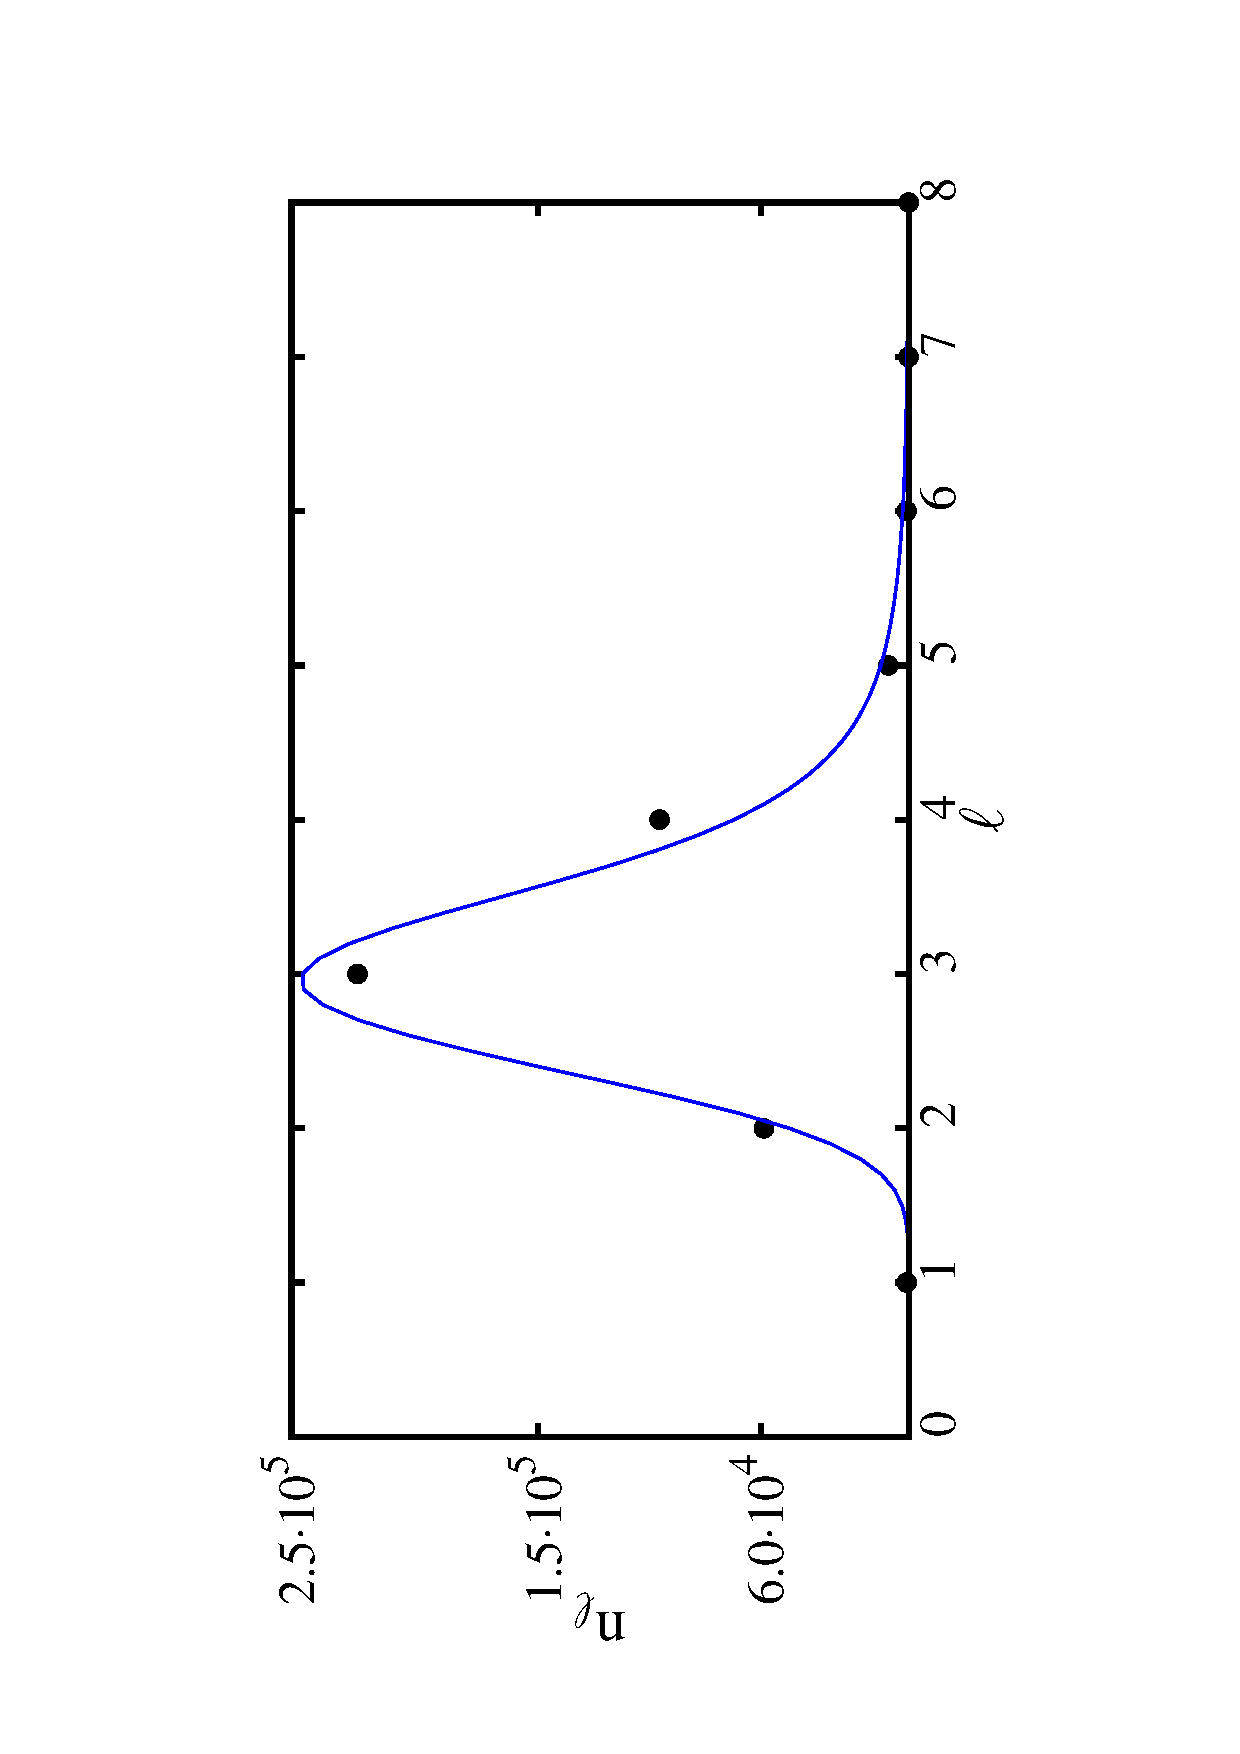
\includegraphics[scale=0.4,angle=-90]{./figures/bacon}
	\caption{Comparaison entre les données empiriques (cercle) et notre théorie (ligne continue): Les cercles représentent les couches du réseau d’acteurs Hollywoodien de $392732$ acteurs avec $\gamma=2.17$. L'acteur Kevin Bacon est au centre du réseau. La ligne continue représente l'Eq.~\eqref{eq8} avec les mêmes valeurs pour $\gamma$ et $n$. Les résultats empiriques ont été extraits du site: "http://oracleofbacon.org/center.php".}	
	\label{couch-reel}
\end{figure}
    
\section{Plus court chemin}
Le plus court chemin, qu'on désignera par $\textless \ell \textgreater$, est peut être le concept le plus intrigant des réseaux complexes, et ce après la célèbre expérience de Milgram \cite{Mi1967}. Dans cette expérience, Milgram a clairement montré l'effet de petit monde dans les réseaux sociaux, ce qui signifie que deux personnes dans le monde, a priori sans aucun lien, sont séparées en moyenne par un nombre petit de  connexions intermédiaires.\\
De nombreux efforts théoriques ont été déployés pour calculer $\textless \ell\textgreater$ \cite{Chung-Lu2002,Do-al2003,Cohen-Havlin2003,Bollobas-Riordan2004,Fronczak-al2004,Chen-al2018,Melnik-Gleeson}, la plupart d’entre eux se sont focalisés sur la manière dont $\textless \ell \textgreater$ varie avec le nombre de nœuds $n$. Dans le Tableau.~\ref{tab1} on résume les principaux résultats dans la littérature.\\
Une expression analytique de la distance moyenne intégrant les paramètres pertinents du réseau est cruciale pour calculer les centralités d'intermédiarité et de proximité, et peut également présenter un grand intérêt pour des situations réelles. Dans le réseau urbain, par exemple, il a été observé que le trafic des véhicules empruntant les voies de communication les plus courtes est celui de la communicabilité \cite{Akbarzadeh-Estrada2018}.\\
Calculer la distance moyenne dans des réseaux complexes est généralement une tâche ardue. Ici, on déduit $\textless \ell \textgreater$ dans un réseau sans échelle non corrélé à partir de la distribution des nœuds, \nl. En fait, la forme quasi symétrique de \nl sur la Fig.~\ref{fig2-3} suggère que $\textless \ell \textgreater$  correspond à la distance où \nl est maximum, ou également, à la distance où $\frac{\partial n_{\ell}}{\partial\ell}=0$.\\ 
\begin{table}[h]
\center
\begin{tabular}{|c|c|c|}
\hline
Valeur de $\gamma$ & Ordre de grandeur & Désignation \\
\hline
$2<\gamma<3$ & $\sim lnln(n)$& ultra-petit monde \cite{Cohen-Havlin2003,Do-al2003,Cohen-al2002,Chung-Lu2002,Fox-Bellwood2014,Hofstad-al2014}\\
\hline
$\gamma=3$ &$\sim \frac{ln(n)}{lnln(n)}$ & petit monde  \cite{Bollobas1985,Chung-Lu2002,Fronczak-al2004,Hofstad-al2004,Cohen-Havlin2009}\\
\hline
$\gamma>3$ &$\sim ln(n)$& petit monde \cite{Bollobas1985,Chung-Lu2002,Fronczak-al2004,Hofstad-al2004,Cohen-Havlin2009}\\
\hline
\end{tabular}
\caption{Principaux résultats sur le plus court chemin en fonction de $\gamma$.}
\label{tab1}
\end{table}
Nous commençons par le cas le plus simple $\gamma=2$. Comme déjà mentionné, il y a un maximum de deux couches dans le réseau, $\textless \ell \textgreater$  s'écrit comme:
   \begin{align}
   	\textless \ell \textgreater=\frac{\km+2(n-\km)}{n},
   	\label{eq14}  
   \end{align}
qui tend vers $2$ pour un grand $n$. Cela signifie que presque tous les nœuds sont connectés entre eux à travers le nœud de degré maximum. \\
Quand $ 2<\gamma<3 $, aucune solution pour $\frac{\partial n_{\ell}}{\partial\ell}=0$ ne peut être trouvée directement à partir de l'Eq.~\eqref{eq8}, alors nous utilisons l'approximation donnée dans l'Eq.~\eqref{eq11}, où \nl est maximum quand $\kappa_1^{\frac{1-\beta^{\textless \ell \textgreater-\frac{3}{2}}}{1-\beta}}=\frac{n}{\km}$. Après avoir remplacé $\kappa_1 $ et $K_1$ par leurs expressions correspondantes, on obtient:
\begin{align}
	\textless \ell \textgreater=\frac{\ln\big(1-\frac{\ln(n)-\ln(\km)}{\ln(n)+\frac{\gamma-1}{3-\gamma}\ln(\frac{\gamma-2}{3-\gamma}m)}\big)}{\ln\big(\frac{2\gamma-4}{\gamma-1}\big)}+\frac{3}{2}.
	\label{eq12}
\end{align}
pour $n$ grand, $\textless \ell \textgreater \approx -\frac{\ln(\ln(n))}{\ln(\beta)}$.
Cette forme d'échelle est derrière la désignation ultra-petit monde \cite{Cohen-Havlin2003}, et elle est largement acceptée pour cet intervalle de $\gamma $ \cite{Do-al2003,Cohen-al2002,Chung-Lu2002,Fox-Bellwood2014,Hofstad-al2014}.\\
Pour $\gamma\ge 3 $, $\textless \ell \textgreater$ peut être déduit de l'Eq.~\eqref{eq10} en résolvant $\frac{\partial n_{\ell}}{\partial\ell}=0$. Cela donne:
\begin{align}
	\textless \ell \textgreater=\frac{\ln (n)}{\ln(\kappa')}+\frac{\ln(\ln(\kappa'))-\ln(\km)}{\ln(\kappa')}+1.
	\label{eq13}
\end{align}
Si $\gamma>3$, $\kappa$ est constant (Eq.~\eqref{eq4}). Pour un grand $n$, $\textless\ell\textgreater\approx\frac{\ln(n)} {\ln(\kappa')}$, qui est la forme d'échelle rapportée dans de nombreux autres travaux \cite{Bollobas1985,Chung-Lu2002,Fronczak-al2004,Hofstad-al2004,Cohen-Havlin2009}, et connu comme l'effet de petit monde. \\
 \begin{figure}[h]
 	\centering
 	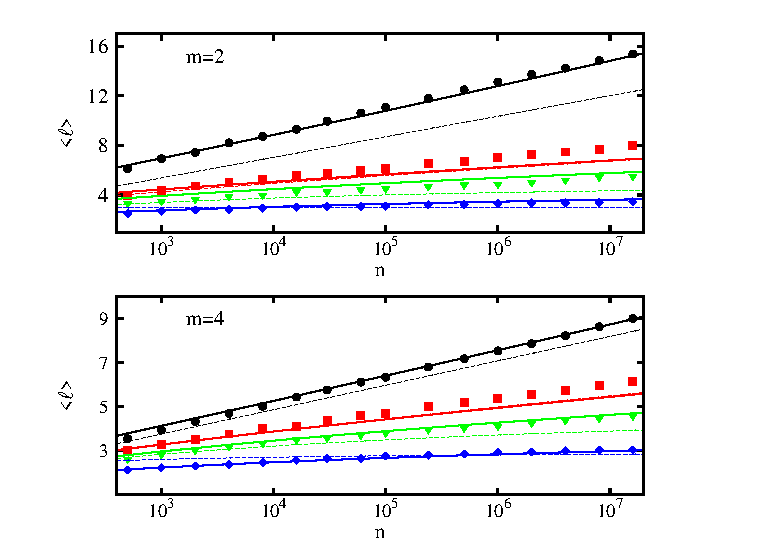
\includegraphics[scale=1.3]{./figures/fig4-3}
 	\caption{Le plus court chemin en fonction du nombre de nœuds. Les valeurs de $\gamma$ de haut en bas sont respectivement $ 4, 3, 2.6 $ et $ 2.2 $. Les lignes continues correspondent à l'Eq.~\eqref{eq12} et à l'Eq.~\eqref{eq13}. Les lignes discontinues correspondent aux équations dans \cite{Fronczak-al2004}. Chaque simulation est moyennée sur plus de $200$ réalisations.}
 	\label{fig4-3}
 \end{figure}
Quand $\gamma=3$, $\kappa$ dépend de $K$, qui dépend à son tour de $n$. Prenant $\kappa_1=m(\ln(K)-\ln(m))$ et $K=mn^{\frac{1}{\gamma-1}}$, nous trouvons pour  $n$ grand, $\textless\ell\textgreater\approx \frac{\ln(n)} {\ln(\ln(n))} $. Ce résultat est en accord avec les travaux précédents \cite {Chung-Lu2002,Cohen-Havlin2003,Fronczak-al2004,Bollobas-Riodan2002}, et confirme le cas particulier de $ \gamma = 3 $. En effet, la présence des hubs rend les distances entre les nœuds plus petites que celles où les hubs sont absents ($\gamma>3$), en même temps les hubs ne sont pas suffisamment grands pour faire des distances ultra-petites comme lorsque $2<\gamma<3$.\\  
Comme nous avons signalé dans la Section.~\ref{PCC}, les travaux importants \cite{Do-al2003,Cohen-Havlin2003} dans ce sujet donnent seulement l'allure de $\textless \ell \textgreater$  pour les grandes valeurs de $n$. L'exception est la contribution de Fronczak et  al. \cite{Fronczak-al2004} où ils ont trouvé des équations fermées en fonction des paramètres du réseau, ces équations prédisent que $\textless \ell \textgreater$  tend vers une valeur constante lorsque $n$ tend vers l'infini pour $2<\gamma<3$, ce qui est en contradiction avec les principaux résultats dans la littérature  \cite{Cohen-Havlin2003,Do-al2003,Cohen-al2002,Chung-Lu2002,Fox-Bellwood2014,Hofstad-al2014}, et avec la simulation numérique (voir Fig.~\ref{fig4-3}).\\ Nos résultats (Fig.~\ref{fig4-3}) montrent un très bon accord avec les simulations pour $\gamma\neq3$. Pour $\gamma=3$,  notre approche donnent des valeurs de $\textless \ell \textgreater$ relativement proches des simulations numériques, et ils sont également très similaires aux résultats de \cite{Fronczak-al2004}.
 \section{conclusion} 
Dans ce chapitre, nous avons étudié en détail certains aspects fondamentaux des réseaux sans échelle non corrélés. \`{A} partir d'arguments probabilistes, nous avons obtenu des expressions explicites, en fonction de l'exposant de degré $\gamma$, pour le nombre de nœuds, \nl, à une distance donnée d'un nœud arbitraire. Nous avons montré que le réseau hétérogène ($2 \textless \gamma \textless 3$) peut être
approximé par un réseau sans échelle ordonné où les nœuds voisins du nœud racine (choisi aléatoirement) sont placés du plus grand au plus petit degré. Ceci peut simplifier les calculs, qui sont en général assez difficiles, dans plusieurs situations des réseaux hétérogènes.\\
Nous avons aussi décrit avec précision les formes des queues de la distribution \nl.\\
Profitant de la forme de celle-ci, nous avons pu déduire les expressions explicites du plus court chemin pour différentes valeurs de $\gamma$. Les expressions obtenues reproduisent les comportements asymptotiques connues pour $n$ grand, à savoir, l'ultra-petit monde pour $2<\gamma<3$, et le petit monde pour $\gamma\ge 3$. Nos résultats théoriques concordent très bien avec les simulations numériques et le nombre de Bacon, sauf dans le cas $\gamma=3$, où nous avons observé la même forme, comme pour les autres valeurs de $\gamma$, dans les queues de \nl, mais avec une notable différence (entre la théorie et la simulation) dans la position du maximum. Cette différence n'affecte pas l'ordre de grandeur du plus court chemin pour cette valeur de $\gamma$.
\let\cleardoublepage\clearpage

% contenu du fichier : chap4.tex
\chapter{Émergence de la propriété petit-monde dans le modèle petit-monde}
%\newcommand{\nl}{$n_{\ell}$ } 
L'émergence de la propriété petit-monde dans le modèle Newman-Watts est encore un phénomène pas bien compris, parmi ses problématiques on cite: à partir de quel point ce réseau change sa nature grand-monde vers petit-monde ? Si ce réseau se sature par les raccourcis ajoutés, comment et quand la saturation se réalise ? Est-ce-qu'il y a vraiment une transition de phase ou non ? Etc.
Par des études théoriques confirmant par une intense nombre de simulations, on abordera quelques questions de ce genre.
\section{Introduction}

Le modèle de Watts-Storogatz (WS) connaît une attention énorme depuis son apparition en 1998 \cite{Watss-Strogatz1998}, il a deux propriétés très intéressantes: la présence d'un coefficient de Clustering élevé et d'un petit PCC. Ces deux propriétés se trouvent dans la plupart des réseaux réels \cite{Cohen-Havlinl2010,Newman2010}, en plus ce modèle est très simple et combine la régularité avec l'aléatoire. En $1999$ Newman et Watts \cite{Newman-Watts1999} ont réalisé une petite modification sur le modèle WS, dont il y a $n$ nœuds qui se distribuent dans un réseau régulier unidimensionnelle sous forme d'une cercle où chaque nœud fait $2k$ liens avec ses plus proches voisins (voir Fig.~\ref{NW}), le nombre de nœuds reste fixe puis chaque lien se reconnecte par une probabilité $\phi$ entre deux autres nœuds choisis aléatoirement sans supprimer aucuns liens, les liens ajoutés sont nommé raccourcis, en moyenne il y a $x=nk\phi$ raccourcis. Ce modèle aussi connaît une grande attention car il a les m\^{e}mes propriétés du modèle WS, sauf pour $k=1$ où il y a une certaine différence\footnote{Le cas $k=1$ ne nous intériorisons jamais dans ce modèle, car dans ce cas le coefficient de Clustering est zéro, alors on prend toujours $k>1$. }, au m\^{e}me temps il est moins difficile dans l'étude.

\begin{figure}[h!]
	\centering 
	\begin{tikzpicture}[scale=0.2]
	\tikzstyle{every node}=[scale=0.4,draw,shape=circle];
	\node[scale=2]  (4) at (-18:8.5) {};
	\node[scale=2] (5) at (0:8.5) {};
	\node[scale=2] (6) at ( 18:8.5) {};
	\node[scale=2] (7) at (2*18:8.5) {};
	\node[scale=2] (8) at (3*18:8.5) {};
	\node[scale=2] (9) at (4*18:8.5) {};
	\node[scale=2] (10) at (5*18:8.5) {};
	\node[scale=2] (11) at (6*18:8.5) {};
	\node[scale=2] (12) at (7*18:8.5) {};
	\node[scale=2] (13) at (8*18:8.5) {};
	\node[scale=2] (14) at (9*18:8.5) {};
	\node[scale=2] (15) at (10*18:8.5) {};
	\node[scale=2] (16) at ( 11*18:8.5) {};
	\node[scale=2] (17) at (12*18:8.5) {};
	\node[scale=2] (18) at (13*18:8.5) {};
	\node[scale=2] (19) at (14*18:8.5) {};
	\node[scale=2] (r) at (15*18:8.5) {};
	\node[scale=2] (1) at (16*18:8.5) {};
	\node[scale=2] (2) at (17*18:8.5) {};
	\node[scale=2] (3) at (18*18:8.5) {};
	\draw[line width=1pt](r)--(1)
	(1) -- (2)
	(2) -- (3)
	(3) -- (4)
	(4) -- (5)
	(5) -- (6)
	(6) -- (7)
	(7) -- (8)
	(8) -- (9)
	(9) -- (10)
	(10) -- (11)
	(11) -- (12)
	(12) -- (13)
	(13) -- (14)
	(14) -- (15)
	(15) -- (16)
	(16) -- (17)
	(17) -- (18)
	(18) -- (19)
	(19) -- (r);
	\draw[line width=1pt] (r) to [bend right=60] (2) 
	(2)to [bend right=60](4)
	(4)to [bend right=60](6)
	(6)to [bend right=60](8)
	(8)to [bend right=60](10)
	(10)to [bend right=60](12)
	(12)to [bend right=60](14)
	(14)to [bend right=60](16)
	(16)to [bend right=60](18)
	(18)to [bend right=60](r)
	
	(1)to [bend right=60](3)
	(3)to [bend right=60](5)
	(5)to [bend right=60](7)
	(7)to [bend right=60](9)
	(9)to [bend right=60](11)
	(11)to [bend right=60](13)
	(13)to [bend right=60](15)
	(15)to [bend right=60](17)
	(17)to [bend right=60](19)
	(19)to [bend right=60](1);
	\end{tikzpicture}
\caption{Un réseau petit-monde WS pour  $n=20$, $k=2$ sans raccourcis.}
\label{NW}
\end{figure}
\begin{sloppypar}
\section{La théorie de groupe de renormalisation et transition de phase}
\end{sloppypar}
Dans un système physique proche d'une transition de phase, les méthodes d'approximations les plus courantes s'appuyant à négliger les corrélations entre un grand nombre de particules ou plutôt entre un grand nombre de degrés de liberté, ces approximations sont valables lorsque la longueur de corrélation est petite. En pratique, on sait traiter de façon simple les corrélations à deux particules. Le problème à trois particules est déjà beaucoup plus difficile. Ce type de méthodes est voué à l'échec quand la longueur de corrélation est grande.

D'où l'idée de réduction du nombre de degrés de liberté, on cherche à établir une correspondance entre un problème de longueur de corrélation donnée et un problème de longueur de corrélation plus petite. La théorie de groupe de renormalisation établit ainsi des correspondances entre systèmes de longueurs de corrélation différentes. Considérons par exemple un système de moments magnétique en interaction au voisinage du point critique de la transition ferromagnétique. Afin de réduire le nombre élevé de degrés de liberté, au lieu de considérer tous les moments magnétiques atomiques individuellement, on les regroupe en blocs comprenant plusieurs moments que l'on considère comme nouvelle entités de base, avec un nouveau moment (moment de bloc). On calcule alors les interactions entre ces nouvelles entités, ce qui suppose que l'on a su moyenner les fluctuations des variables internes à l'intérieur des blocs. On change ensuite d'échelle de façon que le nouveau réseau devient le même que le précédent , enfin, on renormalise judicieusement la taille des nouveaux moments magnétiques. Une série d'opérations fait passer un système à un autre avec réduction de la longueur de corrélation dans un rapport donné. Dans cette transformation, les degrés de liberté du système sont grignotés car on a moyenné les fluctuations des variation internes des blocs. Autrement dit on a remplacé l'interaction initiale entre les anciens degrés de liberté par un nouvelle interaction effective entre les degrés de liberté réduit \cite{Pelissetto-Vicari2002,Wilson1975}.

\section{Plus court chemin et transition de phase dans le modèle NW: ancien contribution et la notre}
\subsection{Ancien contribution}
Malgré tous les  efforts qu'ont été faits, il n'existe pas encore un calcul exact des couches \footnote{ C'est-à-dire le nombre moyen de nœuds, \nl, à distance $\ell$ depuis un nœud arbitraire} et du PCC dans le modèle de NW. En $2000$ Newman, Moore et Watts \cite{Newman-al2000} ont trouvé pour la première fois l'expression de PCC dans ce modèle sous la forme universelle $\ell=\dfrac{n}{k}f(x)$ avec $f$ est la fonction universelle\footnote{Cette fonction universelle a été déjà démontré par Newman et Watts \cite{Newman-Watts1999}, mais sans donné aucune expression théorique, leur étude est basé sur les simulations numériques.}:
\begin{equation}
f(x)=\frac{1}{2\sqrt{x^2+2x}}\tanh^{-1}(\sqrt{\frac{x}{x+2}}),\label{eq-ws}
\end{equation}
 selon NW cette expression est bonne pour le cas de petit nombre des raccourcis et pour les réseaux larges, avec la remarque que au voisinage de $\phi=1$ on observe un déviation entre 
 cette solution analytique et les simulations numériques (voir Fig.~\ref{chemin}). D'une autre coté, le comportement de la transition entre  réseau-régulier et  réseau-aléatoire ou plutôt entre  grand-monde et petit-monde est aussi une part très importante dans l'étude de ce modèle, Barthélémy et Amaral \cite{Barthelemy-Amaral1999} ont trouvé que l'apparition du comportement du petit-monde n'est pas une transition de phase mais un phénomène de croisement, leur méthode tend à déterminer la taille de réseau $n^*(\phi)$ pour lequel: si $n<n^*$, $\ell$ croît linéairement avec $n$, et si $n>n^*$, $\ell$ croît comme $\ln(n)$. Par des analyses numériques ils ont trouvé que $n^*(\phi)\sim\phi^{-\tau}$ avec 
$\tau\approx\frac{2}{3}$. Ces résultats sont rapidement critiqués par Barrat \cite{Barrat} car il a démontré que $\tau$ ne peut pas être inférieur à $1$, en plus il a trouvé que $\tau=1$ en utilisant la m\^{e}me approche de Barthélémy et Amaral mais avec
des tailles de système plus grand. Newman et Watts \cite{Newman-Watts1999-2,Newman-Watts1999-3} confirment cette valeur de l'exposant critique unique $\tau=1$ en utilisant une transformation de groupe de renormalisation et ils ont dit aussi que la transition vers le petit-monde se fait d'une façon continue, c'est-à-dire par une transition de phase de deuxième ordre où le point de transition de phase se réalise lorsque la densité des raccourcis tend vers zéro ($\phi=0$). Mais M. Argollo et al. \cite{Argollo-al2000} ont obtenu que la transition de phase
est de première ordre au point $\phi=0$, à cause d'une discontinuité d'un certain paramètre d'ordre dans ce point. On en déduit qu'il y a  encore un débat à propos du type de transition de phase dans ce modèle.
\subsection{Notre contribution}
Notre travail ici se consacre, au début, à faire une étude sur les couches dans le modèle NW en utilisant la transformation de groupe de renormalisation en espace réel (GR), (voir Fig.~\ref{RG}). Une couche $n_d$ est le nombre de nœuds ayant la distance $d$ autour d'un nœud arbitraire. Sachant que ce modèle est un mélange entre la régularité et l'aléatoire,
nous proposons de séparer les couches selon deux types, couches-régulières $n_d^r$ qui représentent les nœuds restant dans leurs distances régulières initiales, $d$, sans aucune influence par les raccourcis ajoutés et les  couches-aléatoires $n_d^{al}$ qui représentent les nœuds changeant leurs distances régulières vers une autre 
plus proche de nœud arbitraire, $d$, à cause des raccourcis (voir Fig.~\ref{r-al}). En manipulant les expressions de ces couches, on trouvera que la somme des couches aléatoires $S_{al}$ et la somme des couches régulières $S_{r}$, pouvant également s'écrire sous  forme d'une fonction universelle comme le PCC, $S_{al}=nh(x)$ et $S_{r}=n(1-h(x))$ avec $h(x)=1-\sqrt{\frac{\pi}{4x}}erf(\sqrt{x})$. 
Sachant que la fonction $h(x)$ représente la fraction des nœuds appartient aux couches-aléatoires, on peut la considérer comme un
paramètre d'ordre, car il varie entre $0$ et $1$ selon le degré de l'ordre et de désordre dans le réseau. A partir de l'expression de $h(x)$ on déduit l'absence d'une transition de phase dans ce modèle mais un phénomène de croisement qui commence depuis $x=0$.\\

Pour calculer le PCC, $\ell$, 
nous utilisons les résultats précédent et nous prenons également, comme le cas des couches, que le PCC est la somme de PCC de réseau-régulier $\ell_{r}$ et le PCC de réseau-aléatoire  $\ell_{al}$, $\ell=\ell_{al}+\ell_r$, en se
 basant dans le calcul de $\ell_{al}$ sur la proposition que le PCC est la position de la couche maximale (voir Chapitre.~\ref{sec3}) et pour calculer $\ell_r$ on utilise une approximation qui sera décrite dans la troisième section de ce chapitre, et on va trouver une expression de PCC  plus précise par rapport à l'expression de Newman et al. (voir Fig.~\ref{chemin}).
En plus on va démontrer que la formule universelle en fonction de nombre de raccourcis est valable sauf pour $y\ll1$, avec $y=2k\phi$ un paramètre qu'on va définir plus tard. Ce résultat est très important, car on a montré que la fonction  universelle $f(x)$ qui a été considéré conceptuellement vrai n'est pas toujours valable, en revanche on obtient une autre formule universelle $g(y)$ qui est valable lorsque  $y$ n'est pas très inférieur à $1$. Cette nouvelle formule sous la forme $g(y)=\frac{ln(n)}{\ell}$, nous montre que la propriété petit-monde émerge d'une façon universelle en fonction de $y$.

\section{Structure de réseau NW: couche et plus court chemin }

\subsection{Les couches aléatoires et régulières}
Au début on va appliquer une transformation de groupe de renormalisation en espace réel, en transformant le réseau NW de $k$ et $n$ quelconque à un réseau de $\acute{k}=1$ et de nombre de nœuds {$\acute{n}$}$=\frac{n}{k}$ 
(voir Fig.~\ref{RG})\footnote{On voit que le degré de liberté est réduit, car dans le nouveau réseau le paramètre  $\acute{k}$  est toujours égale à $1$, c'est exactement l'idée de la théorie de groupe de renormalisation.}. On suppose que chaque ensemble de $k$ nœuds voisins comme un seul nœud,  d'où la probabilité qu'un
nœud dans le nouveau réseau ($\acute{k}=1$ et $\acute{n}=\frac{n}{k}$) est lié aléatoirement à un autre nœud est $q=1-\big(1-\frac{2k\phi}{n}\big)^{k^2}$, pour $n\gg k\phi$ on peut écrire $q=\frac{2k^3\phi}{n}$. Puis nous calculons la probabilité $P_r(j)$ qu'un nœud reste dans sa distance régulière $j$ et la probabilité $P_{al}(j)$ qu'un nœud change sa distance régulière vers une nouvelle distance $j$ plus proche de nœud arbitraire grâce aux raccourcis ajoutés, par exemple, dans la Fig.~\ref{r-al}, les nœuds noires sont celles qui devient plus proche de nœud arbitraire grâce au raccourci.\\ Généralement les recules des nœuds vers des distances plus
proche de nœud arbitraire se fassent à travers $1$ raccourci, $2$ ou plus, pour cette raison on distingue chaque cas différemment.\\
\begin{figure}[h!]
\centering
\begin{tikzpicture}[scale=0.25]
\tikzstyle{every node}=[scale=0.5,draw,shape=circle];
\node[scale=2,fill=black] (4) at (-18:9) {};
\node[scale=2,fill=black] (5) at (0:9) {};
\node[scale=2,fill=black] (6) at ( 18:9) {};
\node[scale=2,fill=black] (7) at (2*18:9) {};
\node[scale=2,fill=black] (8) at (3*18:9) {};
\node[scale=2,fill=black] (9) at (4*18:9) {};
\node[scale=2,fill=black] (10) at (5*18:9) {};
\node[scale=2,fill=black] (11) at (6*18:9) {};
\node[scale=2,fill=black] (12) at (7*18:9) {};
\node[scale=2] (13) at (8*18:9) {};
\node[scale=2] (14) at (9*18:9) {};
\node[scale=2] (15) at (10*18:9) {};
\node[scale=2] (16) at ( 11*18:9) {};
\node[scale=2] (17) at (12*18:9) {};
\node[scale=2] (18) at (13*18:9) {};
\node[scale=2] (19) at (14*18:9) {};
\node[scale=1.3] (r) at (15*18:9) {R};
\node[scale=2] (1) at (16*18:9) {};
\node[scale=2] (2) at (17*18:9) {};
\node[scale=2] (3) at (18*18:9) {};
\draw[line width=1.5pt](r)--(1)
(1) -- (2)
(2) -- (3)
(3) -- (4)
(4) -- (5)
(5) -- (6)
(6) -- (7)
(7) -- (8)
(8) -- (9)
(9) -- (10)
(10) -- (11)
(11) -- (12)
(12) -- (13)
(13) -- (14)
(14) -- (15)
(15) -- (16)
(16) -- (17)
(17) -- (18)
(18) -- (19)
(19) -- (r)
(r) -- (6);
\end{tikzpicture}
\caption{ Illustration des nœuds aléatoires (nœuds noires) qui devient plus proche du nœud arbitraire $R$, et nœuds réguliers (nœuds blanches) qui restent dans leurs distance initial par rapport au même nœud arbitraire $R$, le réseau est de taille $n=20$, $k=1$ et un seul raccourci.}

\label{r-al}
\end{figure}
\begin{itemize}
\item[$\blacksquare$]  \`{A} travers $1$ raccourci:\\
Soit $\pi^1(i)$ la probabilité qu'un nœud ne change pas sa distance régulière $j$ vers
la $i^{\text{ème}}$ distance ($i<j$) à travers un seul raccourci:
\begin{eqnarray}\nonumber
	\pi^1(1)&=&(1-q), \\\nonumber
	\pi^1(2)&=&(1-q)^4,\\\nonumber
	\pi^1(3)&=&(1-q)^{4\cdot2},\\\nonumber
	\vdots\\
	\pi^1(i)&=&(1-q)^{4(i-1)}.
	\label{pi1}
	\end{eqnarray}
	Il faut signalé que l'expression $\pi^1(i)=(1-q)^{4(i-1)}$ est une approximation de champs moyenne qu'est vrai pour la plupart des cas et qui représente la valeur minimale de cette probabilité, car les nombres des possibilités
	$4,4\times2,...,4\times(i-1)$ sont les valeurs maximales, mais à cause des interférences entres elles, le nombre de possibilités peut être moindre, la m\^{e}me remarque pour tous les cas 
	suivants, on prend toujours le nombre maximum de possibilité, d'où nos équations sont des approximations de champs moyenne et ne sont pas des expressions 
	mathématiques exactes, certes comme tous les systèmes de très grand nombre de constituants, il suffit de faire la bonne 
	approximation au niveau microscopique, c'est-à-dire local, pour trouver la description parfaite des grandeurs macroscopique de système, ce que nous
	avons exactement fait.\\
	De l'Eq.~\eqref{pi1} la probabilité $P^1_r(j)$ qu'un nœud ne change pas sa distance régulière $j$ à travers un seul raccourci est:
	\begin{eqnarray}\nonumber
	P_r^1(j)&=&\pi^1(1)\pi^1(2)...\pi^1(j-1)\\\nonumber
	&=& (1-q)(1-q)^4(1-q)^{4\cdot2}...(1-q)^{4(j-2)}\\\nonumber
	&=&(1-q)^{1+4+4\cdot2+4\cdot3...4(j-2)}\\\nonumber
	&=&(1-q)^{1+4\sum_{i=1}^{j-1}(i-1)}.
	\end{eqnarray}
	On doit signaler qu'on peut négliger le cas $\pi^i(i)=(1-q)^{i}(\acute{n}-2i)^{i-1}$,  dans le cas d'un raccourci et dans tous les cas suivants sans aucun problème, alors $P_r^1(j)$ sera écrite:
	$$P_r^1(j)=(1-q)^{4\sum_{i=1}^{j-1}(i-1)}$$
	
\item[$\blacksquare$]  \`{A} travers $2$ raccourcis: \\
La probabilité qu'un nœud ne change pas sa distance régulière $j$ vers la $i^{\text{ème}}$ distance ($i<j$) à travers deux raccourcis, dans
le cas où le nœud arbitraire lié directement par un raccourci avec un nœud intermédiaire $z$ qui est à une distance $i-1$ du
nœud $j$ à travers aussi un seul raccourci, est $(1-q^2)^{4(i-2)}$. On considère que cette probabilité est la m\^{e}me
pour les autres possibilités d'arrangements de deux  raccourcis autour le nœud intermédiaire.\\ Le nombre
possible des arrangements de ces deux raccourcis autour de nœud intermédiaire $z$ pour lequel la distance entre $j$ et le nœud arbitraire sera toujours $i$ est\footnote{Par exemple dans le cas où $i=4$, on a $3$ des arrangements possibles pour que la distance entre le nœud $j$ et le nombre arbitraire est $4$:\\ le $1^{\text{ère}}$: la distance entre le nœud arbitraire et le nœud intermédier $z$ est $1$ et entre $z$ et le nœud $j$ est $3$.\\ le $2^{\text{ème}}$: la distance entre le nœud arbitraire et le nœud intermédier $z$ est $2$ et entre $z$ et le nœud $j$ est également $2$.\\ le $3^{\text{ème}}$: la distance entre le nœud arbitraire et le nœud intermédier $z$ est $3$ et entre $z$ et le nœud $j$ est $1$.}  $(i-1)$.\\
En outre le nombre maximal possible des positions de $z$ sur le réseau pour que $i<j$ est
$\acute{n}-2i$, alors la probabilité qu'un nœud ne change pas sa distance régulière $j$ vers
la $i^{\text{ème}}$ distance ($i<j$) à travers deux raccourcis est
\begin{eqnarray}
	\pi^2(i)=(1-q^2)^{4(i-1)(i-2)(\acute{n}-2i)},\nonumber
\end{eqnarray}
d'où
\begin{eqnarray}
	P_r^2(j)&=&\pi^2(1)\pi^2(2)...\pi^2(j-1)\\\nonumber
	&=& (1-q^2)^{4\sum_{i=1}^{i=j-1}((i-1)(i-2)(\acute{n}-2i))},
\end{eqnarray}
comme nous avons déjà signalé le terme $\pi^i(i)$ est négligeable, ici est $\pi^2(2)$.\\
	
\item[$\blacksquare$]  \`{A} travers $3$ raccourcis:\\
	Dans ce cas on a deux nœuds intermédiaires $z$ et $\acute{z}$ sous la condition que entre deux nœuds intérimaires il y a un seul raccourci.
	La probabilité qu'un nœud ne change pas sa distance $j$ vers la $i^{\text{ème}}$ distance à travers $3$ raccourcis pour le cas où le
	nœud arbitraire lié directement par un raccourci avec $z$ qui lié aussi directement par un raccourci avec $\acute{z}$ et ce 
	dernière à une distance de $i-2$ au nœud $j$ à travers aussi un seul raccourci, est $(1-q^3)^{4(i-3)}$. On considère que cette probabilité est la m\^{e}me
	pour les autres possibilités d'arrangements de trois raccourcis autour les deux nœuds intermédiaires.\\
	Le nombre possible des
	arrangements de ces trois raccourcis autour des nœuds intérimaires $z$ et $\acute{z}$ pour que la distance entre $j$ et le	nœud arbitraire est toujours $i$ est $C_2^{i-1}=\frac{(i-1)(i-2)}{2!}$.\\
	 En outre le nombre maximal possible des positions de $z$ et
	$\acute{z}$ sur le réseau pour $i<j$ est approximativement $(\acute{n}-2i)^2$.\\
	
	Alors on obtient que $\pi^3(i)=(1-q^3)^{4\frac{(i-1)(i-2)}{2!}(i-3)(\acute{n}-2i)^2}\nonumber$ d'où
	\begin{eqnarray}
	P_r^3(j)&=&\pi^3(1)\pi^3(2)...\pi^3(j-1)\\\nonumber
	&=& (1-q^3)^{4\sum_{i=1}^{i=j-1}(\frac{(i-1)(i-2)}{2!}(i-3)(\acute{n}-2i)^2)}.
	\end{eqnarray}
	
\item[$\blacksquare$] \`{A} travers $4$ raccourcis:\\
Dans ce cas on a trois nœuds intermédiaires $z$,$z'$ et $z''$, toujours sous la condition  qu'il y a un seul raccourci entre chaque deux nœuds
intérimaires. La probabilité qu'un nœud ne change pas sa distance $j$ vers la $i^{\text{ème}}$ distance à travers $4$ raccourcis pour 
le cas où le nœud arbitraire lié directement par un raccourci avec $z$ et celui-ci lié également directement par un raccourci 
avec $z'$ qui est de sa part lié directement par un raccourci avec le nœud $z''$  et ce dernier à une distance de $i-3$ au
nœud $j$ à travers aussi un seul raccourci est $(1-q^4)^{4(i-4)}$.
On considère comme les cas précédent que cette probabilité est la m\^{e}me
pour les autres possibilités d'arrangements de quatre raccourcis autour les trois nœuds intermédiaires.\\ Le nombre possible des arrangements de ces trois raccourcis
autour des nœuds intérimaires $z$,$z'$ et $z''$ pour que la distance entre $j$ et le nœud  arbitraire est $i$ est
$C_3^{i-1}=\frac{(i-1)(i-2)(i-3)}{3!}$.\\ En outre le nombre maximal possible  des positions de $z$,$z'$ et $z''$ sur le réseau pour $i<j$ est  approximativement
$(\acute{n}-2i)^3$.
Alors on obtient
\begin{eqnarray}
	\pi^4(i)=(1-q^4)^{4\frac{(i-1)(i-2)(i-3)}{3!}(i-4)(\acute{n}-2i)^3},\nonumber
	\end{eqnarray}
	d'où
	\begin{eqnarray}
	P_r^4(j)&=&\pi^4(1)\pi^4(2)...\pi^4(j-1)\\\nonumber
	&=& (1-q^4)^{4\sum_{i=1}^{i=j-1}(\frac{(i-1)(i-2)(i-3)}{3!}(i-4)(\acute{n}-2i)^3)}.
	\end{eqnarray}
	
\item[$\blacksquare$] \`{A} travers $m$ raccourcis:\\
Par la m\^{e}me méthode, si on suppose qu'il  y a $(m-1)$ nœuds intermédiaires, on va obtenir l'expression générale de la probabilité qu'un nœud ne change pas sa distance $j$ vers la $i^{\text{ème}}$ distance à travers $m$ raccourcis sous la forme 
\begin{eqnarray}
	\pi^m(i)=(1-q^m)^{4\frac{(i-1)(i-2)\ldots(i-m)}{(m-1)!}(\acute{n}-2i)^{(m-1)}},\nonumber
\end{eqnarray}
alors la probabilité qu'un nœud ne change pas sa distance régulière $j$ à travers $m$ raccourcis est
\begin{eqnarray}
	P_r^m(j)&=&\pi^m(1)\pi^m(2)...\pi^m(j-1)\\\nonumber
	&=& (1-q^m)^{4\sum_{i=1}^{j-1}(\frac{(i-1)(i-2)\ldots(i-m)}{(m-1)!}(\acute{n}-2i)^{m-1})},
	\end{eqnarray}
sachant que $q<1$ on peut écrire 
\begin{eqnarray}
P_r^m(j)=e^{-4q^m\sum_{i=1}^{j-1}(\frac{(i-1)(i-2)\ldots(i-m)}{(m-1)!}(\acute{n}-2i)^{m-1})}.
\end{eqnarray}
\end{itemize}

Alors la probabilité $P_r(j)$ qu'un nœud ne change pas sa distance régulière $j$ vers la $i^{\text{ème}}$ distance par n'importe 
quel nombre des raccourcis est
\begin{eqnarray}
P_r(j)&=&P^1_r(j)P^2_r(j)P^4_r(j)\ldots P^m_r(j)\\\nonumber
&=&e^{-4q\sum_{i=1}^{j-1}(i-1)B(i)}, 
\end{eqnarray}
avec $B(i)=\big(1+[q(i-2)(\acute{n}-2i)]+[q^2\frac{(i-2)(i-3)}{2!}(\acute{n}-2i)^{2}]+\ldots+[q^{m-1}\frac{(i-2)\ldots
	(i-m)}{(m-1)!}(\acute{n}-2i)^{m-1}]+\ldots+[q^{i-2}(\acute{n}-2i)^{i-2}]\big)$, les termes de cette expression lient respectivement
au probabilité que le nœud $j$ ne change pas sa distance vers le $i^{\text{ème}}$ distance par $2,3,4,...,i-1$ raccourcis, le cas de $i$ 
raccourcis est négligé comme nous avons déjà dit. D'une autre coté on voit que $B(i)$ peut s'écrire sous la formule du Bin\^{o}me
\begin{eqnarray}\nonumber
B(i)&=&\big(1+[q(i-2)(\acute{n}-2i)]+[q^2\frac{(i-2)(i-3)}{2!}(\acute{n}-2i)^{2}]+\ldots+[q^{i-2}(\acute{n}-2i)^{i-2}]\big)\\\nonumber
&=&\sum_{j=1}^{i-2}C_j^{i-2}[q(\acute{n}-2i)]^j1^{i-2-j}\\\nonumber
&=&(q(\acute{n}-2i)+1)^{i-2}.
\end{eqnarray}

\begin{figure}[h!]
	\centering 
\begin{tikzpicture}[scale=0.2]
\draw (0,-12) node[scale=2,below]{$a)$} ;
\tikzstyle{every node}=[scale=0.5,draw,shape=circle];
\node[scale=2]  (4) at (-18:8.5) {};
\node[scale=2,fill=black] (5) at (0:8.5) {};
\node[scale=2,fill=black] (6) at ( 18:8.5) {};
\node[scale=2] (7) at (2*18:8.5) {};
\node[scale=2] (8) at (3*18:8.5) {};
\node[scale=2,fill=black] (9) at (4*18:8.5) {};
\node[scale=2,fill=black] (10) at (5*18:8.5) {};
\node[scale=2] (11) at (6*18:8.5) {};
\node[scale=2] (12) at (7*18:8.5) {};
\node[scale=2,fill=black] (13) at (8*18:8.5) {};
\node[scale=2,fill=black] (14) at (9*18:8.5) {};
\node[scale=2] (15) at (10*18:8.5) {};
\node[scale=2] (16) at ( 11*18:8.5) {};
\node[scale=2,fill=black] (17) at (12*18:8.5) {};
\node[scale=2,fill=black] (18) at (13*18:8.5) {};
\node[scale=2] (19) at (14*18:8.5) {};
\node[scale=2] (r) at (15*18:8.5) {};
\node[scale=2,fill=black] (1) at (16*18:8.5) {};
\node[scale=2,fill=black] (2) at (17*18:8.5) {};
\node[scale=2] (3) at (18*18:8.5) {};
\draw[line width=1pt](r)--(1)
(1) -- (2)
(2) -- (3)
(3) -- (4)
(4) -- (5)
(5) -- (6)
(6) -- (7)
(7) -- (8)
(8) -- (9)
(9) -- (10)
(10) -- (11)
(11) -- (12)
(12) -- (13)
(13) -- (14)
(14) -- (15)
(15) -- (16)
(16) -- (17)
(17) -- (18)
(18) -- (19)
(19) -- (r);
\draw[line width=1pt] (r) to [bend right=60] (2) 
(2)to [bend right=60](4)
(4)to [bend right=60](6)
(6)to [bend right=60](8)
(8)to [bend right=60](10)
(10)to [bend right=60](12)
(12)to [bend right=60](14)
(14)to [bend right=60](16)
(16)to [bend right=60](18)
(18)to [bend right=60](r)

(1)to [bend right=60](3)
(3)to [bend right=60](5)
(5)to [bend right=60](7)
(7)to [bend right=60](9)
(9)to [bend right=60](11)
(11)to [bend right=60](13)
(13)to [bend right=60](15)
(15)to [bend right=60](17)
(17)to [bend right=60](19)
(19)to [bend right=60](1);
\end{tikzpicture}
\begin{tikzpicture}[scale=0.22]
\draw (0,-12) node[scale=1.8,below]{$b)$} ;
\tikzstyle{every node}=[scale=0.5,draw,shape=circle];
\node (4)[scale=2] at (-36:8.5) {};
\node (5)[scale=2,fill=black]  at (0:8.5) {};
\node (6)[scale=2] at ( 36:8.5) {};
\node (7)[scale=2,fill=black]  at (2*36:8.5) {};
\node (8)[scale=2] at (3*36:8.5) {};
\node (9)[scale=2,fill=black]  at (4*36:8.5) {};
\node (r)[scale=2] at (15*36:8.5) {};
\node[scale=2,fill=black] (1) at (16*36:8.5) {};
\node (2)[scale=2] at (17*36:8.5) {};
\node[scale=2,fill=black]  (3) at (18*36:8.5) {};
\draw[line width=1pt](r)--(1)
(1) -- (2)
(2) -- (3)
(3) -- (4)
(4) -- (5)
(5) -- (6)
(6) -- (7)
(7) -- (8)
(8) -- (9)
(9) -- (r);
%\node[scale=3,text centered] at (0,-12) {b)};
\end{tikzpicture}
\caption{La transformation GR d'un réseau (a) de $n=20$ et $k=2$ vers un réseau (b) de $\acute{n}=10$ et $\acute{k}=1$.}
\label{RG}
\end{figure}
Alors la probabilité qu'un nœud ne change pas sa distance $j$ est: 
\begin{eqnarray}
\label{pr}
P_r(j)&=& e^{-4q\sum_{i=1}^{j-1}(i-1)(q(\acute{n}-2i)+1)^{i-2}}\\\nonumber
&=&e^{-4q\int_{i=1}^{j-1}(i-1)(q(\acute{n}-2i)+1)^{i-2}di}.
\end{eqnarray}

En outre la probabilité $P_{al}(j)$ qu'un nœud change sa distance régulière vers la  $j^{\text{ème}}$ égale le produit de la probabilité que ce nœud ne change pas sa distance vers une autre inférieur à  $j$, $P_r(j-1)$, et la probabilité que le nœud change sa distance vers la $j^{\text{ème}}$ distance,$1-\pi(j)$,
\begin{eqnarray}\nonumber
P_{al}(j)&=&P_r(j-1)(1-\pi(j))\\\nonumber
&=&P_r(j-1)-\pi(j)P_r(j-1)\\\nonumber
&=&P_r(j-1)-P_r(j)\\\nonumber
&=&-\frac{\partial P_r(j)}{\partial j}\\
&=&4q(j-2)(q(\acute{n}-2(j-1)-1))+1)^{j-3}P_r(j),
\end{eqnarray}
pour simplifier les calculs on peut prendre sans aucun souci\footnote{Cette approximation signifie une augmentation de l'erreur de l'ordre $\frac{1}{\ell}$, cependant $\ell$ tend vers l'infini lorsque $n$ est très large, alors cette approximation ne pose aucun problème.} que dans l'équation précédent $j-1=j$, d'où on obtient
\begin{eqnarray}
P_{al}(j)=4q(j-1)(q(\acute{n}-2j-1))+1)^{j-2}P_r(j).
\label{pal}
\end{eqnarray}
Le nombre des nœuds dans la couche $n_{j}^r$ est $P_r(j)$ multiplié par $2$, car initialement dans chaque couche on a  deux nœuds réguliers
\begin{eqnarray}
n_{j}^r=2P_r(j),
\label{cr}
\end{eqnarray}
et le nombre des nœuds dans le couche aléatoire $n_{j}^{al}$ est $P_{al}(j)$ multiplié par le nombre des nœuds qui ont une distance plus grande que $j$
\begin{eqnarray}
n_{j}^{al}=(\acute{n}-2j)P_{al}(j),
\label{cal}
\end{eqnarray}
d'où la $j^{\text{ème}}$ couche est
\begin{eqnarray}
n_j&=&n_{j}^{r}+n_{j}^{al}\\\nonumber
&=&2P_r(j)+(\acute{n}-2j)P_{al}(j)\\\nonumber
&=&2P_r(j)+(\acute{n}-2j)P_r(j-1)-(\acute{n}-2j)P_r(j)\\\nonumber
&=&(\acute{n}-2j)P_r(j-1)-(\acute{n}-2(j+1))P_r(j)\\\nonumber
&=&v(j-1)-v(j) \quad \quad  \text{avec:} \quad v(j)=(\acute{n}-2(j+1))P_r(j).
\nonumber
\label{c}
\end{eqnarray}
Maintenant on va calculer la somme des nœuds de couches-régulières $S'_r$ et la somme des nœuds de couches-aléatoires $S'_{al}$ afin de les utiliser dans le calcul de PCC. De Eq.~\eqref{pr} et Eq.~\eqref{cr} on obtient

\begin{eqnarray}
S'_r &=&n_{1}^{r}+\sum^{\frac{\acute{n}}{2}}_2n_{i}^{r}\\\nonumber
&=&n_{1}^{r}+\int^{\frac{\acute{n}}{2}}_2n_{i}^{r}di\\\nonumber
&=&n_{1}^{r}+2\int^{\frac{\acute{n}}{2}}_2e^{-4q\int_{j=1}^{i-1}(j-1)(q(\acute{n}-2j)+1)^{j-2}dj}di,\nonumber
\end{eqnarray}
l'intégrale $\int^{\frac{\acute{n}}{2}}_2e^{-4q\int_{j=1}^{i-1}(j-1)(q(\acute{n}-2j)+1)^{j-2}dj}di$, n'a aucune solution disponible, pour cette raison, on est obligé d'utiliser une approximation en tenant compte seulement les chemins à travers un seul raccourci et on néglige les autres.\\
L'approximation s'avère vrai dans la première région où le nombre des raccourcis est très faible, par contre dans
la seconde région où le nombre des raccourcis est grand n'est pas vrai, néanmoins la fraction des nœuds de réseau régulier dans la seconde région est très petit, pour cette raison cette approximation est valable pour les deux régions. Alors on prend que 
$\int^{\frac{\acute{n}}{2}}_2e^{-4q\int_{j=1}^{i-1}(j-1)(q(\acute{n}-2j)+1)^{j-2}dj}di\approx\int^{\frac{\acute{n}}{2}}_2e^{-4q\int_{j=1}^{i-1}(j-1)dj}di$.
Pour $\acute{n}\gg 1$ on peut prendre que $ \int^{\frac{\acute{n}}{2}}_2e^{-4q\int_{j=1}^{i-1}(j-1)dj}di\approx\int^{\frac{\acute{n}}{2}}_2e^{-4q\int_{j=1}^{i}jdj}di$,
d'où:
\begin{eqnarray}
\label{sr}
S'_r &\approx&n_{1}^{r}+2\int^{\frac{\acute{n}}{2}}_2e^{-4q\int_{j=1}^{i}jdj}di\\\nonumber
&\approx&n_{1}^{r}+2\int^{\frac{\acute{n}}{2}}_2e^{-2qi^2}di\\\nonumber
&\approx&2+2\Big[\frac{\sqrt{\frac{\pi}{2}}erf(\sqrt{2q}i)}{2\sqrt{q}}\Big]^{\frac{\acute{n}}{2}}_2 \hspace{1cm}
\textrm{avec }  n_{1}^{r}=2 \\\nonumber
&\approx&2+ 2\sqrt{\frac{\pi}{8q}}\Big[erf(\sqrt{2q}\frac{\acute{n}}{2})-erf(2\sqrt{2q})\Big], \nonumber
\end{eqnarray}
pour $q\ll 1$ on a $erf(2\sqrt{2q})=\dfrac{2}{\sqrt{\pi}}2\sqrt{2q}$ alors on obtient

\begin{eqnarray}
S'_r&\approx&2+ 2\sqrt{\frac{\pi}{8q}}\Big[erf(\sqrt{2q}\frac{\acute{n}}{2})-\dfrac{2}{\sqrt{\pi}}2\sqrt{2q}\Big] \\\nonumber
&\approx& 2+2\sqrt{\frac{\pi}{8q}}erf(\sqrt{\frac{q\acute{n}^2}{2}})-4  \\\nonumber
&\approx& \acute{n}\Big(\sqrt{\frac{\pi}{2q\acute{n}^2}}erf(\sqrt{\frac{q\acute{n}^2}{2}})-\frac{2}{n'}\Big)  \\\nonumber
&\approx& \acute{n}\sqrt{\frac{\pi}{2q\acute{n}^2}}erf(\sqrt{\frac{q\acute{n}^2}{2}}).\nonumber
\end{eqnarray}
On sait que $q=\frac{2k^3\phi}{n}$ et $\acute{n}=\frac{n}{k}$ alors $\frac{q\acute{n}^2}{2}=kn\phi$ qui est le
nombre moyen des raccourcis dans le réseau, d'où  la somme des nœuds réguliers s'écrit aussi comme une
fonction universelle, sous la forme
\begin{eqnarray}
S'_r=\frac{n}{k}(1-h(kn\phi)),
\end{eqnarray}
avec $h(x)=1-\sqrt{\frac{\pi}{4x}}erf(\sqrt{x})$\\

En outre la somme des nœuds aléatoires est la soustraction du nombre de nœuds et la somme des nœuds
réguliers 
%, en plus on soustraire $1$ car le noeud numéro $\frac{n}{2}$ a compté deux fois dans l'expression de $S_r$,
%ce n'est pas $1$ exactement qu'il faut soustraire ... mais le compte de ce noeud est important pour le nombre des raccorsis
%trés inférieur à $1$ où les raccorci n'a pas encore d'inflience, 
\begin{eqnarray}
S'_{al}&\approx&\acute{n}-S'_r\\\nonumber
&\approx& \acute{n}-\acute{n}\sqrt{\frac{\pi}{2q\acute{n}^2}}erf(\sqrt{\frac{q\acute{n}^2}{2}})  \\\nonumber
&\approx& \acute{n}\Big(1-\sqrt{\frac{\pi}{2q\acute{n}^2}}erf(\sqrt{\frac{q\acute{n}^2}{2}})\Big)  \\\nonumber
&\approx& \frac{n}{k}h(kn\phi).\nonumber
\end{eqnarray}
\begin{figure}[h!]
	\centering
	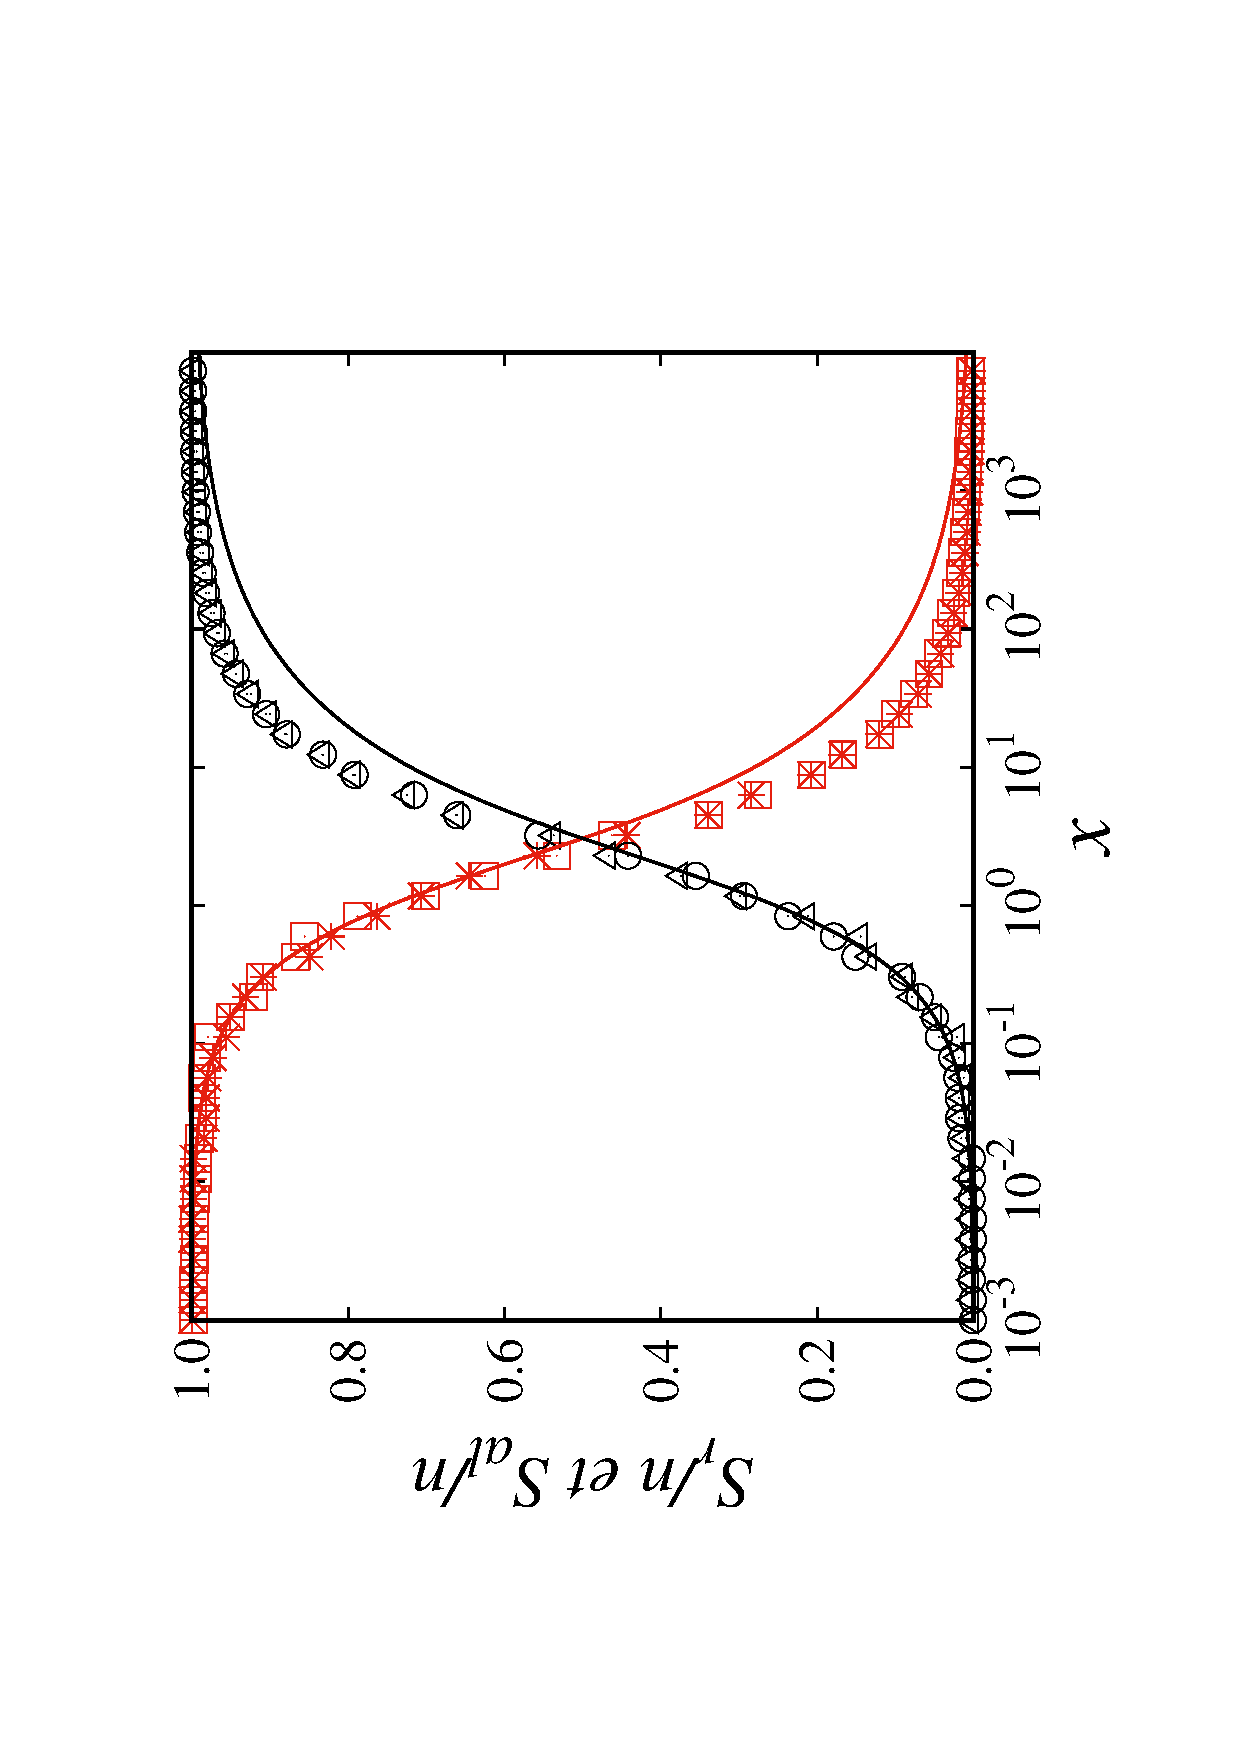
\includegraphics[scale=0.5,angle=-90]{./figures/fig-s}
	\caption{Fraction des nœuds aléatoires $S_{al}/n$ 
		(noir) et des nœuds réguliers $S_{r}/n$ (rouge)  en fonction de nombre des raccourcis $x$. Les lignes représentent les fonction $h(x)$  (noir) et $1-h(x)$ (rouge). Les symboles représentent les simulations numériques d'un réseau de taille $n=10^4$, avec
		$k=1$ (étoile et cercle) et $k=5$ (carré et triangle). Chaque simulation est moyennée à $200$ réalisations.}
	\label{S}
\end{figure}

Si on prend en considération la transformation de GR  qu'on a déjà utilisé dans nos calculs, les valeurs de $S'_{r}$ et $S'_{al}$ représentent en réalité le nombre des groupes $k$ de nœuds,
alors pour trouver le nombre réel des nœuds dans le réseau, il suffit de multiplier $S'_{r}$ et $S'_{al}$  par $k$
, car dans chaque groupe on a $k$ nœuds, d'où le nombre des nœuds réguliers est $S_r=n(1-h(kn\phi))$ et le nombre de nœuds 
aléatoires est $S_{al}=n h(kn\phi)$.
Sachant que la fonction $h(x)$ peut être considéré comme un paramètre d'ordre et selon son expression, on peut conclure qu'il n'y a pas une transition de phase dans ce modèle mais un phénomène de croisement qui commence depuis $x=0$. L'existence d'un tel paramètre d'ordre dans le modèle de NW est déjà une chose très importante, car il n'est pas toujours facile de le trouve, ainsi l'absence  d'un tel paramètre de ce modèle dans la littérature.  

\subsection{Plus court chemin}
On sait que l'expression du PCC s'écrit  $\ell=\sum_{i=1}^{\frac{\acute{n}}{2}}(i\cdot n_i)$, mais cette somme n'a pas une solution 
directe. Pour cette raison on va dissocier le PCC en deux types, exactement comme le cas des couches, d'où $\ell=\ell_{al}+\ell_r$, avec $\ell_r$ est le PCC du réseau régulier  et $\ell_{al}$ est le PCC du réseau aléatoire.\\
On commence par le PCC de réseau régulier $\ell_r$ qui s'écrit sous la forme 
\begin{equation}
\ell_r=\frac{S'_r}{\acute{n}}\frac{\int_1^{\frac{\acute{n}}{2}}i\cdot n_{i}^{r}di}{a_r},
\end{equation}
avec $a_r=\int_1^{\frac{\acute{n}}{2}}n_{i}^{r}di=S'_r$
est la constante de normalisation, d'où $\ell_r=\int_1^{\frac{\acute{n}}{2}}i\cdot\frac{n_{i}^{r}}{\acute{n}}di$.\\
De Eq.~\eqref{pr} et Eq.~\eqref{cr} on obtient
\begin{eqnarray}
\ell_r&=&\frac{1}{\acute{n}}\int^{\frac{\acute{n}}{2}}_1 2ie^{-4q\int_{j=1}^{i-1}(j-1)(q(\acute{n}-2j)+1)^{j-2}dj}di,\nonumber
\end{eqnarray}
en utilisant la m\^{e}me approximation précédente de l'Eq.~\eqref{sr} on obtient
\begin{eqnarray}
\ell_r &\approx&\frac{1}{\acute{n}}\int_1^{\frac{\acute{n}}{2}}2ie^{-2qi^2}di \\\nonumber
&\approx&\frac{1}{\acute{n}}\frac{e^{-2q}-e^{-\frac{q\acute{n}^2}{2}}}{2q}\\\nonumber
&\approx&\frac{1}{\acute{n}}\frac{1-e^{-\frac{q\acute{n}^2}{2}}}{2q} \quad \quad  \text{car:} \quad q\ll1 \\\nonumber
&\approx&\frac{\acute{n}}{4}\frac{1-e^{-\frac{q\acute{n}^2}{2}}}{\frac{q\acute{n}^2}{2}},\nonumber
\end{eqnarray}
sachant que $\frac{q\acute{n}^2}{2}=nk\phi=x$ et $\acute{n}=\frac{n}{k}$ alors $\ell_r$ peut s'écrire sous la forme universelle suivante
\begin{eqnarray}
\ell_r&\approx&\frac{n}{k}f_r(x) \quad \quad \textrm{avec} \quad f_r(x)=\frac{1-e^{-x}}{4x}.
\label{lr}
\end{eqnarray}

A fin de calculer $\ell_{al}$, nous utilisons la proposition que le PCC est la position de la couche maximale (voir Section.~\ref{pcc}). Dans notre cas ici c'est la position de la couche aléatoire maximale, de point de vue mathématique il suffit de résoudre $\frac{\partial n'_{al}(i)}{di}=0$. Soit $u(i)=4q(i-1)(q(\acute{n}-2i)+1)^{i-2}$, de l'Eq.~\eqref{pr} et Eq.~\eqref{pal} on obtient que $P_{al}(i)=u(i)e^{-\int_{j=1}^{i-1}u(j)dj}$. D'autre coté, il est évident que $\ell_{al}$ prédomine dans l'expression du PCC si $S_{al}\gg S_r$, alors la dimension de PCC devient négligeable devant la dimension de $\acute{n}$ car le nombre de raccourcis dans le réseau est important, d'où on peut prendre que $\acute{n}-2i\approx \acute{n}$, donc
$u(i)=4q(i-1)(q\acute{n}+1)^{i-2}$. Soit  $y=q\acute{n}$ le paramètre qui représente le degré moyen de raccourcis pour chaque nœud après la transformation de GR, car $q$ est la probabilité pour qu'un pair de nœuds se connecte et $\acute{n}$ est le nombre de nœuds.\\
 De l'Eq.~\eqref{cal} et $P_{al}(i)=u(i)e^{-\int_{j=1}^{i-1}u(j)dj}$  on obtient
\begin{eqnarray}
n'_{al}(i)=\acute{n}u(i)e^{-\int_{j=1}^{i-1}u(j)dj},
\end{eqnarray}
donc 
\begin{eqnarray}
\frac{\partial n'_{al}(i)}{\partial i}&=&\acute{n}\frac{\partial u(i)}{\partial i}e^{-\int_{j=1}^{i-1}u(j)dj}+\acute{n}u(i)\frac{\partial e^{-\int_{j=1}^{i-1}u(j)dj}}{\partial i}\\\nonumber
&=&\acute{n}\frac{\partial u(i)}{\partial i}e^{-\int_{j=1}^{i-1}u(j)dj}-\acute{n}u(i)^2e^{-\int_{j=1}^{i-1}u(j)dj},\nonumber
\end{eqnarray}
alors la solution de $\frac{\partial n'_{al}(i)}{\partial i}=0$ est la solution de l'équation suivante
\begin{equation}
\frac{\partial u(i)}{\partial i}-u(i)^2=0.
\label{28}
\end{equation}
On a $\frac{\partial u(i)}{\partial i}=u(i)\big[\frac{1}{i-1}+\ln(y+1)\big]$ et on sait que $ln(y+1)\gg\frac{1}{i-1}$, car $i$ reflet ici la valeur de PCC qui croit avec la taille 
du réseau $\acute{n}$, alors si $\acute{n}$ croit l'expression $\frac{1}{i-1}$ tend vers $0$, par contre $y=2k^2\phi$ ne dépend pas de la taille de réseau, d'où on peut négliger $\frac{1}{i-1}$ devant
$\ln(y+1)$ et  on obtient $\frac{\partial u(i)}{\partial i}=u(i)ln(y+1)$.\\
Alors l'Eq.~\eqref{28} devient
\begin{equation}
u(i)=\ln(y+1),
\label{29}
\end{equation}
si on remplace $u(i)$ par son expression $u(i)=4q(i-1)(q\acute{n}+1)^{i-2}=4q(i-1)(y+1)^{i-2}$, on va trouver la solution de l'Eq.~\eqref{29} qui nous 
donne la position de la couche-aléatoire maximal $i_{max}$ 
\begin{equation}
i_{max}=\frac{W\big(\frac{\ln(y+1)^2(y+1)}{4q}\big)}{\ln(y+1)}+1,
\end{equation}
avec $W(x)$ est la fonction de Lambert.\\
Alors selon notre proposition, la valeur de $\ell_{al}$ est $i_{max}$ multiplié par la fraction des nœuds aléatoires $\ell_{al}=i_{max}h(x)$, d'où 
\begin{equation}
\ell_{al}=(\frac{W\big(\frac{y+1)^2(y+1)}{4q}\big)}{\ln(y+1)}+1)h(x).
\label{lal}
\end{equation}
\begin{figure}[h!]
	\centering
	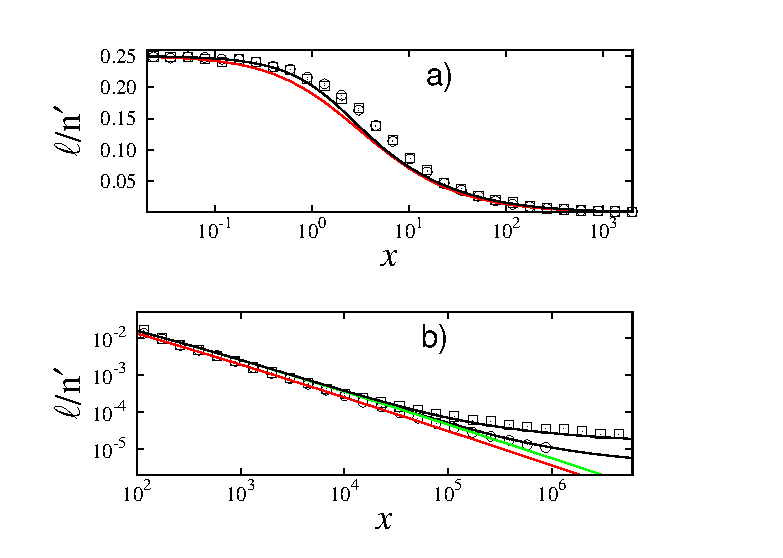
\includegraphics[scale=1.25,angle=0]{./figures/fig-kpn}
	\caption{L'expression universelle $f(x)=\ell/\acute{n}$ en fonction de $x$ pour un réseau de taille $n=10^6$. La formule de Newman et watts Eq.~\eqref{eq-ws} (ligne rouge), Eq.~\eqref{l2} (ligne vert), Eq.~\eqref{l} (ligne noir) et les simulations numériques pour $k=1$ (cercle) et $k=5$ (carré). L'échelle est linéaire-log dans \textbf{a)} et log-log dans \textbf{b)}. Chaque simulation est moyennée à $100$ réalisations.}
	\label{chemin}
\end{figure}

De l'Eq.~\eqref{lr} et Eq.~\eqref{lal} on obtient l'expression globale de PCC 
\begin{equation}
\ell=\bigg(\frac{W\big(\frac{\ln(y+1)^2(y+1)}{4q}\big)}{ln(y+1)}+1\bigg)h(x)+\acute{n}\frac{1-e^{-x}}{4x}
\label{l}
\end{equation}
pour trouver une expression universelle de $l$ en fonction du nombre des raccourcis $x$, il faut considérer que $y\ll 1$, d'où
\begin{eqnarray}
\ell=\acute{n}f(x) 
\label{l2}
\end{eqnarray}
avec $f(x)=\big(\frac{2W(\frac{x}{2})h(x)+1-e^{-x}}{4x}\big)$ est la nouvelle fonction universelle.\\
De la Fig.~\ref{chemin}, on voit que l'Eq.~\eqref{l} est en accord avec les simulations sauf dans l'intervalle
$1<x<20$  où il y a une certaine déviation, on explique cela par la proposition de l'existence des fluctuations élevé dans cette intervalle, car il est évident que lorsque les fluctuations devient importantes l'approximation du champs moyen n'est plus valable,  comme le cas usuel dans tous les systèmes physiques au voisinage des points critiques. On montre notre proposition par les simulations en utilisant le paramètre
d'ordre, $\frac{S_{al}}{n}$.
Soit $\sigma=\frac{\sqrt{\textless \frac{S_{al}}{n}^2\textgreater-\textless \frac{S_{al}}{n}\textgreater^2}}{\textless \frac{S_{al}}{n}\textgreater}$
les fluctuations de $\frac{S_{al}}{n}$ par rapport à sa taille,  en effet selon la Fig.~\ref{fluct} le maximum des fluctuations
est dans l'intervalle $1<x<20$ où l'Eq.~\eqref{l} montre une petite déviation.\\

\begin{figure}[h!]
	\centering
	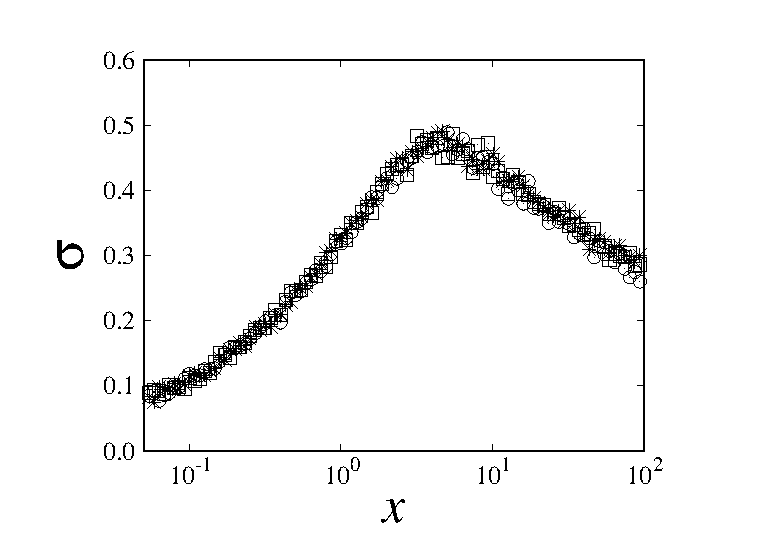
\includegraphics[scale=1,angle=0]{./figures/fig-f}
	\caption{Fluctuation $\sigma$ en fonction de $x$ d'un réseau de taille $n=10^4$  pour différents valeurs de $k$, $k=1$ (étoile), $k=2$ (carré) et $k=5$ (cercle), le nombre de réalisations est $1000$.}
	\label{fluct}
\end{figure}

\section{Émergence spectaculaire vers la propriété petit-monde}
\subsection{Échoué de l'ancien fonction universelle et la saturation des raccourcis}
Selon l'Eq.~\eqref{l}, l'expression universel $\ell=\acute{n}f(x)$
n'est plus valable si la condition $y\ll 1$ n'est pas vérifié, qu'on peut aussi montrer par les simulations numériques. Soit $\Delta$ l'écart de $\frac{\ell}{\acute{n}}$ en fonction
de $y$ entre un réseau de $n$, $k$ et $\phi$ donné et d'autres réseaux possédant des valeur aléatoires $n_{al}$, $k_{al}$ 
et $\phi_{al}$ sous la condition que $nk\phi=n_{al}k_{al}\phi_{al}$. L'expression de l'écart de $\frac{\ell}{\acute{n}}$  peut s'écrire  comme
\begin{equation}
\Delta=\frac{\frac{\ell}{\acute{n}}-\frac{\ell_{al}}{\acute{n_{al}}}}{\frac{\ell}{\acute{n}}+\frac{\ell_{al}}{\acute{n_{al}}}}.
\end{equation}

\begin{figure}[h!]
	\centering
	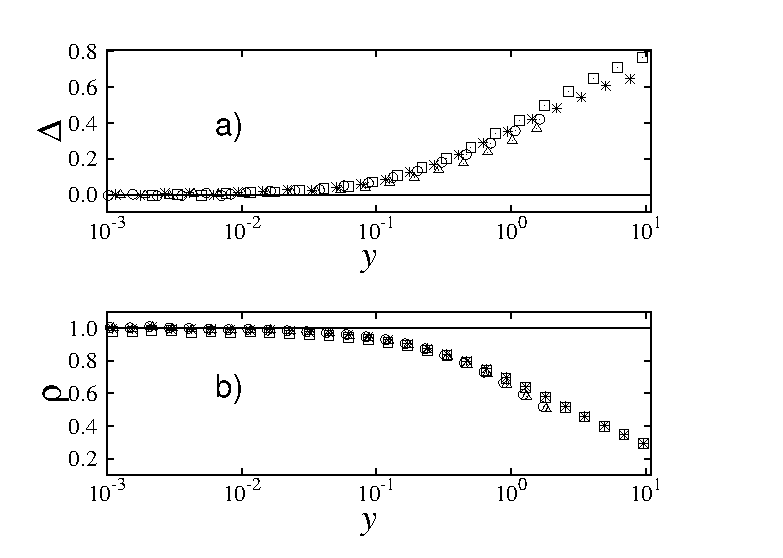
\includegraphics[scale=0.95,angle=0]{./figures/fig3-4}
	\caption{La valeur de $\Delta$ et $\rho$ en fonction de $y$ pour différent valeurs de $n$ et $k$:$n=10^{-3}$ et $k=1$ (triangle), $n=10^{-3}$ et	$k=4$ (carré),$n=10^{-4}$ et $k=1$ (cercle),$n=10^{-4}$ et $k=4$ (étoile). Dans   \textbf{a)} le nombre de réalisations pour chaque simulation est $1000$ et dans \textbf{b)} le nombre de réalisations pour chaque simulation est $5000$.}
	\label{def}
\end{figure}

De la Fig.~\ref{def}.(a) on observe une augmentation remarquable de $\Delta$ lorsque
$y$ n'est pas très inférieur à $1$, par intuition on peut expliquer ce phénomène par le début d'une saturation de raccourcis lorsque $y$ augmente, car après la saturation le réseau change son comportement devant les raccourcis ajoutés. Afin de montrer l'existence d'un changement de comportement vis-à-vis des raccourcis ajoutés, on va simuler numériquement le nombre de raccourcis existe dans le trajet de PCC entre deux nœuds choisi au hasard par rapport au nombre moyen des raccourcis dans le réseau, $\rho$, en fonction de $y$. En effet, selon les Fig.~\ref{def}.(a) et Fig.~\ref{def}.(b), on remarque une saturation de raccourcis qui varie d'une façon similaire avec $\Delta$ en fonction de $y$. Pour $y\ll1$ on voit que $\rho\approx1$, alors presque tous les raccourcis existent dans les trajets de PCC, c'est-à-dire l'impact des raccourcis sur le PCC est maximale, en revanche avec l'augmentation de $y$ le pourcentage des raccourcis existent dans les trajets diminue, c'est-à-dire l'impact des raccourcis sur le PCC se diminue.
On conclu que la saturation des raccourcis ajoutés explique bien la non validité de la fonction universelle $f(x)$ pour  $y\ll1$.\\
 
\subsection{La nouvelle fonction universelle }
La saturation des raccourcis peut signifier que le réseau commence à posséder la propriété petit-monde,
autrement dit le PCC devient de l'ordre de $\ln(n)$, pour confirmer cette proposition on réalise des simulations numériques et on  les compare avec notre équation. En effet, de la Fig.~\ref{fu} on voit que le rapport
$\frac{\ln(n)}{\ell}$ émerge et devient important d'une façon universelle en fonction du même paramètre $y$ avec lequel la saturation émerge. Alors une nouvelle équation universelle $g$ sous la forme $g(y)=\frac{\ln(n)}{\ell}$ apparaît.\\

Maintenant on essaye de formuler l'expression analytique de cette nouvelle équation universelle $g$, de l'Eq.~\eqref{l} on peut trouver facilement que dans la limite de grande taille de système on va obtenir que
\begin{eqnarray}
\frac{\ln(n)}{\ell}=\ln(y+1).
\label{kp1}
\end{eqnarray}

\begin{figure}[h!]
	\centering
	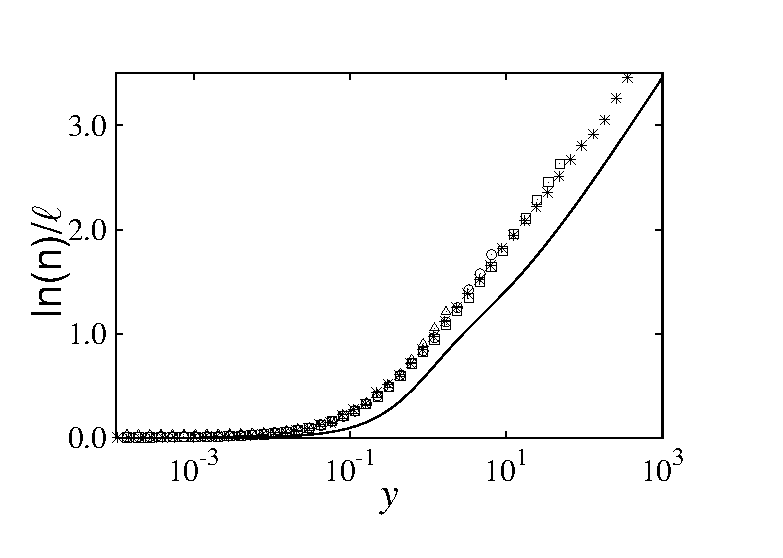
\includegraphics[scale=1,angle=0]{./figures/fig4-4}
	\caption{L'expression universelle de PCC en fonction de $y$, par Eq.~\eqref{kp2} (ligne continue) et par les simulations numériques pour différents valeurs de $n$ et $k$, $n=10^{-6}$ et $k=20$ (étoile), $n=10^{-5}$ et $k=5$ (carré), $n=10^{-4}$ et $k=2$ (cercle),$n=10^{-3}$ et $k=1$ (triangle), nombre de réalisations pour chaque simulations est $100$. En \textbf{a)} l' échelle est linéaire-log et en \textbf{b)} l'échelle est log-log.}
	\label{fu}
\end{figure}

Il est évident que l'Eq.~\eqref{kp1} n'est pas une expression exacte à cause de la transformation de GR que nous avons utilisé au début lorsque nous avons supposé que chaque $k$ voisins, on le dénommé ici \textsf{amas}, est comme  un seul nœud.\\
Sur le trajet de PCC entre deux amas quelconques dans le réseau on trouve des liens ordinaires et des raccourcis, dans le cas où il y a deux raccourcis successifs sur le trajet, c'est-à-dire on a deux raccourcis liant au m\^{e}me \textsf{amas}, la probabilité que les deux raccourcis liant au m\^{e}me nœuds dans cette amas est $\frac{1}{k}$ et la probabilité que les deux raccourcis ne lient pas au m\^{e}me nœud, c'est-à-dire on aura un lien en plus, est  $1-\frac{1}{k}$, autrement dit chaque fois on a deux raccourcis successifs il y a une probabilité de $1-\frac{1}{k}$ que le PCC augment par $1$.\\
D'autre part, le nombre des liens réguliers qui lient entre les \textsf{amas} est toujours
$\acute{n}$ et le nombre des raccourcis entre les \textsf{amas} est $\frac{q\acute{n}(\acute{n}-1)}{2}\approx\frac{q\acute{n}^2}{2}$, 
$q$ est la probabilité qu'un pair d'amas se connecte et $\frac{\acute{n}(\acute{n}-1)}{2}$ est le nombre des pairs possibles. Alors la fraction des raccourcis par rapport au nombre totale des liens est $\frac{q\acute{n}}{2+q\acute{n}}=\frac{y}{2+y}$, d'où la probabilité d'obtenir deux raccourcis liant au m\^{e}me \textsf{amas} dans le trajet entre deux nœuds quelconque est $(\frac{y}{2+y})^2$. Par conséquent la probabilité pour que la valeur de PCC sera doublé est $(\frac{y}{2+y})^2(1-\frac{1}{k})$, où $(\frac{y}{2+y})^2$ est la probabilité d'avoir deux 
raccourcis liant au m\^{e}me \textsf{amas}, et $(1-\frac{1}{k})$ est la probabilité que ces deux amas seront liant à deux nœuds différent. La probabilité que le PCC restera sans aucun changement est $(1-(\frac{y}{2+y})^2)+\frac{1}{k}(\frac{y}{2+y})^2$, le première terme représente la probabilité que deux raccourcis n'est pas liant au m\^{e}me \textsf{amas} et le deuxième représente la probabilité 
que deux raccourcis liant au m\^{e}me \textsf{amas} et au m\^{e}me nœud $\frac{1}{k}(\frac{y}{2+y})^2$, d'où l'Eq.~\eqref{kp1} devient
\begin{eqnarray}
\frac{\ln(n)}{l}=\frac{\ln(y+1)}{\frac{1}{k}(\frac{y}{2+y})^2+(1-(\frac{y}{2+y})^2)+2(1-\frac{1}{k})(\frac{y}{2+y})^2}
\end{eqnarray}
pour $k\gg1$ on obtient que
\begin{eqnarray}
\frac{\ln(n)}{\ell}=\frac{\ln(y+1)}{\big(1+(\frac{y}{2+y})^2\big)}
\label{kp2}
\end{eqnarray}
Cette fonction montre un certain écart par rapport aux résultats numériques, car dans notre calcul on n'a pas pris en compte tous les cas possibles des raccourcis entre les \textsf{amas} mais on a fait juste une approximation de champs moyen. Cependant notre
expression de $g(y)=\frac{\ln(y+1)}{\big(1+(\frac{y}{2+y})^2\big)}$ nous donne l'allure de la variation de la fonction universelle, qui varie d'une façon logarithmique.\\
Le fait qu'on a réussi à contrôler le nombre des raccourcis ajoutés pour atteindre la phase petit-monde dans le modèle de NW est une chose très importante et une contribution qui va enrichir tellement l'utilité de ce modèle. La difficulté qu'a empêché à répondre à ce problème  au cours des vingtième années précédente est de trouver le paramètre avec lequel on détermine le point où le réseau est saturé, alors par un raisonnement purement théorique on a trouvé que ce paramètre est $y$. 
\section{Conclusion}

En utilisant la transformation de GR sur le modèle NW, on a trouvé une expression analytique de PCC plus précise que l'ancien existé déjà dans la littérature, et à partir de cette nouvelle expression, on a conclu  que le paramètre $y$ est le variable avec lequel la propriété petit-monde émerge, le variable avec lequel on détermine  l'erreur et la validité de l'ancien fonction universelle $f(x)=\frac{\ell}{\acute{n}}$, le variable qui nous donne le degré de saturation de raccourcis, ainsi que le variable de la nouvelle fonction universelle $g(y)=\frac{\ln(n)}{\ell}$. On en déduit que l'émergence qui se passe en fonction de ce paramètre $y$ dans le modèle NW est une émergence spectaculaire.
\newcommand{\kma}{\textless k_a \textgreater}
\newcommand{\kmaa}{\textless k_a^2 \textgreater}
\chapter{Une nouvelle approche pour prédire les transitions de phases dans le phénomène de percolation}

La détermination du type de transition de phase dans le phénomène de percolation n'est pas encore devenue une science exacte, car on manque d'une règle qui  peut déterminer quelle transition sera de premier ou de second ordre. Cependant la détermination se fait au cours de la transition ou après, le but de ce chapitre est d'apporter une contribution concernant ce problème qui est un sujet très important dans le domaine de la physique fondamentale.   


\section{Introduction}
Le but ultime de l'étude des réseaux est de mieux comprendre le comportement des réseaux des systèmes. Par exemple, nous étudions la structure d'Internet pour mieux comprendre la manière avec laquelle le trafic Internet  circule, la façon du fonctionnement des protocoles de communication, ou comment organiser le réseau afin de le rendre plus performant. Nous étudions les réseaux biochimiques comme les réseaux métaboliques car nous espérons qu'ils permettent de    comprendre les processus chimiques complexes qui se déroulent dans la cellule, ou des outils algorithmiques pouvant nous aider à obtenir des informations biologiques de grands volumes de données générées par les techniques de laboratoire modernes\cite{Newman2010}. Nous étudions le réseau causal, qui représente la structure à grande échelle de l'espace-temps dans notre univers accéléré, pour comprendre pourquoi ce réseau est aussi un graphe de loi libre-échelle avec un regroupement fort \cite{Sungryong-Arjun2015}.\\
Notre but dans ce chapitre, à part le rappel théorique, est de mieux comprendre le comportement des transitions de phase dans les réseaux réels à partir
des approches dans le domaine des réseaux complexes. En bref, nous allons établir une formule pour prévoir le type de transition de phase au voisinage du point critique.

\section{Transition de phase}
Comme dans la fusion de la glace, ferro-magnétisme, la supraconductivité et le repliement des protéines, la nature contient quotidiennement des transitions de phase: processus dans lesquels les systèmes changent radicalement certaines propriétés physiques lorsqu'une variation minimale des variables se produisent.\\
En tenant compte de la grande présence des transitions de phase dans le monde réel, ce n'est pas étonnant que les physiciens aient commencé, depuis le tout début de la mécanique statistique, à découvrir des comportements universels et critiques (scaling à proximité des points de transition), ainsi que de faire un grand effort pour la classification des transitions de phase. La première tentative à fournir une classification a été réalisée par Ehrenfest [1], mais les schémas de classification les plus modernes regroupent les transitions de phase en deux grandes catégories : de premier et de second ordre.\\
En thermodynamique, les transitions de phase du premier ordre sont celles qui impliquent une chaleur latente, c'est-à-dire au cours d'elles le système absorbe ou libère une quantité typiquement élevée d'énergie par volume. Normalement, elles sont caractérisées (au point de transition) par "un régime en phase mixte", dans lequel certaines parties du système ont subi la transition et d'autres non, en présence ainsi d'une sorte de coexistence des phases des deux régimes. Les signes de telle transition sont: le comportement abrupt et discontinu du paramètre d'ordre à proximité du point de transition, ainsi que l'irréversibilité intrinsèque de la transition, avec la présence (dans la majorité des cas) de boucles hystérèses. En variante, les transitions de phase de second ordre (également appelées transitions de phase continues) sont réversibles et correspondent à des paramètres d'ordre présentant un comportement continu au voisinage du point critique.
Parmi les transitions du premier ordre nous citons la fusion de la glace, l'ébullition de l'eau, et les transitions de super-refroidissement et de surchauffe.Pour le second ordre nous avons la transition ferromagnétique, la supraconductivité et la transition super-fluide.
\section{Percolation}
La percolation est la transition vers la connectivité à grande échelle des réseaux suite à l'ajout progressif de liens, elle se produit au cours des processus de croissance et d'évolution dans une grande variété de systèmes naturels, technologiques et sociaux \cite{Strogatz2001,Newman-al2002,Song-al2006,Parshani-al2010,Parshani2-al2010,Ben-Avraham-Havlin2001,Saberi2015}. La percolation se produit aussi en physique dans les solides atomiques et moléculaires, ainsi que dans les réseaux sociaux, biologiques et artificiels \cite{Newman-al2002,Dorogovtsev-al2008,Rozenfeld-al2010}. Autrement dit, on peut dire qu'un système de percolation consiste à une grille, dans laquelle les nœuds ou les liens sont retirés avec une certaine probabilité $1-p$, ou on considère que les nœuds se lient avec une probabilité $p$ \cite{Bunde-Havlin1996,Stauffer-Aharony1994}, le système se déconnecte en petits groupes, c'est-à-dire qu'il devient impossible de passer d'une côté de la grille à l'autre en suivant les liens conducteurs, mais au-dessus de $p_c$, une grappe s'étend, semblable à la composante géante dans les graphiques aléatoires (voir Fig.~\ref{percolation}).

\begin{figure}[h!]
	\centering
	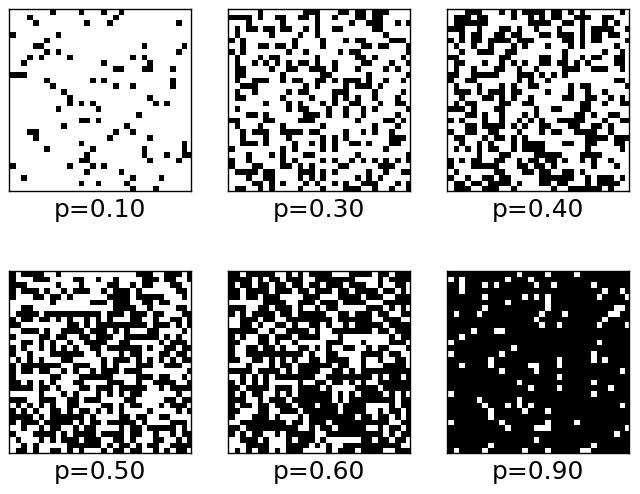
\includegraphics[scale=0.5]{./figures/percolation}
	\caption{Une démonstration de percolation sur une grille à deux dimensions pour différentes valeurs de $p$. Sous le seuil de percolation le système est composé de petites grappes, après un certain point critique $p_c$ une grappe étendue et occupe la grille.}
	\label{percolation}
\end{figure}
\section{Percolation explosive}
En percolation de liaison, on commence de $n$ nœuds non connectés. A chaque pas de temps, un lien est ajouté entre deux nœuds sélectionnés selon une règle donnée. Le nombre des liens ($E$) ajoutés au système à un certain pas de temps divisé par la taille du système est le paramètre de contrôle ($\km=\frac{2E}{n}$) qui décrit la transition de phase. En ce qui concerne le paramètre d'ordre, on peut prendre la fraction des nœuds appartenant à la composante géante du réseau (généralement noté $S(t)$). Au fur et à mesure que le temps augmente, le nombre de liens ajoutés dans le réseau augmente, dans la limite thermodynamique ($N\longrightarrow \infty$), $S(t)$ présente une transition de phase de zéro à $O(1)$ au voisinage d'un point critique ($\km_c$). La percolation classique est une transition de phase géométrique typique, qui a été largement étudiée depuis $1940$ dans de nombreux domaines, y compris les mathématiques, la physique statistique et l'ingénierie. De nombreux modèles de percolation, tels que la percolation d'invasion, de premier passage,  bootstrap et k-core. 
Tous ces modèles et beaucoup d'autres ont démontré que la transition de phases est étroitement liée à diverses applications, la turbulence, les modèles magnétiques, les colloïdes, la transition de Hall quantique spin, etc. Le lecteur est adressé aux revues récentes dans \cite{Boccaletti-al2016,Souza-Nagler2015,Araujo-al2014}, ses références contiennent un ensemble des principaux résultats et concepts de la percolation classique.\\

Pendant des décennies, la plupart des transitions de la percolation classique (ordinaire) semblent être de second ordre (continue) comme la percolation de liaison dans les réseaux ER, pour laquelle la taille de la composante géante augmente progressivement lorsque le paramètre de contrôle, $\km$, dépasse le seuil de percolation. Il convient toutefois de noter qu'il existe également de rares exemples de modèles de percolation présentant une transition de phase de premier ordre (discontinue), tels que la percolation bootstrap \cite{Adler1991}, k-core \cite{Dorogovtsev2-2006} et de brouillage \cite{Echenique-al2005}. Par l'observation que les règles de concurrence non locales ou globales lors des processus de fusion d'amas dans le réseau peuvent conduire à une percolation explosive PE, un certain nombre de ces processus, tels que ceux d'Achlioptas ont été étudiés \cite{Costa-al2010,Costa-al2015,Cho-Kahng2011}.
 \section{Percolation dans le réseau aléatoire d'Erd\H{o}s-Rényi}
 
 Un réseau aléatoire est créé en spécifiant que chaque paire de nœuds est connecté par un lien avec une probabilité uniforme $p$. Ce type de réseaux a été étudié d'un point de vue mathématique pure par Erd\H{o}s et Rényi \cite{Erdos-Renyi1959,Erdos-Renyi1960,Erdos-Renyi1961}, il est souvent désigné par son nom mathématique $G(n,m)$, avec $n$ est le nombre de nœuds et $m$ le nombre de liens. 
 Dans la cas où $n$ est très grand, bon nombre de propriétés de l'ensemble des réseaux aléatoires ont été exprimées analytiquement de façon parfaite et élégante.\\
 Les graphes aléatoires ER sont les mieux étudiés parmi les modèles de graphes, leurs propriétés structurelles varient en fonction de $p$ montrant notamment un changement radical à une probabilité critique $p_c=\frac{1}{n}$,
 correspondant à un degré moyen critique $\textless k \textgreater_c=1$. Erdös et Rényi ont prouvé que:\\
 \begin{itemize}
 	\item Si $p <p_c$, lorsque $n$ tend vers l'infini, le graphe n'a quasiment pas de composante de taille  
 	supérieure à $(ln(n))$.
 	\item Si $p=p_c$, la composante la plus importante a quasiment la taille de $n^{\frac{2}{3}}$.
 	\item Si $p> p_c$, le graphe a une composante de taille de l'ordre de $n$ et aucune autre composante n'a de taille supérieure à $(ln(n))$.
 \end{itemize}
 \begin{figure}[h!]
 	\centering
 	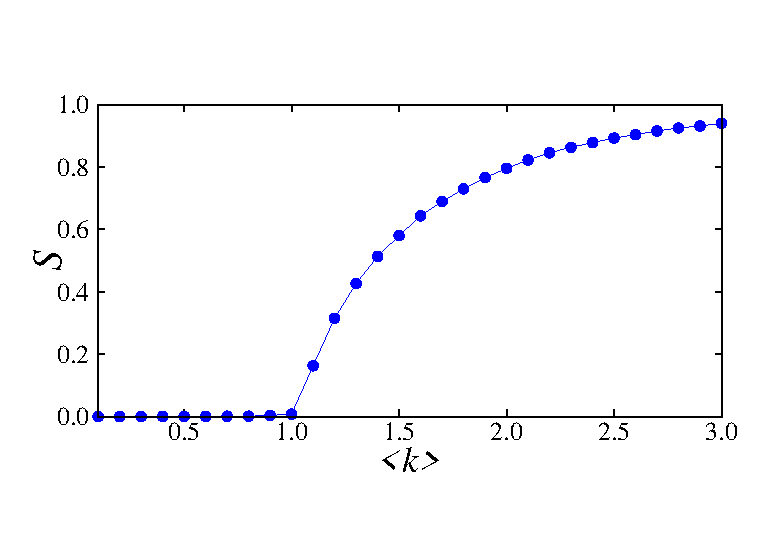
\includegraphics[width=12cm,height=9cm]{./figures/fig-ER-CG}
 	\caption{Les simulations numériques du seuil de percolation dans le modèle ER en fonction du degré moyen, pour un réseau de taille $n=10^5$. On observe que le point où la fraction de la composante géante, $S$, émerge est à $\textless k\textgreater=1$ .}
 	
 	\label{percolation-graph}
 \end{figure}
 
 La transition au $p_c$ présente les caractéristiques typiques d'une transition de phase de deuxième ordre. En particulier, si on considère la taille de la composante la plus importante comme paramètre d'ordre, la transition tombe dans la même classe d'universalité que celle des transitions de percolation de champ moyen (voir Fig.~\ref{percolation-graph}). Erdös et Rényi ont étudié la distribution des degrés minimum et maximum dans le graphe aléatoire, mais la distribution des degrés complet a été obtenue plus tard par Bollobás \cite{Bollobas1998}. La probabilité qu'un nœud possédant le degré  $k$ est la distribution binomiale:
 \begin{equation}
 P(k)=C^k_{n-1}p^k(1-p)^{n-1-k}
 \end{equation}
 Pour $n$ très grand, la répartition du degré est bien approchée par une distribution de Poisson:
 \begin{equation}
 P(k)=e^{-\textless k\textgreater}\dfrac{\textless k\textgreater^k}{k!}
 \label{ER}
 \end{equation}
 \begin{figure}[h!]
 	\centering
 	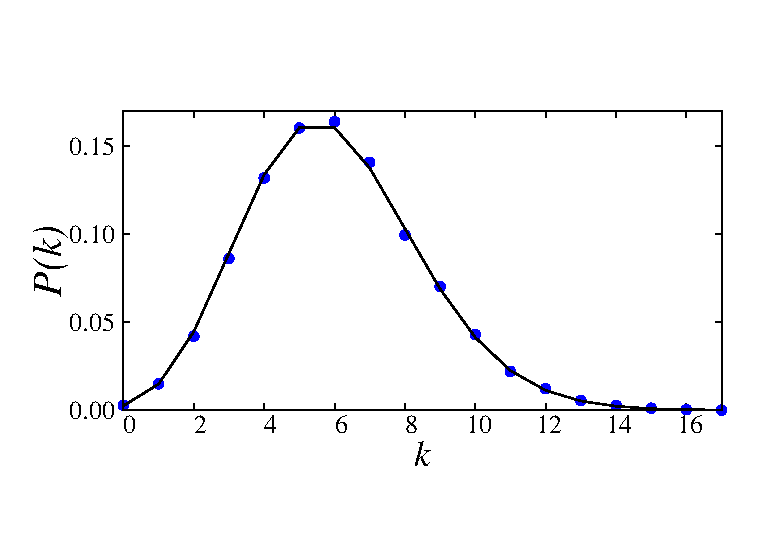
\includegraphics[scale=1]{./figures/fig-ER-dist}
 	\caption{Illustration de la distribution des degrés d'un réseau aléatoire ER de degré moyen égale $6$, les cercles représentent les simulations numériques et la ligne noire représente Eq.~\eqref{ER}.}
 	
 	\label{ER-distribution}
 \end{figure} 
 
 Le coefficient de regroupement, $C$, est une quantité très simple à calculer pour le graphe aléatoire de Poisson, rappelons qu'il est défini comme la probabilité que deux voisins d'un nœud du réseau soient également voisins les uns des autres. Dans un graphe aléatoire, la probabilité que les deux nœuds soient voisins est égale à $p=\frac{\textless k\textgreater}{(n - 1)}$. Par conséquent:
 
 \begin{equation}
 C=\dfrac{\textless k\textgreater}{(n - 1)}
 \end{equation}
 
 Cette valeur de Clustering qui tend vers $0$ quand $n$ tend vers l'infini est l'un des nombreux aspects dans lesquels le graphe aléatoire diffère fortement de la plupart des réseaux réels, dont beaucoup ont des coefficients de regroupement assez élevés.

\subsection{Percolation explosive dans le processus d'Achlioptas}

L'idée principale du processus Achlioptas (PA) \cite{Achlioptas-al2009} est de modifier la règle pour générer des graphes ER. Au lieu d'ajouter des liens aléatoires, dans le processus Achlioptas on choisit deux liens au hasard puis on utilise une règle pour sélectionner l'un ou l'autre. Le lien sélectionné sera ajouté au graphe alors que l'autre lien sera rejeté. Considérons la Fig.~\ref{achlioptas} (adapté de \cite{Achlioptas-al2009}): (\textbf{A}) l'évolution du réseau  selon le modèle ER, à chaque étape deux nœuds sont choisis au hasard et reliés par un lien (représenté par la ligne pointillée). Dans cet exemple, deux composantes de taille $7$ et $2$ sont fusionnées. (\textbf{B}) Deux liens aléatoires $\{e_1,e_2\}$ sont sélectionnés à chaque étape mais un seul sera ajouté au réseau suivant une règle de sélection, tandis que l'autre sera abandonné.
Soumettant à la règle de produit (RP), le lien sélectionné est celui qui minimise le produit des tailles des composantes qui sont fusionnées. Pour cet exemple, $e_1$ (avec le produit $2\times7=14$) sera choisi et $e_2$ rejeté (parce que $4\times4=16$). En revanche, la règle avec laquelle on sélectionne le lien minimisant la somme des tailles des composantes choisi $e_2$ au lieu de $e_1$. (\textbf{C}) Évolution de fraction de la composante géante  $\frac{C}{n}$ pour: ER, BF (une règle de taille bornée, voir \cite{Bohman-Frieze2001}), et RP. Le réseau étudie est de taille $n=512000$.
\begin{figure}[h!]
	\centering
	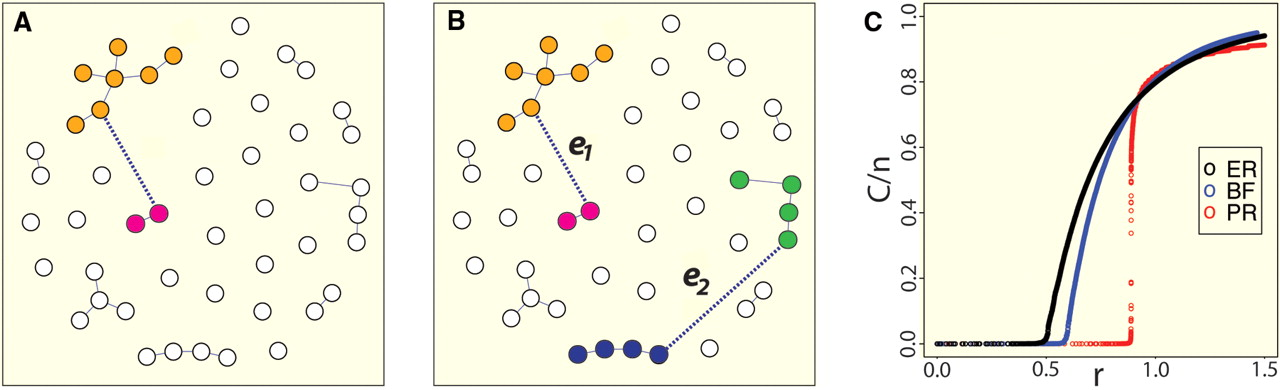
\includegraphics[scale=0.35]{./figures/achlioptas3}
	\caption{Comparaison entre la percolation aléatoire et PA. (\textbf{A}) Percolation ER classique, où les liens sont ajoutés au hasard dans le réseau. (\textbf{B}) Percolation PA, où à chaque étape deux liens sont en compétition pour être établis. (\textbf{C}) Paramètre d'ordre: la taille relative de la composante géante par rapport au nombre des liens ajoutés normalisés par la taille du système.}
	\label{achlioptas}
\end{figure}

Achlioptas s'est demandé s'il était possible de déplacer le point critique de cette transition de phase suivant une règle de sélection appropriée. Une règle qui peut naturellement être imaginée c'est la règle du produit: Parmi les liens donnés, choisir celui qui minimise le produit des tailles des composantes contenant les quatre extrémités de $\{e_1,e_2\}$. Cette règle a été suggérée dans \cite{Bollobas-1984} comme la plus susceptible de retarder le point critique. Une autre règle est la règle de somme, où la taille de la nouvelle composante formée est minimisée. La Fig.~\ref{achlioptas}.(c) est  suffisante pour motiver l'idée pour que la transition de percolation RP soit discontinue. Achlioptas et al. ont utilisé une méthode intéressante pour vérifier que la transition est bien discontinue. Ils mesurent numériquement le pas de temps $t_0$ auquel la taille de la composante géante $(C)$ devient plus grande que $n^{\frac{1}{2}}$ et $t_1$ où $C$ devient plus grand que $\frac{1}{2}\times n$. Un pas de temps correspond à une valeur de $r$ où $r=\frac{E}{n}=\frac{t}{n}$ (puisque le nombre de liens à l'instant $t$ est $E$). Pour le modèle ER et d'autres transitions de percolation continues, on trouve que $\Delta\equiv t_1-t_0$ est extensive, c'est-à-dire il évolue avec $n$. En outre, pour le modèle RP, ils ont trouvé que $\Delta\sim n^{\frac{2}{3}}$. Puisque $\Delta$ est sous-linéaire en $n$, c'est un argument numérique qui montre que dans la limite thermodynamique $n\rightarrow \infty$ la transition de percolation est en effet discontinue.

Cependant, cette conjecture a été rapidement et  rigoureusement désapprouvée par Riordan et Warnke \cite{Riordan-Warnke2011,Riordan-Warnke2012}, en montrant qu'il ne s'agit pas d'une transition discontinue  mais continue. En effet, leur argument montre des transitions de phase continues pour une classe encore plus grande de processus PA \cite{Riordan-Warnke2012}. Leurs résultats indiquent que la continuité de la transition de phase est une caractéristique assez robuste et donc tous les processus Achlioptas ont une transition de phase continue. En revanche, Nagler et ses collègues \cite{Nagler-al2012} ont montré qu'il est également vrai que certains processus de percolation basés sur le choix d'un nombre fixe de sommets aléatoires sont discontinus, et ils ont résolu ce paradoxe apparent. En identifiant et analysant un processus  continu dans le sens défini par Riordan et Warnke \cite{Riordan-Warnke2012} mais qui présente encore un nombre infini de sauts discontinus dans un voisinage arbitraire du point de transition: un escalier du Diable. Ils ont démontré analytiquement que la continuité à la première transition de connectivité et la discontinuité du processus de percolation sont compatibles pour certains systèmes de percolations compétitifs.\\

La percolation explosive est un problème scientifique très intéressant dans des champs de recherche plus larges que la percolation. Il détient un potentiel considérable pour faire progresser notre connaissance des transitions de phase et des phénomènes critiques. Le fait qu'une légère modification des règles de sélection classiques puisse modifier de manière significative la classe d'universalité de la transition de phase sous-jacente est impressionnant. De plus, il semble que dans des cas extrêmes, l'ordre de transition lui-même puisse également changer.

\subsection{Percolation explosive dans d'autres modèles}
Au-delà de la percolation ordinaire, de nombreux autres modèles ont été développés en se basant sur diverses contraintes concernant l'occupation des liens afin de produire PE. Dans ce qui suit, nous examinons brièvement certains de ces modèles selon la référence \cite{Boccaletti-al2016}: 
\subsubsection{Les modèles de probabilité}
Ce modèle consiste à donner pour tout amas $i$ un poids $s_i$, pour chaque pas de temps un lien entre une paire d'amas $ij$ est occupé par une probabilité proportionnelle à $(s_is_j)^{\alpha}$. La somme  de tous les poids est déterminée comme une constante de normalisation: $w=\sum_i\sum_j(s_is_j)^{\alpha}$, alors la probabilité pour que l'amas $i$ soit lié à un autre amas $j$ est $\frac{(s_is_j)^{\alpha}}{w}$ \cite{Cho-al2010}.\\ Un autre exemple de ces modèles est le modèle hamiltonien de la référence \cite{Moreira-al2010}, on commence par un réseau de $n$ nœuds sans aucun lien, de sorte que chaque nœud appartient initialement à un amas différent. Tout d'abord, un hamiltonien $H$ simple est défini en fonction des tailles des grappes et du nombre de liens ajoutés à ces grappes. Ensuite, un nouveau lien $e$ entre toute paire de nœuds non encore connectés est ajouté, avec une probabilité proportionnelle à $e^{(-\beta\Delta H_e)}$, où $\Delta H_e$ est le changement d'énergie après l'ajout d'un lien.

\subsubsection{Les modèles Hybrides}
Dans les modèles hybrides la composition des arêtes suit à la fois des règles de percolation ordinaire et des règles concurrentielles: à chaque pas de temps, un lien peut être choisi aléatoirement avec probabilité $p$, alors qu'il peut aussi être choisi suivant une règle concurrentielle donnée par la probabilité $1-p$. Par exemple, dans \cite{Bastas-al2014} RP est utilisée, dans la référence \cite{Cao-Schwarz2012} un mélange de $k=2$ et $k=3$-core sur le réseau aléatoire, un mélange de $k=3$-core et des modèles de percolation de brouillage dans le réseau 2D sont étudiés. Les modèles hybrides ont été analysés dans des réseaux 2D \cite{Cao-Schwarz2012,Bastas-al2014} et des réseaux ER  \cite{Cao-Schwarz2012,Bastas-al2014,Fan-al2012}.
\subsubsection{Les modèles bootstrap}
Dans le cadre du PE, certains modèles bootstrap ont été proposés \cite{Baxter-al2010}. Le processus standard de percolation bootstrap sur un treillis en supposant que les sites sont actifs ou inactifs et que l'état d'un site dépend de ses voisins. Initialement, chaque site est actif avec une probabilité $p$, et inactif avec probabilité $1-p$. Chaque site activé reste dans son état, alors que chaque site inactif peut devenir actif (et rester actif pour toujours) si ses $k$ voisins les plus proches sont actifs (avec $k=2,3,\ldots$). La procédure est poursuivie jusqu'à ce que le système atteint la configuration stable . Dans l'état final du processus, on s'intéresse à savoir s'il existe  une composante géante occupée par des sites actifs. La percolation bootstrap peut montrer des transitions continues ou discontinues, selon le type du réseau et sa dimension.
\begin{sloppypar}
	
\section{Percolation au voisinage du point critique: approche théorique et simulation}
\end{sloppypar}
\subsection{Introduction}
La détermination du type de la transition de phase dans le phénomène de percolation n'est pas encore devenue une science exacte, c'est-à-dire, il manque une règle avec laquelle on peut déterminer qu'une telle transition est de premier ou de second ordre indépendamment des mécanismes locaux d'évolution du système ou modèle étudié, même si la percolation est l'un des modèles les plus simples et les plus anciens dans la physique statistique. Cependant pour quelques modèles spécifiques, par exemple dans \cite{Ziff-al1983}, une approche de l'équation du taux a été utilisée pour déterminer le type de transition de phase de la percolation, comme exemple dans l'évolution des réseaux ER, l'équation différentielle est écrite dans la limite thermodynamique par:
\begin{equation}
\frac{\partial n_s(t)}{\partial t}=\sum_{i+j=s}\frac{k_in_i}{c(t)}\frac{k_jn_j}{c(t)}-2\frac{k_sn_s}{c(t)},
\label{ED-5}
\end{equation}
où $c(t)=\sum_{s}k_sn_s$ est la constante de normalisation, $\frac{k_in_i}{c(t)}\frac{k_jn_j}{c(t)}$ est la probabilité qu'une amas de taille $i$ et de poids $k_i$ sera connecte à un amas de taille $j$ et de poids $k_j$ et $2\frac{k_sn_s}{c(t)}$ est la probabilité qu'un amas de taille $s$ et de poids $k_s$ sera connecté à n'import quel amas dans le réseau.\\
Dans \cite{Cho-al2010,Cho2-Kahng2011} les auteurs ont généralisé l'Eq.~\eqref{ED-5} en prenant $k_i=i^{\omega}$, le cas $\omega=1$ est exactement le cas ER. En utilisant la technique de fonction génératrice, ils ont trouvé l'expression de distribution d'amas au point critique, $n_s(t_c)\sim s^{-\gamma}$, où $\gamma$ est déterminer comme:
\begin{align}
\gamma &=
\begin{cases}
1+2\omega & \text{si}\ 0<\omega<\frac{1}{2} \\
 \frac{1}{2}+\omega& \text{si}\ \frac{1}{2}<\omega<1.
\end{cases}
\label{gama}
\end{align}

En se basant sur des simulations numériques, on a trouvé que pour $\frac{1}{2}<\omega<1$ la transition de phase est continue et pour $0<\omega<\frac{1}{2}$ la transition est discontinue. On peut déterminer par simulation le type de transition de percolation dans ce modèle en mesurant l'exposant $\omega$ en termes de processus d'agrégation de cluster. En 1983, un modèle unidimensionnel de percolation a été introduit \cite{Schulman1983} dans lequel les sites $i$ et $j$ sont reliés par la probabilité $p_{ij}=\frac{p}{\mid i-j\mid^s}$, où $p$ est un paramètre défini dans l'intervalle $0\leq p\leq1$, et $s$ est aussi un paramètre. Dans la référence \cite{Aizenman-Newman1986} les auteurs ont prouvé que la transition est discontinue pour $1<s\leq2$ et ils ont fait d'autres progrès notables associés à la percolation à longue distance, pour plus de détails voir \cite{Lee-al2016}.\\
Dans ces modèles la caractérisation des transitions de phase dépend de certains paramètres intrinsèques  et n'est pas une caractérisation générale qu'on peut appliquer à tous les différents modèles de percolation. La question qui se pose: Est-il possible d'unifier la loi qu'on peut utiliser pour déterminer le type de la transition ? Pour répondre à cette question, il faut d'abord trouver les paramètres ou les grandeurs avec lesquelles on va établir cette unification.\\
Pour cette raison, on propose une méthode qui peut prédire le type de la transition de phase au voisinage du point critique en admettant que la distribution d'amas dans le réseau au voisinage du point critique suit toujours une loi de puissance, on définit deux paramètres: le premier est l'exposant $\gamma$ de la distribution d'amas au voisinage du point critique, $P(s)=cs^{-\gamma}$, avec $c$ est la constante de normalisation. Le deuxième paramètre est $\gamma'$ qui dépend de la façon de choisir les amas, plus précisément il dépend des corrélations existantes dans le réseau, car dans les réseaux corrélés la probabilité de choisir une amas de taille $s$ est différente de sa distribution réelle. Par exemple, dans la Fig.~\ref{gama-5} on observe que dans le cas d'un processus Achlioptas, l'exposant de la distribution d'amas avec laquelle les amas sont choisies, $\gamma'$, est différente à la distribution d'amas réelle $\gamma=2.5$, par contre dans le cas aléatoire les distributions restent exactement les mêmes, $\gamma'=\gamma=2.5$. Autrement dit, dans les réseaux non-corrélés la probabilité de choisir un amas est exactement liée à sa distribution, ce qui n'est pas le cas avec l'existence des corrélations. D'où on définit la distribution dont les amas sont choisies par $P(s)'=c's^{-\gamma'}$, avec $c'$ est la constante de normalisation.
% En outre, on peut dire que la valeur moyenne des amas choisissent par les liens ajoutés est différents au valeur moyenne des amas dans le réseau, cette  différence de valeur moyenne est similaire au celle dans \cite{Lachgar-Achahbar2016} où les auteurs, en basant sur le degré moyen de nœuds choisi à chaque instant, ont comparé le modèle de BA avec sa complément, le degré moyen utilisé est différent au degré moyen des nœuds usuel. 
 \begin{figure}[h!]
 	\centering
 	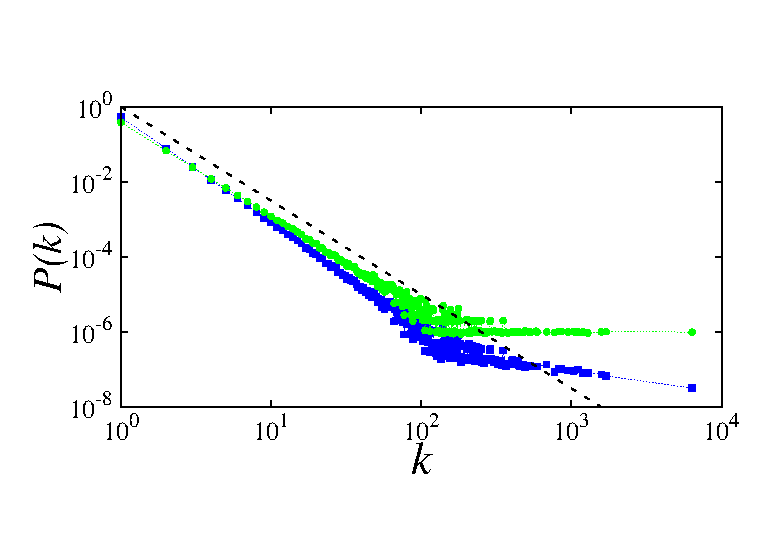
\includegraphics[scale=1.2]{./figures/fig-gama}
 	\caption{La distribution d'amas selon deux méthodes différentes pour choisir les liens dans le même réseau, où l'exposant de la distribution d'amas dans le réseau est $\gamma=2.5$, la première méthode est aléatoire comme le processus ER (cercles verts), la deuxièmes est par le processus Achlioptas \cite{Achlioptas-al2009} (carrés bleus). La ligne pointillée a pour but de montrer  l'exposant  $\gamma=2.5$. La taille du réseau est $n=10^6$, chaque simulation a une moyenne de $n$ réalisations. }
 	\label{gama-5}
 \end{figure}
 
\subsection{Approche théorique}
\subsubsection{Composante géante:}
Dans cette partie nous allons élaborer une expression de la composante géante, beaucoup plus générale que celle de ER, au voisinage du point critique en fonction de deux paramètres $\gamma$ et $\gamma'$.
Nous supposons que le point critique est notre temps initial, puis nous ajouterons des liens au réseau.
Pour qu'un amas de taille $i$ n'appartienne pas à la composante géante, il ne doit pas être connecté à la composante géante via un autre amas de taille $j$. Cela signifie que: (a) l'amas de taille $i$ n'est pas connecté à l'amas de taille $j$ par un lien, ou (b) l'amas  de taille $i$ est connecté à l'amas de taille $j$, mais l'amas de taille $j$ n'est pas elle-même membre de la composante géante.\\
Soit $p=\frac{\km}{n-1}$ la probabilité que deux nœuds se connectent, où 
$\km=\frac{2\times\text{(nombre de liens ajoutés)}}{\text{n}}$ est la densité des liens ajoutés par rapport à la taille du réseau.
La probabilité du résultat (a) est $(1-p)^{ij}$, et la probabilité du résultat (b) est $(1-(1-p)^{ij})u$, où $u$ est la probabilité qu'un nœud n'appartienne pas à la composante géante. D'où la probabilité qu'un amas de taille $i$ n'appartienne pas à la composante géante à travers n'importe quel amas de taille $j$  dans le réseaux est
\begin{eqnarray}
q_{ij}&=&[(1-p)^{ij}+(1-(1-p)^{ij})u]^{n_aP(j)'}\nonumber\\
&\approx&[1-ijp(1-u)]^{n_aP(j)'}\nonumber\\
&\approx&e^{-ijp(1-u)n_aP(j)'},
\end{eqnarray}
 avec $P(j)'=c'j^{-\gamma'}$ est la probabilité de choisir un amas de taille $j$ et $n_a$ est le nombre des amas.
D'où la probabilité qu'un amas de taille $i$ n'appartienne pas à la composante géante à travers n'importe quel amas est
\begin{eqnarray}
\pi_{i}&=&\prod_{j=1}^{K}q_{ij}\nonumber\\
       &=&e^{-ipn_a(1-u)\sum_{j=1}^{K}jP(j)'},
\end{eqnarray}
où $K=n_a^{\frac{1}{\gamma'-1}}$ est l'amas maximal au voisinage du point critique $(\km_c)$.\\ D'où $\sum_{j=1}^{K}jP(j)'=\kma'$ est le degré moyen avec lequel les amas sont choisis au réseau, ainsi que $\kma$ est la valeur moyenne des amas, alors $n=n_a\kma$, et on sait que $p=\frac{\km}{n-1}$, on peut écrire
\begin{eqnarray}
\pi_{i}=e^{\frac{-i(1-u)\km\kma'}{\kma}}.
\label{pi}
\end{eqnarray}
La fraction des amas de taille $i$ qui n'appartiennent pas à la composante géante par rapport à la taille de réseau $n$ est 
\begin{eqnarray}
u_{i}=\frac{n_aiP(i)\pi_i}{n},
\label{ui}
\end{eqnarray}
d'où la fraction des nœuds qui  n'appartiennent pas  à la composante géante est
\begin{eqnarray}
u=\sum_{i=1}^K u_i.
\end{eqnarray}
Alors la fraction des nœuds qui appartiennent à la composante géante est 
\begin{eqnarray}
S=1-u=1-\sum_{i=1}^K u_i.
\end{eqnarray}
De Eq.~\eqref{pi}, Eq.~\eqref{ui} et sachant que $n=n_a\kma$ et $S=1-u$ on obtient
\begin{eqnarray}
S&=&1-\frac{1}{\kma}\sum_{i=1}^KiP(i)e^{\frac{-iS\km\kma'}{\kma}}\nonumber \\
&=& 1-\frac{1}{\kma}\int_{i=1}^KiP(i)e^{\frac{-iS\km\kma'}{\kma}}di.
\label{s}
\end{eqnarray}
 Cette formule ci-dessus est une expression beaucoup plus générale que celle de ER \cite{Erdos-Renyi1959}. En effet, dans le cas où on ajoute aléatoirement des liens sans corrélations ,$\gamma=\gamma'$, et lorsqu'au temps initial tout amas a la taille $1$, on va trouver exactement l'expression de ER, $S=1-e^{-S\km}$.
  \begin{figure}[h!]
  	\centering
  	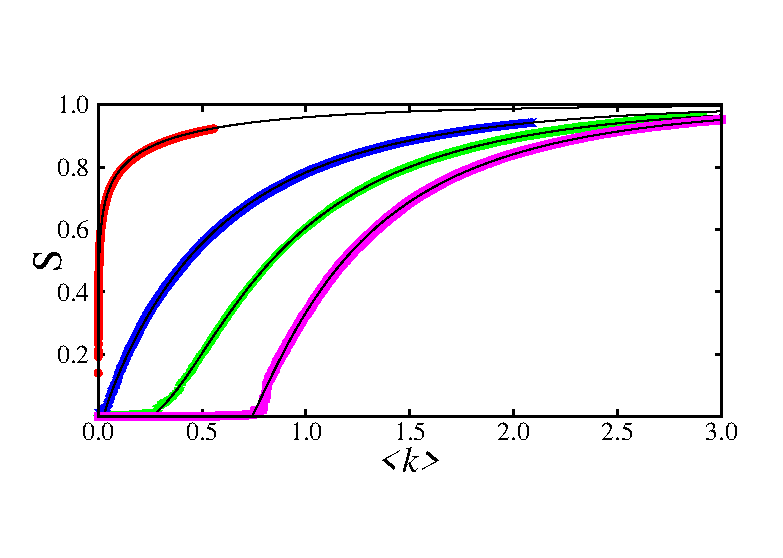
\includegraphics[scale=1.2]{./figures/fig-CG}
  	\caption{Fraction de la composante géante $S$ en fonction de la densité des liens $\km$ pour différentes valeurs de $\gamma$, les couleurs de gauche à droite représentent  respectivement les simulations numériques pour $\gamma=2,2.5,3,4$, les lignes noire représentent la solution numérique de l'Eq.~\eqref{s}. Le nombre des nœuds est $n=10^5$.}
  	\label{CG}
  \end{figure}
 
 \subsubsection{Détermination du point critique:}
 A partir de Eq.~\eqref{s} et en se basant sur une solution graphique citée dans \cite{Newman2010-403} on peut obtenir facilement le point critique $\km_c$ où la composante géante apparaît, cette méthode s'appuie sur la condition que le point critique $\km$ justifie  
 \begin{equation}
 \frac{\partial (1-\frac{1}{\kma}\sum_{i=1}^KiP(i)e^{\frac{-iS\km\kma'}{\kma}})}{\partial S}\Big)_{S=0}=1,
 \end{equation}
 la solution de cette équation ci-dessus nous donne l'expression suivante
 \begin{equation}
\km_c=\frac{\kma^2}{\kmaa\kma'},
 \end{equation}
 dans le cas où il n'y a pas de corrélations $\gamma=\gamma'$, c'est-à-dire $\kma=\kma'$, on obtient 
  \begin{equation}
  \km_c=\frac{\kma}{\kmaa}=\frac{1}{\kappa_a},
  \label{kc}
  \end{equation}
   cette expression est beaucoup plus exacte de celle donnée par \cite{Cho-al2010}, où les auteurs ont trouvé que $\km_c=\frac{1}{\kmaa}$, mais en se basant sur les simulations numériques (voir Fig.~\ref{PC} ) il est claire que notre formule est plus exacte.\\
\begin{figure}[h!]
	\centering
	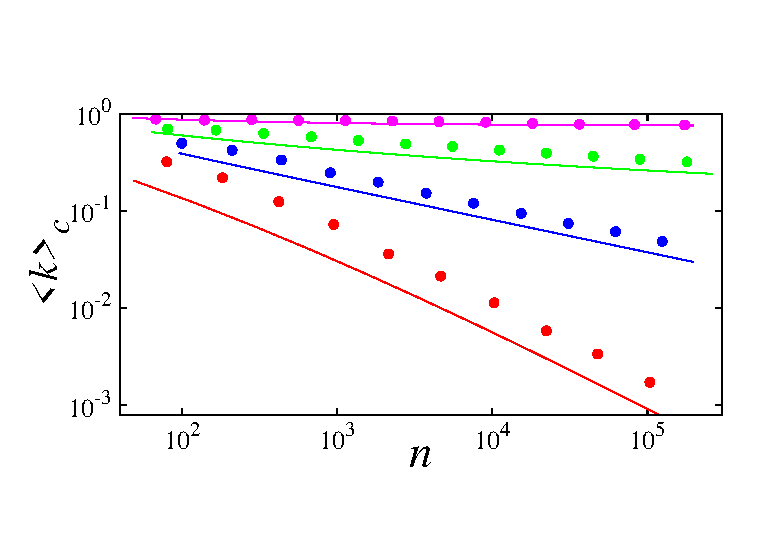
\includegraphics[scale=1.2]{./figures/fig-PC}
	\caption{Estimation de point critique par les simulations numériques (cercles) et par Eq.~\eqref{kc} (ligne). Les valeurs de $\gamma$ de haut en bas sont respectivement $4,3,2.5,2$. Chaque simulation est moyennée à $500$ réalisations. }
	\label{PC}
\end{figure}

Il convient de mentionner que la détermination du point critique par les simulations n'est pas une opération facile, il est assez compliqué et délicat de la trouver avec une grande précision. Dans nos simulations présentées dans la Fig.~\ref{PC}, nous avons estimé le point critique par la détermination d'un point où la valeur moyenne des petits amas dans le réseau est maximale,  cependant cette estimation est devenue plus précise avec l'augmentation du nombre des nœuds du réseau, car les effets d'échelle diminuent avec la taille. Alors que l'expression théorique semble exacte, le problème reste la détermination du point critique par les simulations numériques. 
 
 
  \subsubsection{Détermination du type de transition de phase:}
 Pour déterminer le type de la transition de phase on va essayer de calculer la valeur de $\km$ pour que $S$ atteigne une valeur à l'échelle macroscopique, $O(1)$, (par exemple $S=\frac{1}{4}$), si $\km$ tend vers zéro on dit que la transition est de premier ordre sinon on dit qu'elle est de second ordre.\\
 A partir de Eq.~\eqref{s} et sachant que $P(i)=ci^{\gamma}$, on obtient
 \begin{equation}
 S=1-\frac{c}{\kma}\int_{i=1}^Ki^{1-\gamma}e^{\frac{-iS\km\kma'}{\kma}}di
 \label{s2},
 \end{equation}
 l'intégrale dans cette expression n'a pas de solution explicite connu, alors il est impossible d'extraire la valeur de $\km$ en fonction de $S$,  pour cette raison on propose une autre approche, on va construire la composante géante par la manière la plus rapide possible, puis on déduit le type de la transition de phase selon $\gamma$ et $\gamma'$.\\
 Pour chaque nouveau lien, on lie les deux amas les plus grands dans le réseau\footnote{Cette approche est valable sauf au voisinage du point critique lorsque la distribution d'amas suit une loi de puissance, car lorsqu'on commence à ajouter les liens par cette méthode loin du point critique, cela peut ralentir  la transition au point critique au lieu de l'accélérer.}, mathématiquement on traduit cela par l'expression suivante 
  \begin{equation}
  S=\sum_{i=1}^tk(t)=\int_{1}^{t}k(i)di,
  \label{s3}
  \end{equation}
  où $t$ représente le temps et également le nombre des liens ajoutés, et $k(t)$ est $t^{\text{ème}}$ degré maximal, avec $k(1)=K$.\\
  $k(t)$ peut être calculé par l'expression suivante
  \begin{equation}
  \sum_{i=k(t)}^Kn_aP(i)=\int_{i=k(t)}^Kn_aP(i)di=t,
  \end{equation}
 d'où on obtient
   \begin{eqnarray}
   k(t)&=&\Big(K^{1-\gamma}+\frac{(\gamma-1)t}{cn_a}\Big)^{\frac{1}{1-\gamma}}\nonumber\\
     &=& \Big(\frac{t+1}{n_a}\Big)^{\frac{1}{1-\gamma}} \quad \quad  \text{car:} \quad c=\gamma-1 \quad \text{et} \quad K=n_a^{\frac{1}{\gamma-1}} \nonumber\\
     &=& \Big(\frac{t}{n_a}\Big)^{\frac{1}{1-\gamma}}
     \quad \quad  \text{car:} \quad t+1\approx t,
     \label{kt}
   \end{eqnarray}
 de Eq.~\eqref{s3} et Eq.~\eqref{kt} on trouve que
 \begin{equation}
 S=\frac{\gamma-1}{(\gamma-2)\kma}\Big(\big(\frac{t}{n_a}\big)^{\frac{2-\gamma}{1-\gamma}}-\big(\frac{1}{n_a}\big)^{\frac{2-\gamma}{1-\gamma}}\Big),
 \label{s4}
 \end{equation}
 
 sachant que $\kma=\frac{\gamma-1}{\gamma-2}$ et $t=\frac{n\km}{2}$, on obtient que Eq.~\eqref{s4} devient
  \begin{equation}
  S=\Big(\frac{\km (\gamma-1)}{2(\gamma-2)}\Big)^{\frac{2-\gamma}{1-\gamma}}-\Big(\frac{1}{n_a}\Big)^{\frac{2-\gamma}{1-\gamma}},
  \label{s5}
  \end{equation}
  d'où on obtient 
    \begin{equation}
    \km=\frac{2(\gamma-2)}{\gamma-1}\Big(S+\big(\frac{1}{n_a}\big)^{\frac{2-\gamma}{1-\gamma}}\Big)^{\frac{1-\gamma}{2-\gamma}}.
    \end{equation}
  Pour $\gamma>2$ et une valeur $S$ donnée qui est différente de $0$, on peut écrire dans la limite thermodynamique que $ \km=\frac{2(\gamma-2)}{\gamma-1}\Big(S\Big)^{\frac{1-\gamma}{2-\gamma}}$, sous les conditions précédentes 
  cette dernière expression ne peut jamais tendre vers zéro, ce qui signifie absolument que la transition de phase ne peut pas être discontinue pour $\gamma>2$, certes elle est de second ordre, ou plutôt elle est continue.\\
  On a démontré ici qu'il est impossible de trouver une transition de phase de premier ordre, lorsque l'exposant $\gamma>2$ au voisinage du point critique indépendamment de l'autre exposant $\gamma'$, c'est-à-dire indépendamment des corrélations collectives dans le réseau.\\
  Maintenant on va étudier le cas $\gamma=2$ pour déterminer quel type de transition de phase apparaît ici.\\
   Dans ce cas, l'intervalle de Eq.~\eqref{s2} se calcule en s'appuyant sur l'approximation suivante  $e^{\frac{-iS\km\kma'}{\kma}}\approx \frac{1}{1+\frac{iS\km\kma'}{\kma}}$, d'où
  \begin{eqnarray}
  \int_{i=1}^K\frac{i^{-1}}{1+\frac{iS\km\kma'}{\kma}}di&=&\big[ln(i)-ln(i\kmaa\km S+\kma)\big]_{i=1}^{i=K}\nonumber\\
  &=&ln(K)-ln(K\kmaa\km S+\kma)  \quad \quad  \text{car:} \quad K\gg 1,
  \label{appr}
  \end{eqnarray}
  si on remplace Eq.~\eqref{appr} dans Eq.~\eqref{s2} on obtient 
  \begin{equation}
  S=1-\frac{c}{\kma}\big(ln(K)-ln(K\kmaa\km S+\kma)\big),
  \end{equation}
  d'où l'expression de $\km$ s'écrit
  \begin{equation}
 \km=\frac{e^{\frac{c\ln(K)+\kma(S-1)}{c}}-\kma}{K\kma' S},
  \end{equation}
 sachant que pour $\gamma=2$ on a $K=n_a$ et $\kma=c\ln(n_a)$, on obtient
 \begin{equation}
 \km=\frac{n_a^S-c\ln(n_a)}{n_a\kma' S},
 \end{equation}
  pour $n_a\gg1$ on a $n_a\gg c\ln(n_a)$ et lorsque $S>0$ on peut écrire
  \begin{equation}
  \km=\frac{n_a^{S-1}}{\kma' S},
  \end{equation}
  il est claire que cette expression ci-dessus tend toujours vers $0$ pour toutes les valeurs de $S<1$ et pour n'importe quelle valeur de $\gamma'$. Le fait que $\km$ tends vers $0$ cela signifie que la transition est discontinue dans la limite thermodynamique, c'est-à-dire, pour $\gamma=2$ il s'agit d'une transition de phase de premier ordre.\\
  Alors nous avons montré comment le type de la transition de phase dépend seulement de la distribution d'amas au voisinage du point critique (l'exposant $\gamma$), et ne dépend pas des corrélations collectives entre les amas (l'exposant $\gamma'$). \\ 
  En outre, on peut déduire que les corrélations n'ont aucune importance au voisinage du point critique dans la détermination du type de la transition de phase, plutôt  la transition sera de premier ordre si les corrélations réussissent à mener le réseau à atteindre un exposant inférieur ou égal à $2$, sinon la transition sera de second ordre. 
\section{Conclusion}
Dans ce chapitre nous avons introduit une méthode pour prévoir  le type de la transition de phase dans le phénomène de percolation au voisinage du point critique. Cette méthode est basée sur deux paramètres, le premier est l'exposant de la distribution d'amas au voisinage du point critique, $\gamma$, et le deuxième est l'exposant de la distribution d'amas avec laquelle les amas sont choisis, $\gamma'$, ce dernier reflète les corrélations dans le réseau. Nous avons trouvé qu'une transition de phase est de premier ordre si $\gamma\leq2$, sinon la transition est de second ordre, indépendamment de la valeur de $\gamma'$. On en déduit que les corrélations collectives entre les amas au voisinage du point critique n'ont aucune influence sur le type de la transition de phase, mais elles jouent un rôle important pour que le réseau acquiert un certain exposant de distribution d'amas.   



\chapter*{Conclusion}
% pour faire apparaitre l'introduction dans le sommaire
\addcontentsline{toc}{chapter}{Conclusion}
 
% Pour que l'entete soit correcte car chapter* ne redefinit pas l'entete.
\markboth{CONCLUSION}{}


Le travail présenté dans cette thèse constitue une contribution au domaine des réseaux complexes en abordant plusieurs aspects fondamentaux dans sujet remarquable.\\
Nous avons effectué des développements théoriques originaux principalement dans le cadre de la théorie du champ moyen. Ces élaborations théoriques ont été toujours confrontées aux simulations numériques dont les algorithmes de base ont été suffisamment optimisés. Nous pouvons résumer nos contributions comme suit: \\
Dans le deuxième chapitre, nous avons introduit un modèle de croissance du réseau complexe avec une probabilité d'attachement préférentiel favorisant les nœuds les moins connectés (les pauvres). Le réseau obtenu est homogène avec une distribution de degré suivant une loi exponentielle, ce qui prouve le rôle crucial de l'effet "rich get richer" sur la topologie du réseau. Alors un traitement préférentiel favorisant les nœuds les moins connectés équivaut l'utilisation d'une probabilité d'attachement aléatoire. Pour construire un réseau hétérogène, c'est-à-dire une société où peu de gens sont très riches et beaucoup d'autres très pauvres, il faut absolument favoriser les riches.



Dans le troisième chapitre, nous avons étudié en détail la structure  des réseaux sans échelle aléatoires non corrélés. Notre calcul analytique donne de très bons résultats et permet d'obtenir des expressions explicites pour la distribution de la distance (c'est-à-dire le nombre de nœuds se trouvant à une distance donnée d'un nœud racine) et pour le plus court chemin. Il est à noter qu'il n’existe aucune autre expression explicite pour la distribution de la distance dans le cas des réseaux sans échelle. Nos expressions pour différentes valeurs de l'exposant de la distribution sont en bon accord avec les simulations. Nous avons pu déduire les expressions explicites du plus court chemin dans les réseaux sans échelle pour différentes valeurs de l'exposant de la distribution. Notre principale contribution à cette question est la déduction du plus court chemin lorsque le réseau est très hétérogène, c'est-à-dire  lorsque l'exposant de la distribution est compris entre $2$ et $3$. En effet, il n’existe aucune équation explicite dans la littérature pour cet intervalle de l'exposant, et seule la forme de mise à l'échelle est donnée. Pour les autres gammes de l'exposant $\gamma$ ($\geq 3$) les expressions obtenues reproduisent les résultats auparavant connues. 
Nous avons également montré que lorsque $2 <\gamma <3$, le degré moyen des voisins du nœud ($\kappa$) doit être dépendant de la couche (Fig.~\ref{verefication-kappa}(a)). C’est une propriété cruciale à prendre en compte lorsqu’il s’agit de l’hétérogénéité du réseau.
%Nous avons obtenu les expressions explicites du nombre de nœuds à une distance donnée d'un nœud arbitraire, \nl\nolinebreak. Profitant de la forme de la distribution \nl, nous avons pu déduire l'expression explicite du plus court chemin. Les expressions obtenues reproduisent les limites connues pour différentes plages de $\gamma$ lorsque le nombre de nœud est grand. Autrement dit, l'ultra-petit monde pour $2<\gamma<3$, et le petit-monde pour $\gamma\ge 3$. Nos résultats théoriques concordent très bien avec les simulations, sauf dans le cas de $\gamma=3$, où nous avons observé un décalage entre les deux approches.  Nos expressions pour le plus court chemin restent les plus précises dans la littérature.\\


Dans le quatrième chapitre, en utilisant la transformation de groupe de renormalisation sur le modèle NW, nous avons traité ce modèle de façon plus profond en séparant les nœuds ``aléatoires'' et les nœuds ``réguliers''. Les résultats trouvés sont intéressants et même parfois surprenants. D'abord nous avons calculé la fraction des nœuds ``réguliers''  ($S_r$) et ``aléatoires'' ($S_{al}$), puis en s'appuyant sur les fluctuations de $\frac {S_r}{n}$ que nous avons considéré comme paramètre d'ordre, nous avons conclu qu'une transition de phase de grand monde vers petit monde n'existe pas, ensuite nous avons déduit une expression analytique du plus court chemin, $\textless {\ell} \textgreater$, plus perfectionnée par rapport aus formules existante. Enfin, à partir de cette nouvelle expression de $\textless {\ell} \textgreater$ nous avons constaté l'invalidité de la fonction universelle de Newman et al. \cite{Newman-Watts1999-2} se révèle  plus ou moins tandis qu'une nouvelle fonction se comporte inversement. Autrement dit la fonction universelle de Newman et al. \cite{Newman-Watts1999-2} n'est valable que lorsque le réseau est grand monde, ce qui se traduit dans nos équations par $y=2k^2\phi \ll 1$. Lorsque le réseau est petit monde, nous avons introduit une nouvelle fonction universelle qui s'écrit en fonction de $y$.

Dans le cinquième chapitre, nous avons essayé d'introduire une méthode pour prédire le type de la transition de phase dans le phénomène de percolation au voisinage de point critique. Le but principal est de déterminer les paramètres adéquats pour réaliser cette prédiction. En effet, nous avons introduit un nouveau paramètre ($\beta'$) qui est l'exposant  effectif de la distribution effective des amas, ce paramètre représente les corrélations entre les amas, ou plutôt, le type de sélection entre eux. En se basant sur ce paramètre et  sur l'exposant de la distribution des amas usuel ($\beta$) nous avons élaboré l'expression générale de la composante géante avec laquelle nous pouvons déduire le type de la transition de phase. Cependant l'expression trouvé n'a pas une forme explicite pour le moment, alors nous étions contraints de faire appel aux approximations et à des arguments moins solides mais assez convaincant. \\
Nous avons trouvé qu'une transition de phase du premier ordre est impossible si l'exposant de la distribution des amas $\beta>2$, quel que soit le type du comportement collectif entre les amas  dans le réseau, c'est-à-dire indépendant de $\beta'$. En revanche elle est du premier ordre si $\beta\leq2$. De façon générale, il s'avère qu'il suffit de connaître $\beta$ au voisinage du point critique pour en déduire le type de la transition de phase.\\  
%\bibliographystyle{acm}
\bibliography{files/allbiblio}
\appendix
 
% % contenu du fichier : annexe.tex
%
\chapter{Annexes}
 aaaaaaaaaaaaaaa
%\lipsum[26-27]
\end{document}